% !TEX program = xelatex
% 编译方式：xelatex main.tex（连编 2-3 次以解析目录与交叉引用）
% 本文档是论文 "Sharpness Proxies are Predictors, Not Local Actuators" 的中文深度解读，
% 读者设定为已读完 tutorial/（EoS 入门教程）。
% 章节文件：ch00_preface ... ch11_conclusion，每章一个文件。

\documentclass[11pt,a4paper]{ctexart}

\usepackage{amsmath,amssymb,amsthm}
\usepackage{mathtools}
\usepackage{graphicx}
\usepackage{booktabs}
\usepackage{caption}
\usepackage{geometry}
\usepackage{xcolor}
\usepackage{float}
\usepackage{enumitem}
\usepackage{tcolorbox}
\usepackage{fancyhdr}
\usepackage{hyperref}
\usepackage{cleveref}

% 图片路径：项目 figures/ 目录 + 本目录
\graphicspath{{../../figures/}{./}}

% 放宽浮动体参数，减少大面积留白
\renewcommand{\topfraction}{0.9}
\renewcommand{\bottomfraction}{0.8}
\renewcommand{\textfraction}{0.07}
\renewcommand{\floatpagefraction}{0.75}

\geometry{left=2.5cm,right=2.5cm,top=3cm,bottom=2.5cm}

\hypersetup{
  colorlinks=true,
  linkcolor=blue!60!black,
  citecolor=teal!60!black,
  urlcolor=blue!60!black,
  pdftitle={尖锐度代理是预测器，而非执行器——论文深度解读},
  pdfauthor={ST-EoS 项目}
}

\crefname{figure}{图}{图}
\crefname{table}{表}{表}
\crefname{section}{章}{章}
\crefname{equation}{式}{式}
\Crefname{figure}{图}{图}
\Crefname{table}{表}{表}
\Crefname{section}{章}{章}

% ---------- 宏定义（与论文记号一致；\ensuremath 使其文本/数学模式通用） ----------
\newcommand{\lmax}{\ensuremath{\lambda_{\max}}}
\newcommand{\lhatg}{\ensuremath{\hat{\lambda}_{\mathbf{g}}}}
\newcommand{\lhatd}{\ensuremath{\hat{\lambda}_{\Delta\theta}}}
\newcommand{\vtope}{\ensuremath{v_{\mathrm{top}}}}

% ---------- 自定义环境 ----------
% 章节文件统一使用 \begin{keybox}{标题} ... \end{keybox}
\newtcolorbox{keybox}[1]{
  colback=blue!5!white, colframe=blue!60!black,
  fonttitle=\bfseries, title=#1,
  boxrule=0.8pt, arc=3pt, left=8pt, right=8pt, top=4pt, bottom=4pt
}
\newtcolorbox{notebox}[1][]{
  colback=yellow!10!white, colframe=orange!60!black,
  fonttitle=\bfseries, title=方法学注记,
  boxrule=0.8pt, arc=3pt, left=8pt, right=8pt, top=4pt, bottom=4pt, #1
}

% ---------- 定理类环境（ch09 转述论文命题结构用） ----------
\newtheorem{claim}{论断}
\newtheorem{proposition}{命题}
\newtheorem{corollary}{推论}
\theoremstyle{definition}
\newtheorem{assumption}{假设}
\theoremstyle{remark}
\newtheorem{remark}{注}
\newtheorem{observation}{观察}

% ---------- 页眉页脚 ----------
\pagestyle{fancy}
\fancyhf{}
\fancyhead[L]{\small 尖锐度代理是预测器，而非执行器——论文解读}
\fancyhead[R]{\small\thepage}
\renewcommand{\headrulewidth}{0.4pt}

% ---------- 标题信息 ----------
\title{\textbf{\Huge 尖锐度代理是预测器，而非执行器\\[0.4em]
\Large 稳定边界支持监测，不支持局部曲率控制\\[0.8em]
\normalsize ——论文 \textit{Sharpness Proxies are Predictors, Not Local Actuators} 深度解读}}
\author{ST-EoS 项目中文解读}
\date{2026 年 8 月}

% ============================================================
\begin{document}
\maketitle
\thispagestyle{empty}

\begin{abstract}
\noindent
本文件是对研究论文 \textit{Sharpness Proxies are Predictors, Not Local Actuators:
The Edge of Stability Supports Monitoring, Not Local Curvature Control}
（中文可译作《尖锐度代理是预测器，而非执行器：稳定边界支持监测，而非局部曲率控制》）
的逐章深度解读。\textbf{读者默认已读完 \texttt{tutorial/} 目录下的《稳定边界（EoS）入门教程》}：
我们不再解释 $\lmax$、$2/\eta$ 阈值、渐进尖锐化（progressive
sharpening）、周期-2 振荡（period-2 oscillation）、自稳定化
（self-stabilization）、轨迹低维性（low-dimensionality）等入门概念
（全部术语的英文原名与一句话解释见第 0 章``前言''的``术语与记号约定''），
而是直接进入这篇论文的增量贡献。\textbf{除深度学习与该教程之外，本解读
不假定任何专业背景}：论文借用的控制理论（执行器、受控对象）、数值线性
代数（瑞利商、幂迭代、ARPACK）、数理统计（置信区间判读、统计功效、去趋势相关）
与动力系统（不动点、奇异摄动）行话，集中在第 0 章``前言''的``背景速查''
一节按领域解释，并在正文首次出现处附一句括号速释。论文检验了 EoS
研究线中一个反复出现的承诺——
``如果尖锐度可以廉价地测量，它就应该可以廉价地操纵''——并发现这个承诺一分为二：
\textbf{预测端成立}（单次海森-向量积的梯度瑞利商在 EoS 体制下近乎精确地追踪 $\lmax$），
\textbf{控制端结构性失败}（任何秩-1/代理驱动的单方向干预都无法把 $\lmax$ 压到
EoS 均衡之下——要么原地钉住、要么向上逃逸——唯有 SAM 式全局动作能够下行）。
本解读按论文的章节顺序展开，讲解每个实验的设计逻辑、每个数字的含义、
理论命题的直觉，以及这份研究作为方法论示范的自我纠错过程。

\vspace{0.8em}
\noindent\textbf{前置要求：}已读完 EoS 入门教程（\texttt{tutorial/eos\_tutorial.pdf}）。\\[0.3em]
\noindent\textbf{专业背景：}深度学习常规知识即可；深度学习之外的专业术语
（控制论、数值线性代数、统计、动力系统）见第 0 章``背景速查''与正文随文速释。

\vspace{0.5em}
\noindent\textbf{文中所有插图均来自论文原图（项目 \texttt{figures/} 目录的实验数据）。}
\end{abstract}

\newpage
\tableofcontents
\newpage

% 前言编为第 0 章，使 ch01--ch11 的节号与正文手工引用（``第九章''等）一致
\setcounter{section}{-1}

% ============================================================
% ch00 前言：如何使用这份解读
% ============================================================
\section{前言：如何使用这份解读}\label{sec:ch00}

\subsection{这份文档是什么}

这是一份\textbf{论文深度解读}，解读对象是本项目产出的研究论文
\textit{Sharpness Proxies are Predictors, Not Local Actuators: The Edge of
Stability Supports Monitoring, Not Local Curvature Control}
（\texttt{paper/main.tex}，以下简称``论文''）。

它不是论文的翻译，也不是入门教材。我们对你做两层假设：其一，你已经读过
\texttt{tutorial/} 里的《稳定边界（EoS）入门教程》——那里的 22 页教程
从梯度下降和损失景观讲起，一路铺垫了海森矩阵、特征值与尖锐度、
$2/\eta$ 稳定性阈值、EoS 两阶段动力学、渐进尖锐化、周期-2 振荡、
自稳定化、轨迹低维性与代理量。这些 EoS 概念在本解读中\textbf{直接使用、
不再重新定义}；如果你对某个基础概念感到生疏，请回教程对应章节复习。
其二，我们假设你\textbf{只具备深度学习背景}。
论文行文借用了大量深度学习日常训练中\emph{用不到}的行话：控制理论
（执行器、受控对象、分离原理）、数值线性代数（瑞利商、幂迭代、ARPACK）、
数理统计（置信区间判读、统计功效、配对差、去趋势相关）与动力系统（不动点、奇异摄动）。
这些术语全部收在本章第~\ref{sec:ch00-glossary}~节的``背景速查''里，
按领域分组、从深度学习已知概念出发类比解释；正文中每个此类术语
\textbf{首次出现处}也有一句括号速释，读到时不必前后翻找。

在此基础上，本解读要做三件教程没有做的事：

\begin{enumerate}
  \item \textbf{讲清楚论文的增量}：论文在 EoS 文献版图上的确切位置、
        它提出的问题为什么值得问、它的每个实验在设计上想排除什么
        替代解释；
  \item \textbf{解释数字背后的含义}：论文里成对的置信区间、配对差、
        效应量上界、去趋势 Pearson 各自说明什么、不说明什么（这些统计
        判读词的集中解释见第~\ref{sec:ch00-glossary}~节``背景速查''的
        统计组）；
  \item \textbf{呈现研究的过程性}：论文的最终叙事是干净的，但它背后
        是 \texttt{FINDINGS\_zh.md} 里 34 条发现的曲折演化——包括两次
        被后续实验推翻的中间结论。理解这个过程与理解结论同样重要。
\end{enumerate}

\subsection{论文一句话}

如果你只有三十秒：教程告诉你 EoS 现象\textbf{是什么}、为什么训练会
自发地运行在稳定边界上；这篇论文问的是下一个自然问题——
\textbf{我们能不能利用这个现象去操纵训练？}答案是干净利落的一分为二：

\begin{keybox}{论文的核心二分}
\begin{itemize}
  \item \textbf{预测端（成立）}：尖锐度可以廉价地\textbf{测量}。单次
        海森-向量积的梯度瑞利商 $\lhatg =
        \mathbf{g}^{\!\top}\!H\mathbf{g}/\mathbf{g}^{\!\top}\!\mathbf{g}$
        在 EoS 体制下去趋势（detrended，先剔除时间序列的共同趋势再做
        相关，见第~\ref{sec:ch03-stats}~节统计规范）相关 $+0.981\pm0.030$，近乎精确地追踪
        $\lmax$——一个可以部署的监测器。
  \item \textbf{控制端（结构性失败）}：尖锐度不能廉价地\textbf{操纵}。
        任何秩-1/代理驱动的单方向干预都无法把 $\lmax$ 压到 EoS 均衡
        之下——不完美阻尼把 $\lmax$ 原地钉住在 $2/\eta$，精确阻尼反而
        让 $\lmax$ 冲过阈值向上逃逸。唯有 SAM 式全局动作能够下行。
\end{itemize}
\end{keybox}

论文标题里的``预测器（predictor）''与``执行器（actuator）''借自控制
理论——研究``如何用观测与干预操纵系统''的工程学科：\textbf{执行器}
是把控制信号变成真实动作的装置（电机、阀门），\textbf{观测器}是从带噪
输出估计系统内部状态的模块。这句话的分量在于：一个系统可以拥有廉价而
准确的观测器（读得准），却不拥有成本相当的控制器 / 执行器（改得动）。
换成深度学习的语言：能便宜地\emph{读} $\lmax$，不等于能便宜地\emph{改写}
它——前者像 \texttt{no\_grad} 下读统计量的代码，后者像
\texttt{optimizer.step()} 里改写梯度的钩子。论文用一系列控制实验
（``控制实验''指控制端的干预实验，``控制''取``施加控制''义，不是
``对照实验''义）证明
EoS 正是这样的系统——这个类比贯穿全文，第九章会讲它形式化到什么程度、
在哪里只是类比（完整的控制论词汇对照表见本章``背景速查''A 组）。

\subsection{阅读路线图}

本解读的章节与论文结构大体平行，并按解读需要微调。若你对控制理论、
数值计算、统计或动力系统的行话不熟，建议先浏览本章末尾的``背景速查''
（第~\ref{sec:ch00-glossary}~节）再进入正文——不过正文中每个这类术语
首次出现处都有一句括号速释，直接顺序阅读也不会卡住：

\begin{itemize}
  \item \textbf{第一章（总览）}：论文的全景图——问题、方法、四个贡献
        的逻辑关系、一张读懂全文的``地图''。赶时间的话读完本章即可
        把握主线。
  \item \textbf{第二章（相关工作）}：论文在 EoS 文献版图上的位置，
        五条相关研究线与论文的精确分界。
  \item \textbf{第三章（实验设置）}：四类实验平台、随体制变化的
        稳定性阈值、曲率测量方法学、统计规范。这一章是后面所有
        实验数字的``度量衡''。
  \item \textbf{第四章（预测端）}：$\lmax$ 代理阶梯，从零计算量的
        范数代理到单 HVP 瑞利商；为什么监测探针应该用原始梯度而不是
        动量平滑后的更新方向。
  \item \textbf{第五至八章（控制端）}：论文的主体。第五章讲三类
        控制器（权重范数帽、$\gamma$ 帽、秩-1 plant）如何全部失败；
        第六章讲 X-SAM（第三方提出的``SAM $+$ 秩-1 顶部方向修正''
        组合优化器，Duan 等 2026）消融——逃逸贡献属于 SAM 的全局
        分量而非其秩-1 修正；第七章讲机制排除实验（谱迁移反驳、
        正交阻尼与滞后拆分、clamp-free 桥），它们与第八章的规模
        复现合称论文的``四个压力测试''；第八章讲 ResNet-18/CIFAR-100 的
        规模复现与``有动作仍被钉住''。
  \item \textbf{第九章（理论）}：自稳定帽机制的形式化——Damian 二维
        递推、阻尼后的均衡分析、命题 1 及其证明思路、五个缺口。
        全解读最重的一章，公式最多，但每个公式都配直觉解释。
  \item \textbf{第十章（讨论与局限）}：实践建议、七条局限逐条解读，
        包括``最尖的臂泛化最好''这个反直觉亮点。
  \item \textbf{第十一章（结语）}：这条研究路线对实践者、优化器
        研究者与理论工作者的分别启示。
\end{itemize}

\subsection{术语与记号约定}

本解读使用统一术语表，分四组：先是贯穿全文的\textbf{核心科学概念}
（英文原名 + 一句话解释，方便随时回查），接着是\textbf{教程未详述的
深度学习背景概念}（SAM、BatchNorm 的 $\gamma$ 等——教程以 EoS 为主线、
未及展开，本解读在正文首次需要处给出完整详解，此处各留一句话备查），
然后是论文自创的操作术语，最后是\textbf{深度学习之外的领域行话}
（第~\ref{sec:ch00-glossary}~节，单独成节）。第一、三组假定你已从
教程带来基本印象；第二组由本解读正文自负详解（详解位置在下面各条
标注）；第四组假定你从未学过对应课程。

\textbf{核心科学概念：}

\begin{itemize}
  \item \textbf{尖锐度}（sharpness）：损失景观在当前参数处的弯曲程度，
        量化为海森矩阵最大特征值 $\lmax$——值越大，局部极小值越“尖”；
  \item \textbf{渐进尖锐化}（progressive sharpening）：训练过程中
        $\lmax$ 自发增长的趋势——即使没有任何外部干预，训练本身也会把
        景观越走越“尖”（Li 等人 2022）；
  \item \textbf{周期-2 振荡}（period-2 oscillation）：$\lmax$ 越过
        $2/\eta$ 后，迭代点沿顶部特征向量方向“每两步一来回”的跳动；
  \item \textbf{自稳定化}（self-stabilization）：上述振荡经三阶泰勒项
        产生恢复力、把 $\lmax$ 拉回 $2/\eta$ 的自我调节机制
        （Damian 等人 2023）——教程定性故事的主角，本文理论章的定量
        骨架；
  \item \textbf{批尖锐度}（batch sharpness）：按当前 mini-batch 的
        损失算出的海森顶部特征值——随机体制下真正饱和在 $2/\eta$ 的
        量（Andreyev 等人 2024）；
  \item \textbf{瑞利商}（Rayleigh quotient）：形如
        $\mathbf{d}^{\!\top}\!H\mathbf{d}/\mathbf{d}^{\!\top}\!\mathbf{d}$
        的量——沿方向 $\mathbf{d}$ 的“平均曲率”，永远不超过 $\lmax$，
        二者相等当且仅当 $\mathbf{d}$ 与顶部特征向量对齐；
  \item \textbf{幂迭代}（power iteration）：反复用 $H$ 乘同一个向量、
        使其逐渐转向顶部特征向量的经典算法；
  \item \textbf{海森-向量积}（Hessian-vector product, HVP）：用双重
        反传计算 $Hv=\nabla(\mathbf{g}\!\cdot\!v)$ 的技巧——不必显式
        存出海森矩阵，是所有曲率测量的基本开销单位（教程第 3 节）；
  \item \textbf{热启动}（warm-start）：拿上一时刻的结果当下一步迭代的
        初始种子，摊薄单次测量成本；
  \item \textbf{重球动量}（heavy-ball momentum）：把历史梯度做指数
        平均后并入更新的经典动量法（论文记 $\mu$）；
  \item \textbf{平坦度--泛化联系}（flatness--generalization link）：
        “平坦的最小值泛化更好”的经典经验信条（Keskar 等人 2017），
        SAM 等方法的动机之源。
\end{itemize}

\textbf{教程未详述的深度学习背景概念}（详解位置见各条标注）：

\begin{itemize}
  \item \textbf{SAM}（Sharpness-Aware Minimization，锐度感知最小化，
        Foret 等人 2021）：每步先把参数沿归一化后的梯度方向``探出''
        固定半径 $\rho$、再用探出点处的梯度做更新的优化器——为``找
        平坦的最小值''而设计；本文控制端的逃逸基准与``全局动作''的
        代表（完整算法见第~\ref{sec:ch01}~章``概念详解''框，其下压
        $\lmax$ 的机制见第~\ref{sec:ch09}~章推论）；
  \item \textbf{BatchNorm 的仿射参数 $\gamma$}：BN 层把各通道激活
        标准化后施加的\emph{逐通道}可学习缩放向量（配对参数为平移
        $\beta$）；``$\|\gamma\|$''指把网络中全部 BN 层的 $\gamma$
        首尾拼接成长向量后取 $\ell_2$ 范数——BN 网络上替代权重范数的
        尺度 / 尖锐度代理（机制见第~\ref{sec:ch04}~章）；
  \item \textbf{归一化族 plain / BN / LN}：按``无归一化层 / 批归一化 /
        层归一化''划分的三类架构家族。归一化层改变``输出尺度由谁控制''
        ：plain 网络里权重范数直接控制激活与曲率，BN / LN 则把这条耦合
        链剪断、把尺度信息转移到自己的仿射参数上；Tier-0 廉价代理的
        可靠性因此随族而变（见第~\ref{sec:ch01}~章与第~\ref{sec:ch04}~章）；
  \item \textbf{teacher--student 回归}：固定一个随机教师网络生成带噪
        标签、再训练学生网络拟合的合成任务——数据生成真值已知、难度
        可用噪声幅度精确调节（见第~\ref{sec:ch03}~章）。
\end{itemize}

\textbf{论文自创的操作术语：}

\begin{itemize}
  \item \textbf{下逃逸}（flat-escape）：把 $\lmax$ 压到当前体制的
        稳定性阈值\textbf{以下}——论文设定的控制目标；
  \item \textbf{上逃逸}（sharp-escape）：帽被移除后 $\lmax$ 冲过
        阈值\textbf{向上}生长——与控制目标相反的失败方向；
  \item \textbf{执行器干预}（plant action）：直接改写梯度本身的
        优化器修改（如秩-1 阻尼），区别于只读不写的监测代理；
  \item \textbf{有动作仍被钉住}（pinned despite action）：执行器
        可验证地以全力触发，$\lmax$ 却仍留在跨种子噪声包络之内；
  \item \textbf{自稳定帽}（self-stabilization cap）：$2/\eta$ 阈值
        作为由周期-2 振荡维持的上限——``帽''的意象是它只能被顶开、
        不能被压低；
  \item \textbf{秩-1 阻尼}（rank-1 damping）：把梯度沿顶部特征向量
        的分量缩小 $1/d$ 的干预；
  \item \textbf{谱迁移}（spectral migration）：被论文反驳的替代
        假说——尖锐度像守恒预算一样从被阻尼方向流向未阻尼方向；
  \item \textbf{钳位门控}（clamp）：$d\gets\max(\cdot,1)$ 的自门控，
        只在高于目标时触发的保守设计；
  \item \textbf{伪收敛}（false convergence）：幂迭代过早停止落在
        次主导瑞利商上，系统性低估 $\lmax$ 的测量病态。
\end{itemize}

记号沿用教程：$\lmax$ 为损失海森矩阵的最大特征值（海森矩阵是损失对
全部参数的二阶偏导数构成的方阵，其特征值就是各正交参数方向上的损失
曲率；因为它的元素个数是参数量的平方、根本无法显式存储，所以全文的
曲率测量都用``只算 $Hv$、不存 $H$''的隐式技巧，见背景速查的
``海森--向量积''条），$\eta$ 为学习率，$\vtope$（论文记
$v_{\mathrm{top}}$ / $u_1$）为\textbf{顶部特征向量}——最大特征值
对应的特征方向，即曲率最陡的参数方向（类比 PCA 的第一主成分方向），
$\lhatg$ 与 $\lhatd$ 分别为沿梯度方向与沿更新方向的瑞利商。
\textbf{体制}（regime）一词在论文中有双重用法：一是指训练体制
（全批 GD / 动量 / 小批 SGD），二是指秩-1 plant 的两种结局
（体制 (i) 不完美阻尼钉在 $2/\eta$、体制 (ii) 精确阻尼上逃逸），
上下文可以区分。另有两组\textbf{复用记号}需留意（各节随文定义、以
各节为准）：$\alpha$ 在第五章是梯度沿 $\hat v$ 的分量
$\langle\mathbf{g},\hat v\rangle$，在第六章是 X-SAM 的固定超参
（$\alpha{=}0.2$，无关），在第九章是渐进尖锐化系数；$\gamma$ 在
第三至五章是 BatchNorm 的仿射尺度参数（$\|\gamma\|$、$\gamma$-帽），
在第九章是阻尼强度 $1-1/d$——两种 $\gamma$ 含义无关，且方法名
``$\gamma$-帽''永远指 BN 参数。其余复用记号各随文定义：$\mu$
在训练体制里是重球动量系数（$\mu{=}0.9$），在第九章是周期轨道乘子
（一律带下标，如 $\mu_y$）；$\mathbf{d}$ 在第四章是探针方向向量，
$d$ 在第五章起是阻尼除数标量（$d\gets\max(\hat\lambda/(2/\eta),1)$）；
$n$ 有时是训练样本数（附录 A 表）、有时是种子数、有时是参数总维数
（``秩-$(n{-}1)$ 正交补''）；$k$ 有时是滞后步数、有时是 rank-$k$
的秩、有时是 ARPACK 求的前 $k$ 个特征值数；$\varepsilon$ 有时是
SAM 的扰动向量、有时是第九章证明里的小偏差标量。

\subsection{背景速查：深度学习之外的术语}\label{sec:ch00-glossary}

论文标题的组织轴借自控制理论，测量靠数值线性代数，实验结论靠数理统计，
机制解释靠动力系统——这四门课的行话在深度学习日常训练中几乎用不到，
却在这篇论文里无处不在。本节按领域分组给出面向深度学习读者的速查
解释（每个术语在正文\textbf{首次出现处}还有一句更简短的括号速释，
两边内容一致）。解释刻意不追求严格，只求\emph{从你已经知道的东西
出发}：PCA、动量、优化器、训练曲线。

\subsubsection*{A. 控制理论：论文标题的词汇表}

控制理论研究``怎么用观测和干预操纵一个系统''（恒温器、自动驾驶、
化工厂）。它把一个控制系统拆成四个角色，与深度学习训练的对应如下：

\begin{table}[!ht]
\centering\small
\caption{控制回路四角色与深度学习训练的对应。论文标题``预测器
（predictor），而非执行器（actuator）''用的就是这套词汇——标题的
``预测器''对应表中``观测器''一行（论文用 predictor 称呼监测器）。}
\label{tab:ch00-control}
\begin{tabular}{lp{0.30\linewidth}p{0.34\linewidth}}
\toprule
控制论词（原义） & 在本文中 & 深度学习类比 \\
\midrule
观测器 observer（从带噪输出估计系统内部状态的模块） & 监测器：只读不写地测 $\lmax$ & \texttt{no\_grad} 下读 loss / 统计量的代码 \\
控制器 controller（决定施加多大动作的决策逻辑） & 干预规则的设计（阻尼多大、何时触发） & 更新规则的计算逻辑 \\
执行器 actuator（把控制信号变成物理动作的装置，如电机、阀门） & 直接改写梯度、介入训练的那一步 & \texttt{optimizer.step()} 里改写梯度的钩子 \\
plant 受控对象（被操纵的系统本体，工厂行话里的``装置''） & 被干预的训练过程本身。注意：论文行文把出现在\emph{方法名}里的 plant（``秩-1 plant''、``true-$\lmax$ plant''、``plant action''）借指\emph{作用于训练过程的干预模块 / 优化器变体}——读到这类名字一律按``干预''理解 & 训练循环（plant 的原义）／改写梯度的自定义优化器（方法名里的 plant） \\
\bottomrule
\end{tabular}
\end{table}

其余高频控制论词：

\begin{itemize}
  \item \textbf{传感}（sensing / sensor）：控制闭环（闭环 = 边测边调、
        测量结果反馈进下一步决策的回路；开环 = 只按预定指令行动、不看
        结果——恒温器是最简单的闭环）里为干预提供实时
        测量的环节——本文指每步估计特征向量 / 曲率的那几行代码（类比
        Adam 每步先算的一阶/二阶矩）。传感与监测的区别：传感是
        \emph{为干预服务}的测量（是控制器的一部分），监测是只读的
        观察；
  \item \textbf{阻尼}（damping）：任何``把振荡往小压''的机制，
        物理原型是摩擦 / 减震器；本文指把梯度某个方向的分量除以
        $d>1$，相当于给该方向的来回振荡加摩擦。\textbf{反向阻尼}
        （负阻尼）则相反——不压制反而放大振荡，可致发散；
  \item \textbf{增益}（gain）：放大倍数——一个系数每步把信号乘多大；
  \item \textbf{门控 / 钳位}（gate / clamp）：``门''指只在条件满足时
        才放行干预（如 $\max(\cdot,1)$：低于阈值就什么都不做，
        类比 MoE 路由器决定是否启用专家）；``界''指干预每步都发生、
        但幅度被截断在固定区间内。``自门控''指开门条件由自己测到的量
        决定；
  \item \textbf{伺服}（servo）：持续把某个量拉回目标值的闭环装置
        （恒温器是最常见的例子）；本文``幅度伺服''指振荡幅度自动
        充当恒温器、回调尖锐度；
  \item \textbf{观测器--控制器分离原理}（observer--controller
        separation principle）：线性控制论定理——``估计系统内部状态''
        与``设计干预''可以分开设计、拼起来仍然稳定。它不平凡，因为
        直觉上两者互相纠缠（控制依赖估计，估计又被控制扰动）。工程上
        它的价值是：控制器可以先按``状态完全已知''设计，再独立补一个
        观测器。论文只借它类比``测尖锐度''与``控尖锐度''是两个可以
        分开回答的问题；至于答案会不会互相牵连（例如执行器干扰自己的
        传感器），线性定理的保证在此不适用——那正是论文要用实验回答
        的部分，论文也诚实声明对非线性、非凸的网络训练这只是类比而非
        定理。
\end{itemize}

\subsubsection*{B. 数值线性代数：测曲率的工具箱}

\begin{itemize}
  \item \textbf{谱}（spectrum）：一个矩阵\emph{全部特征值}的集合。
        ``海森谱''即每个参数方向上损失曲率的完整清单，类比 PCA 中
        全部主成分的方差列表。\textbf{重尾谱}：少数特征值极大、
        大量方向仍有可观曲率的拖尾分布；
  \item \textbf{顶部 / 次主导}（top / subdominant）：
        ``顶部特征值''= 最大特征值 $\lmax$，``顶部特征向量''=
        它对应的方向（PCA 第一主成分）；``次主导''= 第二大特征值
        （及其方向）；
  \item \textbf{简并 / 近简并 / 简单特征值}（degenerate /
        near-degenerate / simple）：特征值``简单''指它只对应一个
        特征方向、没有并列第一；``（近）简并''指（几乎）有多个方向
        共享同一特征值——此时``谁是最尖方向''（几乎）分不出伯仲，
        正是幂迭代最容易出错的谱形；
  \item \textbf{特征间隙 / 谱缺口}（eigengap / spectral gap）：
        最大与第二大特征值之差 $\lambda_1-\lambda_2$。间隙越大，
        ``最尖方向''越独一无二，幂迭代越快越稳（类比：PCA 前两个
        主成分方差差得越远，第一主成分越稳定）；
  \item \textbf{瑞利商}（Rayleigh quotient）：
        $R(\mathbf{d})=\mathbf{d}^{\!\top}\!H\mathbf{d}/
        \mathbf{d}^{\!\top}\!\mathbf{d}$。把 $\mathbf{d}$ 分解到
        海森的各特征方向上，$R$ 就是各特征值按分量占比平方加权的
        \emph{平均}——所以它必然落在最小与最大特征值之间（是
        $\lmax$ 的下界）；$\mathbf{d}$ 与顶部特征向量夹角为 $\theta$
        时，顶部方向的权重只有 $\cos^2\theta$，读数大约被压到
        $\lmax\cos^2\theta$。这两条性质（下界 + 折减公式）是第四章
        全部数字的钥匙；
  \item \textbf{二次型}（quadratic form）：形如
        $\mathbf{x}^{\!\top}\!H\mathbf{x}$ 的标量（向量夹在矩阵
        中间）；``局部二次型''指把损失面在当前参数附近近似成二次
        函数（泰勒展开截到二阶）；
  \item \textbf{幂迭代}（power iteration）：反复做
        $\mathbf{v}\gets H\mathbf{v}/\|H\mathbf{v}\|$。最大特征方向
        的分量每次被放大得最多，若干次后 $\mathbf{v}$ 就对准顶部
        特征向量——PCA 求第一主成分用的就是这一招。收敛快慢由间隙
        决定：每迭代一次，误差大约缩小 $\lambda_2/\lambda_1$ 倍；
  \item \textbf{海森--向量积 / Pearlmutter 技巧}（Hessian-vector
        product, HVP）：先反传得梯度 $\mathbf{g}$，再对标量
        $\mathbf{g}\!\cdot\!\mathbf{v}$ 做一次反传即得 $H\mathbf{v}$
        ——即 PyTorch 里对反传结果再开计算图反传一次
        （\texttt{create\_graph=True}）。因为海森有参数量平方个
        元素、存不下，这种``只算 $Hv$、不存 $H$''的技巧是全部
        曲率测量的基本开销单位；
  \item \textbf{热启动}（warm-start）：拿上一时刻的结果当下一步
        迭代的初始种子，摊薄单次测量成本；
  \item \textbf{ARPACK}：经典的迭代特征值求解库（scipy 的
        \texttt{eigsh} 即其接口），基于 Lanczos 类算法——与幂迭代
        同属``只用矩阵 $\times$ 向量''的迭代法，但 Lanczos 同时维护
        一个 $k$ 维候选子空间而非单个向量，一次分清前几名特征值的
        大小次序，因此不会像幂迭代那样把第二名错当第一；它还自带
        Ritz 残差自检（Ritz 见下条），收敛不了会继续算。只要能做
        ``矩阵 $\times$ 向量''它就能求前 $k$ 个最大特征值——正好
        适配只能做 HVP、不能显式存储的神经网络海森。参数
        $k{=}3$、tol $10^{-6}$ 即``求前 3 个最大特征值、收敛容差
        百万分之一''。本文把它当作精确基准（ground truth 尺子）——
        它虽是迭代法，但 tol 压到 $10^{-6}$ 后自身误差比要测的现象
        小几个数量级（解读第
        \ref{sec:ch03-curvature} 节的对账即以它为基准）；
  \item \textbf{Ritz 值 / Ritz 残差}（Ritz value / residual）：
        迭代法给出的\emph{近似}特征值 / 特征向量（半路上的当前最佳
        猜测）；Ritz 残差
        $\|H\hat{\mathbf{v}}-\hat\lambda\hat{\mathbf{v}}\|$（除以
        $|\hat\lambda|\,\|\hat{\mathbf{v}}\|$——即除以主项的大小，
        得到不带单位的纯比值（相对误差），如 $10^{-6}$ 即``偏差只有
        主项的百万分之一''）是把这对猜测代回定义式后剩下的偏差——检验
        ``到底像不像真特征对''的误差指标，越小越可信；
  \item \textbf{预条件化 / 预条件子}（preconditioning /
        preconditioner）：用某个矩阵 $P$ 重缩放梯度
        （$P\nabla L$）再更新，等价于在拉伸过的坐标系里做梯度下降；
        Adam 的逐坐标缩放就是一种预条件。``预条件化的特征值''指在
        这个缩放坐标系里测的曲率——所以 Adam 体制下饱和的量与
        阈值都和 SGD 不同；
  \item \textbf{谱主体}（spectral bulk）：特征值分布里的``大部队''
        ——除前 $k$ 大之外的众多小特征值及其方向；
  \item \textbf{线搜}（line search）：沿一个固定方向试几个不同步长
        （各做一次前向）、挑损失最小的那个——经典优化里调步长的
        标准做法，现代深度学习训练几乎不用，本文借它当测量工具；
  \item \textbf{Davis--Kahan 定理}：经典矩阵扰动结果——特征向量的
        估计误差由``扰动大小 $/$ 特征间隙''控制；大意是前两名特征值
        差得够远时，顶部方向对噪声稳健；
  \item \textbf{Lipschitz 海森}：假设海森矩阵自身随参数的变化速率
        有上界——``曲率地图是平滑的''，分析特征向量随训练漂移的
        速度时需要的标准假设；
  \item \textbf{Fisher 矩阵}：与海森同族的``曲率 / 敏感度''矩阵
        （损失对参数扰动的统计平均敏感度），自然梯度与 K-FAC 用的
        就是它。
\end{itemize}

\subsubsection*{C. 数理统计：读懂数字的判读规则}

\begin{itemize}
  \item \textbf{置信区间}（confidence interval, CI）：对\emph{均值}
        的不确定度。``mean$\pm$95\% CI''的意思是：同样的实验若
        重复很多次，每次这样算出的区间约有 95\% 会罩住真实的平均值。
        它回答``均值有多准''而非``单次运行波动多大''（后者是标准差）
        。注意它并非天然比标准差窄：半宽约是
        $t$ 系数（见下条）$\times s/\sqrt{n}$，种子数要多（$n\gtrsim8$）才比
        单种子标准差 $s$ 窄——本文 $n{=}5$ 时半宽约 $1.24\,s$，
        比单种子波动带还宽一点，这是小样本的诚实代价；
  \item \textbf{Student-$t$ 区间}：种子数很少（本文 $n{=}5$）时，
        连``波动本身多大''都只能估，估的过程引入额外不确定性；
        Student-$t$ 分布就是小样本修正。区间半宽
        $t_{0.975,n-1}\,s/\sqrt{n}$ 中：$s$ 是种子值的样本标准差，
        $s/\sqrt{n}$ 是均值的标准误，$t_{0.975,4}\approx2.78$ 是
        查表系数（代替大样本正态的 1.96）。\textbf{保守}指区间因此
        更宽——好处是不易把纯噪声误报成真差异；\textbf{双侧}指
        两端各留 2.5\%（同时提防偏高偏低两种错判）；
  \item \textbf{CI 跨零}：对相关系数或差值而言，0 代表``没有效应''
        ；区间罩住 0 就意味着无法排除``其实毫无关系''——此时单看
        某个种子算出的 $+0.55$ 只是运气。\textbf{CI 不重叠}是偏
        严格的差异判据：两组区间完全错开时，``两组真实均值相同''
        很难成立，差异可以当结论。\textbf{上 / 下置信界}即 CI 的
        右 / 左端点；``A 的上界仍低于 B 的下界''= A 最好情形仍比
        B 最差情形低，是比均值比较更强的分离证据；
  \item \textbf{Pearson 相关系数}（Pearson correlation
        coefficient）：两条等长序列\emph{线性}同步程度的度量
        $r=\sum_i(x_i-\bar x)(y_i-\bar y)\big/
        \bigl[\sqrt{\sum_i(x_i-\bar x)^{2}}\,
        \sqrt{\sum_i(y_i-\bar y)^{2}}\bigr]$——把两条序列各自去均值后
        视为向量、取夹角余弦（无量纲，可跨序列比较）。取值 $[-1,1]$：
        $+1$ 完全同涨同跌、$0$ 涨落无线性关系、$-1$ 完全反向。本文一切
        ``相关 $+0.98$''式的数字均指它，且一律配合下条的去趋势使用
        （完整展开见第~\ref{sec:ch03-stats}~节）；
  \item \textbf{去趋势 / 滚动均值}（detrending / rolling mean）：算
        相关前的预处理——每个点减去其邻近 $w$ 个点的均值（本文
        $w{=}5$，``滚动均值 window 5''即此：慢变化趋势的局部估计），
        只留涨落\emph{残差}再做相关。必要性：两条同向单调漂移的曲线
        即使涨落彼此无关，原始 Pearson 也接近 $+1$——共同趋势制造的
        假相关；去趋势后问的才是``涨落是否同步''。展开解释与袖珍
        反例见第~\ref{sec:ch03-stats}~节。
  \item \textbf{统计不可分}：现有数据无法把两臂区分开（CI 互相
        重叠）——它是``测不出差异''，\emph{不是}``证明了没有差异''
        ；
  \item \textbf{配对差}（paired difference）：对每个种子分别算
        两臂之差、再对这 $n$ 个差值做统计。因为两臂共享同一种子的
        难度与数据噪声，相减后这些共同波动被约掉、只剩下优化器
        本身的差异——同样的种子数能分辨更小的效应；
  \item \textbf{效应量 / 效应量上界}（effect size / upper bound）：
        效应量 = 想检测的差异本身的大小（这里是两臂晚期 $\lmax$
        之差）；其置信区间的上端点即``效应量上界''——真实差异再大
        也大不过它。``上界 $+1.85$''可翻译成``就算有效应，也小于
        SAM 晚期绝对 $\lmax$ 的 $8\%$''；
  \item \textbf{统计功效}（statistical power）：当真实效应存在时，
        实验能把它检测出来的概率。种子越少、噪声越大，功效越低，
        只能检出大效应——所以``在该功效下检测不到''\emph{不等于}
        ``效应为零''。\textbf{null 结果}（阴性结果）即``在给定功效
        下未检出差异''的结论：它有信息量（排除了较大的差异），
        但不是零效应的证明。\textbf{功效分析}：实验前先计算``要
        检出预期大小的效应至少需要几个种子''的统计设计；
  \item \textbf{预注册}（pre-registered）：跑实验之前把``怎样算
        成功''的量化判据与门槛公开写死，防止看完结果再临时改标准
        、把噪声解读成胜利；
  \item \textbf{臂}（arm）：并行实验中的一个分组 / 变体（来自临床
        试验行话）——``四臂对比''即同一设置下同时跑四种配置。
        注意本文的``控制臂''指\emph{开启干预}的实验组，对照组是
        SGD 基线臂（``控制''取``施加控制''义，不是``对照''义）；
  \item \textbf{混杂变量}（confound / confounded）：同时影响干预
        与结果、会让归因出错的第三因素；好的实验设计把它固定或拆开
        检验；
  \item \textbf{备择假设}（alternative hypothesis）：与主解释竞争
        的另一种解释；``排除备择''= 设计实验证明竞争解释不成立，
        从而反证主解释；
  \item \textbf{外部效度}（external validity）：结论能否推广到
        实验设置之外（更长训练、别的数据集）；与之相对的内部效度
        指实验本身做得干不干净（本文的确定性协议就是在保内部效度）
        ；
  \item \textbf{噪声地板 / 噪声包络}（noise floor / envelope）：
        噪声地板 = 测量系统自身抖动的下限（本文同种子重跑可差约 6
        单位 $\lmax$，小于它的差异测不到）；噪声包络 = 多种子曲线
        叠在一起围出的波动带——一条臂的曲线若始终待在别的臂的
        包络里，就说它``没有响应''；
  \item \textbf{贝叶斯最优地板}（Bayes-optimal floor）：数据生成时
        注入的标签噪声决定了任何模型都不可能突破的测试误差下限
        ——即使完全知道数据生成真相的最优预测者（贝叶斯最优）也
        只能达到这个水平；
  \item \textbf{假阳性}（false positive）：把噪声误报成真效应；
        反面是漏报（真效应被噪声吞掉）。
\end{itemize}

\subsubsection*{D. 动力系统：第九章的词汇表}

\begin{itemize}
  \item \textbf{不动点}（fixed point）：迭代一步后原地不动的状态
        （类比 loss 收敛到的驻点）。\textbf{周期-2 轨道}：不是单点
        不动，而是两个点轮流切换、每两步一循环——类比学习率偏大时
        loss 在两个值之间来回跳。``轨道''指迭代产生的整条序列
        ；记号 $F^{2}$ 表示把更新规则 $F$ \emph{复合执行两步}
        （不是平方）——对齐两步一循环的周期后，周期-2 轨道就是
        $F^{2}$ 的不动点；
  \item \textbf{均衡 / 稳态}（equilibrium / steady state）：训练
        动力学的\emph{长期驻留模式}。注意本文的均衡不是静止点，
        而正是那条周期-2 振荡轨道；\textbf{瞬态}（transient）指
        进入稳态前的短暂过渡阶段（训练初期 $\lmax$ 冲上万的尖峰
        就是瞬态，不代表长期行为）；
  \item \textbf{翻号}（sign-flip）：迭代每步改变符号（$x\to-x$）
        。注意与``相关由正转负''完全无关——那是相关系数变号的
        日常用语，本文写作``由正转负''以示区分；
  \item \textbf{线性稳定性分析}：在均衡点附近把更新规则做一阶
        （线性）泰勒展开，检查扰动会被逐步放大还是缩小——对二次
        损失上的梯度下降，它给出``$\eta\lambda>2$ 就振荡发散''
        这条线；动量把这条线抬到 $2(1{+}\mu)/\eta$；
  \item \textbf{Jacobian}：更新规则的一阶导数矩阵（小扰动每步被
        如何放大 / 旋转的局部线性近似）。其特征值的模 $>1$ 表示
        扰动被放大、$<1$ 表示被吸住；
  \item \textbf{吸引子 / 排斥子}（attractor / repeller）：附近轨道
        分别被吸住 / 被推离的状态。说某轨道``是排斥子''并不妨碍
        实验里观察到它——真实轨迹可以在排斥轨道\emph{附近}贴着
        走（被慢方向的收缩拴住）而不严格锁进去；
  \item \textbf{乘子}（multiplier）：给周期轨道一个小扰动，绕轨道
        一整圈后扰动被乘的那个系数（每个方向各有一个）。$|\mu|<1$
        = 该方向扰动每圈缩小（收缩），$>1$ = 放大；
  \item \textbf{慢--快 / 奇异摄动}（slow--fast / singular
        perturbation）：系统里同时有每步剧变的快变量与每步只挪一点
        的慢变量时的标准分析方法——近似认为快变量瞬时到达均衡，
        把耦合问题拆成两个一维问题（类比：把每个 step 的高频震荡
        与几千步的缓慢漂移分成两层分析）。\textbf{快流形}：把慢
        变量暂时视为常数时快变量走出的那条轨道；\textbf{役使}
        （slaved）：快变量被慢变量锁死、只能瞬时跟随而无独立动力学
        ——``$x$ 被役使''即 $x$ 的振幅由慢变量 $y$ 当前值决定；
  \item \textbf{不变图 / 不变集}（invariant graph / set）：迭代
        映射下进入后就不再离开的点集——这里就是
        $x\in\{\pm x^{*}\}$ 两个点来回跳的集合。``图''是动力系统
        对``由状态参数化的集合''的称呼，与神经网络计算图无关；
  \item \textbf{中心流形}（center manifold）：系统里既不快速收缩
        也不快速发散的``中性''方向构成的低维集合，轨迹常被吸在
        上面慢慢演化（可类比 EoS 轨迹被 PCA 第一主成分吸住）；
  \item \textbf{分岔}（bifurcation）：参数（如学习率）连续微小
        变化时，系统行为在某个临界值处突然换模式（收敛变振荡等）
        ；分岔论即研究这种质变的分支；
  \item \textbf{相 / 相图}（phase / phase diagram）：``相''= 参数
        空间中行为模式相同的区域（类比水的固 / 液 / 气三态）；
        相图 = 标出``哪片参数区域对应哪种动力学''的地图（类比 lr
        finder 里的``太小不收敛 / 太大发散 / 中间健康''分区）；
  \item \textbf{ansatz / 试解}：先猜解的形状（如``每步变号、幅度
        不变''），代回方程验证是否自洽——类似解差分方程先假设
        指数形式再定系数；
  \item \textbf{自洽}（self-consistent）：解的取值反过来支撑解自身
        成立——两个方程互相咬合时唯一同时成立的取值；
  \item \textbf{二维约化 vs 轨迹定理}：``二维约化''指把百万维训练
        动力学压缩成两个组合变量（沿顶部方向位移 $x$、尖锐度超出
        阈值的量 $y$）再分析的降维近似——因为 EoS 行为几乎全部
        发生在顶部一个方向上（轨迹 PCA 也支持），两个变量足以
        描述核心机制；``轨迹定理''指对真实高维轨迹（而非约化
        模型）成立的定理——本文只承诺前者；
  \item \textbf{动力系统杂项}：周期-1 = 走一步即回到原处（就是不动点
        本身）；``退化''不动点 = 振幅为零的平凡 / 临界情形（与特征值
        的``简并''重名不同义）；良定义（well-defined）= 无歧义地
        存在（如 $\lambda_1$ 无并列时尖锐度才是参数的光滑函数、梯度
        才存在）；单参数形变 = 同一系统拧一个旋钮（如阻尼强度
        $\gamma$）得到的连续变形版本；物理性 = 数学解必须满足的现实
        约束（如最大特征值非负）。
\end{itemize}

\subsubsection*{E. 物理与经典优化杂项}

\begin{itemize}
  \item \textbf{重球动量}（heavy-ball momentum）：动量法的学名
        （Polyak 1964），意象是一个有质量的球滚过损失面、惯性使它
        冲过窄谷——就是你在 PyTorch 里用的 momentum，惯性 $\mu$
        越大越容易振荡，所以``开始振荡的曲率阈值''从 $2/\eta$
        抬到 $2(1{+}\mu)/\eta$；
  \item \textbf{catapult / 弹射}：大学习率训练早期，参数沿海森最尖
        方向被``弹射''离开、直到该方向曲率降到稳定阈值之下的阶段
        ——故名弹射；它是``用谱语言谈论训练稳定性''这条思路的起点
        ；
  \item \textbf{三阶泰勒项 / 三次恢复力}：损失不对称（三阶导数
        非零）时，权重振荡得越远、遇到的有效曲率变化越大，像弹簧
        回弹一样把振荡幅度拉回平衡。注意``三次''指它源自泰勒展开
        的\emph{三阶项}（曲率对位置的变化率），对慢变量的增量恰好
        是位移的\emph{二次}式——这不是笔误；
  \item \textbf{三阶张量收缩}：损失三阶导数是一个``三维数字方块''
        （张量，每个下标对应一个参数维）；把其中两个槽位填上同一个
        向量 $\mathbf{u}$ 做内积（类似 einsum 缩并两个维度），
        得到一个普通向量。恒等式 $\nabla S=\nabla^{3}L(u_1,u_1)$
        的意思是``最大特征值的梯度 = 曲率沿顶部方向的变化率''；
  \item \textbf{各向同性}（isotropic）：各方向性质相同、无偏好方向
        ——本文的``各向同性 teacher''指构造出的合成教师在多个方向
        有对称的尖锐度（人为造出两条等深峡谷，测试锐度会不会搬家）
        ；
  \item \textbf{饱和}（saturation）：到达上限后不再上升（物理里
        电容充满的意思）——$\lmax$``饱和在 $2/\eta$''即被封顶，
        与激活函数进入平台区无关；
  \item \textbf{截断}（cutoff）：本文指 SAM 情形下被压低的稳定
        阈值上限（依赖 $\|\nabla L\|$、低于 $2/\eta$），不是截断
        误差。另注意第七章的``编辑因子 $f$ 截断到 $[-1,1)$''取
        clip 夹到区间义（对应 A 组``门控 / 钳位''里的``界''），与
        本条不同；
  \item \textbf{$O(\cdot)$ 的尺度用法}：大 $O$ 在本文常作``量级 /
        尺度''用而非算法复杂度：``$O(1/\eta)$ 时间尺度''= 该量要
        约 $1/\eta$ 步才明显变化；``每步 $O(\eta)$ 漂移''= 每步
        只挪动与学习率同量级的小幅度；$O(\varepsilon^{2})$ =
        平方级小量、可忽略；
  \item \textbf{扰动分析}（perturbation analysis）：数学上的小偏差
        级数展开方法（把``每 $N$ 步才刷新一次''视为对理想情形的
        小偏差、逐阶算出影响），与 SAM 给参数加``扰动''无关。
\end{itemize}

\subsection{与项目其他文档的关系}

\begin{itemize}
  \item \texttt{tutorial/}——入门教程（本解读的前置）；
  \item \texttt{paper/main.tex}——论文原文（解读对象）；
  \item \texttt{FINDINGS\_zh.md}——34 条发现的完整演化日志，含被
        自我推翻的中间结论；
  \item \texttt{README.md}——项目总览与快速上手；
  \item \texttt{figures/}——论文原图，本解读插图全部取自于此。
\end{itemize}

本解读中的所有实验数字均逐字核对自论文原文；论文与日志不一致处
（极少，且论文为准）在解读中以论文为准。

% ============================================================
% ch01 总览：论文全景图
% ============================================================
\section{总览：论文全景图}\label{sec:ch01}

\begin{keybox}{先抓住本章的四件事}
\begin{itemize}
  \item 论文检验的承诺是``尖锐度若可廉价测量，则可廉价操纵''——
        结论是这句承诺\textbf{一分为二}：测量端成立、操纵端结构性失败。
  \item 组织全文的轴是\textbf{预测器 $\neq$ 执行器}：同一个代理量，
        拿来监测 $\lmax$ 近乎精确，拿去驱动控制全部失败。
  \item 控制端失败的形态有三种：帽原地不动（钉在 $2/\eta$）、帽被
        顶开（上逃逸）、有动作仍被钉住（规模实验）——共同点是
        \textbf{永远压不到阈值以下}；唯有 SAM 式全局动作能下行。
  \item 论文的证据链是``实验 + 机制排除 + 2-D 约定理''的三层结构，
        每一层都有明确的适用域声明（``2-D 约定理''即二维约化定理：
        把百万维训练动力学压缩成两个变量再证明的定理，见第九章）。
\end{itemize}
\end{keybox}

\subsection{从教程到论文：问题的自然延伸}\label{sec:ch01-question}

教程收尾时你已经知道：全批梯度下降训练神经网络时，海森矩阵最大
特征值 $\lmax$ 会自发攀升到稳定阈值 $2/\eta$ 附近并振荡驻留
（Cohen 等人 2021 的 EoS 现象）。驱动它攀升的是\textbf{渐进尖锐化}
（progressive sharpening——训练中 $\lmax$ 自发增长的趋势，
Li 等人 2022）；把它按在阈值上的，则是\textbf{周期-2 振荡}
（period-2 oscillation——参数沿顶部方向每两步一来回的跳动）所带来
的\textbf{自稳定化}（self-stabilization——跳动的三阶泰勒项产生
恢复力、把 $\lmax$ 拉回 $2/\eta$，Damian 等人 2023）。教程也展示了
两个看似``可利用''的伴生现象：
训练轨迹是低维的（low-dimensional trajectory：PCA 第一主成分
解释 84--99\% 方差），而且权重范数等廉价
量似乎与 $\lmax$ 相关（Li 等人 2022 的代理）。

\textbf{术语提醒。}以上概念在本解读中直接使用；每个术语的英文原名与
一句话解释集中列在前言（第~\ref{sec:ch00}~章）的``术语与记号约定''与``背景速查''，
后文首次引入的新概念则在出现处就地标注。

把这些放在一起，一个诱人的想法几乎自动浮现：\textbf{既然尖锐度
可测、轨迹低维、还有廉价代理，我们能不能造一个优化器，实时监测
尖锐度并在它过高时把它压回去？}如果成功，EoS 就不只是理论好奇，
而是通向``平坦最小值（flat minima）$\Rightarrow$ 好泛化''这一经典信条
（Keskar 等人 2017）的工程抓手。SAM（Foret 等人 2021）的成功——
通过对梯度做全局扰动确实能训练到更平的最小值——让这条路线显得
更加可信。

\begin{notebox}[title={概念详解：SAM 是什么}]
SAM（\textbf{S}harpness-\textbf{A}ware \textbf{M}inimization，锐度感知
最小化；Foret 等人 2021）是一个为``找平坦最小值''而设计的优化器，
动机正是上面的平坦度--泛化信条。它的想法是把普通的``最小化当前点的
损失 $L(\theta)$''升级为``最小化当前点周围半径 $\rho$ 的邻域内的
\emph{最坏}损失''$\max_{\|\varepsilon\|\le\rho}L(\theta+\varepsilon)$
：不满足于脚下这一点的损失低，还要求旁边一圈都低——落点必须平坦。
直接解内层的极大化不可行，SAM 用一步一阶近似取极值方向：邻域内让
损失上升最快的方向就是梯度方向本身，于是取
\[
  \varepsilon^{*}=\rho\,\frac{\mathbf{g}}{\|\mathbf{g}\|},
  \qquad \mathbf{g}=\nabla L(\theta),
\]
即把参数沿\emph{归一化后的梯度}探出固定长度 $\rho$（$\rho$ 是 SAM
的邻域半径超参，本文取 $0.05$）。每步训练由此变成四拍：
\textbf{（1）}在 $\theta$ 算梯度 $\mathbf{g}$（第一次前向 + 反传）；
\textbf{（2）}构造扰动 $\varepsilon^{*}$（一次归一化，几乎免费）；
\textbf{（3）}在扰动点 $\theta+\varepsilon^{*}$ 再算梯度
$\nabla L(\theta+\varepsilon^{*})$（第二次前向 + 反传）；
\textbf{（4）}用\emph{这个}梯度对原参数 $\theta$ 做普通下降更新。
代价约为普通训练的两倍。

本文反复使用的``\textbf{全局动作}''一词，指的就是这个算法的数学实质
：把 $\nabla L(\theta+\varepsilon^{*})$ 做一阶展开（第~\ref{sec:ch09}~章
推论的形式化），得有效梯度
$\approx\bigl(I+\tfrac{\rho}{\|\mathbf{g}\|}H\bigr)\mathbf{g}$——海森
的\emph{每一个}特征方向上的分量都被乘上各自的因子
$1+\rho\lambda_i/\|\mathbf{g}\|$：曲率越大的方向被放大得越多。SAM 的
每一步都在\emph{全部}参数方向上同时做``按曲率加权''的重缩放；这与
秩-1 干预（只改写\emph{一个}方向上的梯度分量）构成了论文控制端的
整条对照轴。注意本文对 SAM 的用法是``控制端的逃逸基准''——唯一能把
$\lmax$ 压到阈值之下的对照臂——而不评价其泛化主张；SAM 家族变体
（ASAM、SAF 等）的范围限定见第~\ref{sec:ch02}~章与第~\ref{sec:ch10}~章。
\end{notebox}

论文正是对这一承诺的直接检验，而且开头就把检验结果摆明了
（论文摘要）：

\begin{quote}\itshape
``廉价的尖锐度\textbf{预测器}在 plain、BatchNorm、LayerNorm 架构
上都能可靠追踪顶部特征值……廉价的尖锐度\textbf{控制}则结构性失败：
沿顶部特征向量阻尼梯度分量的秩-1 修正步无法把 $\lmax$ 压到阈值
以下——它要么让自稳定的 $2/\eta$ 均衡原样保持（尖锐度钉在那里），
要么使均衡失稳（尖锐度反而冲过阈值）……而 SAM 的全局扰动确实能把
均衡压下去。''
\end{quote}

\noindent 引文里有两个词值得当场展开。\textbf{其一是 plain。}``plain
网络''指\textbf{不带任何归一化层}的网络——本文的 tanh MLP 就是 plain
网络。论文之所以按``有没有归一化、是哪一种''给架构分族（plain /
BatchNorm / LayerNorm），是因为归一化层改变了``网络的输出尺度由谁
控制''这件事：plain 网络里权重直接决定激活幅度，$\|\mathbf{W}\|$ 大
$\Rightarrow$ 激活大 $\Rightarrow$ 曲率大，权重范数与 $\lmax$ 天然
耦合——Li 等 (2022) 的范数代理正是在这种网络上提出并成立的。
BatchNorm（卷积网络标配）与 LayerNorm（Transformer 标配）则都在
``先把激活标准化、再施加可学习仿射''的结构下把这条传导链剪断，尺度
信息转移到自己的仿射参数（BN 的 $\gamma$）身上——机制与后果在第四章
（\ref{sec:ch04-tier0} 节）展开。因此``三族齐备''不是架构多样性的
装饰，而是 Tier-0 廉价代理可靠性地图的三块地质板块。术语陷阱：ResNet
文献里的 plain network（He 等 2016，``无残差连接''的对照网络）与
此处用法\emph{无关}——本文的 plain 只关乎归一化层。\textbf{其二是
均衡。}``均衡''指 EoS 轨道长期驻留的状态，见
第~\ref{sec:ch00-glossary}~节 D 组。

\subsection{预测端：一条代理阶梯}\label{sec:ch01-predictors}

论文的第一条腿（第四章解读）建立了一个``$\lmax$ 代理阶梯''，
按计算成本分层：

\begin{itemize}
  \item \textbf{Tier-0（零 HVP）}：各层权重范数、BN 的 $\gamma$ 范数
        （$\gamma$ 即 BN 层的逐通道缩放参数，见第~\ref{sec:ch00}~章
        术语表与第四章）、梯度范数。它们的可靠性\textbf{依赖归一化
        类型且跨种子不稳定}：plain 网络上权重范数可用（去趋势
        Pearson——先剔除共同漂移再算的相关，见
        第~\ref{sec:ch03-stats}~节——$0.65$--$0.71$，
        最后一个隐层最优）；BatchNorm 下权重范数相关由正转负（$-0.8$）、
        信号转移到 $\gamma$，但 $\gamma$ 多种子下去趋势相关
        $+0.247\pm0.340$、置信区间跨零；LayerNorm 的 Transformer 上
        所有零计算代理都触顶于 $\|\mathbf{g}\|$ 的 $+0.52$。
  \item \textbf{Tier-1（单 HVP）}：梯度瑞利商
        $\lhatg=\mathbf{g}^{\!\top}\!H\mathbf{g}/\mathbf{g}^{\!\top}\!\mathbf{g}$。
        在 ResNet-18 上 EoS 体制（$|\cos(\mathbf{g},\vtope)|>0.7$）的
        去趋势相关达 $+0.981\pm0.030$——\textbf{近乎精确}。这是论文
        交付给实践者的监测器。
  \item \textbf{顶端（约 5 HVP）}：热启动幂迭代（Ramasinghe 等人
        2026），作为 ground-truth 测量，论文不将其据为贡献。
\end{itemize}

预测端还有一个精细的发现：监测探针应该用\textbf{原始梯度}而不是
动量平滑后的更新方向——前者的顶部特征向量对齐显著更高
（$0.563\pm0.017$ vs $0.511\pm0.024$，CI 不重叠）。这把``监测
$\lmax$''与 CDAT/Kalra 式``调步长''在方法论上分叉开：前者要梯度、
后者要（预条件）更新方向。

\subsection{控制端：三种失败形态与一个例外}\label{sec:ch01-control}

第二条腿（第五至八章解读）是论文的主体。论文造了一系列尖锐度
控制器并观察它们的结局：

\begin{enumerate}
  \item \textbf{代理驱动的范数帽}（C1 权重范数帽、C2 $\gamma$ 帽）：
        投影确实频繁触发，$\lmax$ 纹丝不动——\textbf{帽原地不动}；
  \item \textbf{秩-1 plant}（C3，直接改写梯度、沿顶部特征向量阻尼）：
        结局取决于特征向量估计 $\hat v$ 的精度，两种体制都不下逃逸——
        估计滞后（体制 i）则周期-2 振荡残留、自稳定帽保持、钉在
        $2/\eta$；估计精确（体制 ii）则振荡被解除武装、帽被移除、
        $\lmax$ \textbf{上逃逸}冲过阈值（MLP 上逃到 $261.8\pm5.4$，
        阈值是 $40$）；
  \item \textbf{规模版秩-1 plant}（ResNet-18/CIFAR-100，修复感知伪
        收敛后）：执行器全力触发，$\lmax$ 与 SGD 统计不可分——
        \textbf{有动作仍被钉住}：尖锐度在秩-$(n{-}1)$ 正交补（与
        顶部特征向量垂直的全部参数方向构成的空间）上
        重新分布，单个方向压不住高秩谱。
\end{enumerate}

唯一的例外是 SAM：它的扰动
$\varepsilon=\rho\mathbf{g}/\|\mathbf{g}\|$（$\rho$ 为 SAM 的扰动
半径超参，决定在梯度方向上探出多远）作用在\textbf{每一个}
方向上，在所有设置中都能把 $\lmax$ 压到阈值之下（MLP 上
$21.35\pm0.04 < 40$；ResNet-18/CIFAR-100 上 $22.63\pm1.73$，与
SGD/秩-1 的 $\sim 29$ CI 分离）。

围绕``为什么秩-1 失败''，论文布置了四道机制排除防线：反驳``谱迁移''
替代解释的多尖锐景观测试（第七章解读）、正交阻尼与滞后拆分
（第七章）、排除钳位假象的 clamp-free 桥（第七章）、以及检验
X-SAM（第三方提出的``SAM $+$ 秩-1 顶部方向修正''组合优化器，Duan
等 2026，第六章详解）秩-1 修正贡献的忠实消融（第六章，$n{=}10$：其效应量上界
$+1.85$——效应量即真实差异的大小，上界意为``就算有效应也不超过
此值''——低于确定性噪声地板、无精度增益）。理论层面，第九章解读的
自稳定帽命题把这三种失败形态统一为一个二维递推的代数事实：
\textbf{不存在 $y^{*}\le 0$ 的翻号周期-2 轨道}（翻号 = 迭代每步改变
符号；周期-2 轨道 = 参数每两步一循环的序列，即 EoS 振荡的学名，
见第九章）——帽只能被顶开或
原地保留，永远压不下去。

\subsection{一张读懂全文的地图}\label{sec:ch01-map}

\begin{table}[!ht]
\centering\small
\caption{论文四项贡献与本解读章节的对应。每个贡献都由``实验证据 +
机制解释 + 适用域声明''三件套构成。}
\label{tab:ch01-map}
\begin{tabular}{p{0.46\linewidth}p{0.22\linewidth}p{0.22\linewidth}}
\toprule
贡献 & 论文章节 & 本解读章节 \\
\midrule
单 HVP 的 $\lmax$ 监测器与代理阶梯 & \S4 & 第四章 \\
监测探针是梯度而非更新方向 & \S4.3 & 第四章 \\
预测器不是执行器（C1--C3 + SAM + 四道压力测试） & \S5 & 第五--七章 \\
阈值不可局部下压、机制随体制变化 & \S6 理论 & 第九章 \\
规模复现（ResNet-18/CIFAR-100） & \S5.7 & 第八章 \\
实践建议与七条局限 & \S7 & 第十章 \\
\bottomrule
\end{tabular}
\end{table}

读图提示：第五至八章是一个递进式压力测试（escalating stress test）序列——每当你想对``秩-1 失败''提出一个替代解释（也许执行器
没触发？也许钳位锁住了它？也许只是 MLP 玩具设置的现象？），下一章
的实验就是为排除这个解释而设计的。这种``把审稿人的质疑提前做成
实验''的写法，是论文方法论上最值得学习的部分。

\subsection{为什么这篇论文值得细读}\label{sec:ch01-why}

三个理由。其一，\textbf{负结果有用}：它划清了 EoS 工程化利用的
边界——监测可行、单方向控制不可行——为后续优化器设计省下大量
试错成本；并且论文展示了失败是\textbf{结构性的}（命题 1 的代数
事实），不是调参没调好。其二，\textbf{方法学示范}：论文两次报告
自己的测量错误（幂迭代伪收敛低估 $45\%$、钳位门控制造休眠假象），
并设计了专门实验自我纠错——\texttt{FINDINGS\_zh.md} 日志保留了
完整的演化轨迹。其三，\textbf{反直觉的附属发现}：上逃逸到
$\lmax\approx 262$ 的臂在 held-out（留出）测试上反而是三臂最优
（MSE $0.0932$ vs SGD $0.1142$ vs SAM $0.1296$）——最尖的臂泛化
最好，逆着朴素平坦度-泛化信条（第十章局限 (vi) 解读）。

\subsection*{本章要点}
\begin{itemize}
  \item 论文把``EoS 可否工程化利用''切成预测/控制两半：预测端交付
        单 HVP 监测器（EoS 体制 $+0.981\pm0.030$），控制端证明
        单方向干预结构性失败。
  \item 控制失败有三种形态——帽原地不动、上逃逸、有动作仍被钉住
        ——共同点是永远压不到阈值以下；唯 SAM 全局动作下行。
  \item 证据链三层：控制实验、机制排除（迁移/滞后/钳位/规模）、
        2-D 约定理；每层适用域明确。
  \item 论文的价值不止结论：自我纠错的方法学与``最尖的臂泛化
        最好''的反直觉发现同样值得细读。
\end{itemize}

% !TEX encoding = UTF-8 Unicode
% ch02：相关工作与论文定位（中文深度解读片段）
\section{相关工作与论文定位}
\label{sec:ch02}

\begin{keybox}{先抓住本章的五件事}
\begin{itemize}
  \item EoS 的核心理论脉络（catapult $\to$ EoS 定义 $\to$ 渐进尖锐化 $\to$ 自稳定化 $\to$ 饱和定理 $\to$ 相图）几乎全部建立在\textbf{确定性 / 全批}分析之上；一旦换到随机体制（mini-batch、动量、自适应），“阈值是多少”与“是什么量在饱和”这两件事都会改变。
  \item 与本文最贴近的两条先例线是\textbf{方向曲率}（CDAT 的更新方向曲率、Kalra 的临界尖锐度 $\lambda_c$）与\textbf{投影掉顶部特征向量}（bulk 投影）；本文与它们各有一个关键的设计分叉点。
  \item 论文在学术归属上非常克制：$\lambda_c$ 的瑞利商恒等式、热启动幂迭代都明确\textbf{不}算本文贡献——本文做的是“验证 $\pm0.5\%$，再重新定位为监测器”。
  \item SAM 家族（含 ASAM、SAF）属于\textbf{全局动作}；本文的负结果只针对秩-1 局部动作，不外推到它们。
  \item “预测器 / 执行器”二分是本文独创的组织轴：它把上面所有文献重新排了队，也解释了为什么“便宜地测”成立而“便宜地操控”失败。
\end{itemize}
\end{keybox}

\noindent 本章对应论文第 2 节（Related work and
positioning）。如果你已经读过教程，那么你已经知道 EoS 现象本身、$2/\eta$
阈值与自稳定化的直觉图像；本章的任务不是再讲一遍这些现象，而是回答一个更上层的问题：\textbf{这篇论文站在一条已经相当拥挤的研究线的哪个位置？它从每条先例线里各拿了什么、又在哪里分道扬镳？}理解这一点非常重要，因为论文的核心命题——“代理量是预测器而非执行器”——只有在看清前人各自追求过什么目标之后，才能显出它是一个新的、干净的二分，而不是若干已知结论的重新包装。

\subsection{EoS 核心脉络：从 catapult 到相图}
\label{sec:ch02-core}

按时间顺序把主线串一遍（教程里讲过现象，这里补的是“谁贡献了哪块理论砖”）：

\textbf{catapult 阶段。} Lewkowycz 等 (2020) 确立了大学习率阶段的 catapult（弹射——大学习率训练早期，参数沿海森最尖方向被“弹射”离开、直到该方向曲率降到稳定阈值之下，此后训练的稳定性由海森谱决定，故名弹射）
机制：在这个阶段里，\textbf{海森谱本身决定稳定性极限}（谱 = 矩阵全部特征值的集合，“海森谱”即每个参数方向上损失曲率的完整清单）。这是“用谱语言谈论训练稳定性”这一思路的起点——后来的
EoS、$2/\eta$ 阈值乃至本文的“自稳定帽”，用的都是这套词汇。

\textbf{EoS 的定义。} Cohen 等 (2021) 把现象钉死：$\lmax$ 爬升到 $\approx 2/\eta$
并在那里振荡，损失非单调下降。教程的绝大部分图像来自这篇。

\textbf{渐进尖锐化与范数代理。} Li 等 (2022) 引入渐进尖锐化（progressive
sharpening）概念，并提出了\textbf{输出层权重范数}作为尖锐度代理——这正是教程第 9
节“权重范数代理”的出处。本文对它的细化有二：\emph{last-hidden
层}是更强的跟踪者（并非输出层最优），且该代理在 BatchNorm
下\emph{失效}（相关由正转负）。这两个细化在解读第 \ref{sec:ch04-tier0}
节会展开成完整数字。

\textbf{自稳定化。} Damian 等 (2023) 证明了自稳定化机制，核心是三次恒等式 $\nabla S
= \nabla^{3}L(u,u)$（左边是尖锐度 $S=\lmax$ 的梯度；右边是损失三阶导数张量——一个“三维数字方块”——把其中两个槽位填上顶部特征向量 $u$（本文记 $\vtope$/$u_1$）做内积后缩并成的一个向量；恒等式即“尖锐度的梯度 = 曲率沿顶部方向的变化率”）：在 EoS
振荡中，沿顶部特征方向的曲率变化率被三阶项锁定。这是全文最重要的单块理论砖——本文的“自稳定帽”理论（$2/\eta$
是被周期-2
振荡\emph{顶住}的帽子，局部阻尼只能留下帽子或摘掉帽子，不能把帽子压低）正是对这套理论的延伸。

\textbf{饱和定理。} Agarwala 等 (2022) 在二阶回归模型（输出线性、
损失是输出的二次函数的回归设置——曲率可解析算出的“玩具损失面”）上给出 $2/\eta$
饱和定理，并注意到 $\lambda_2$
保持在边界\emph{之下}。这个“谱缺口”（spectral gap，最大与第二大特征值之差
$\lambda_1-\lambda_2$）观察与本文有两层关系：它佐证了 EoS
几何默认是“一维尖锐”的；同时，当本文在构造的多尖锐景观（$\lambda_1\!\approx\!\lambda_2\!=\!2/\eta$）上阻尼
$u_1$ 时，观察到 $\lambda_2$
\emph{纹丝不动、没有谱流}——这恰恰反驳了有人可能从他们的谱缺口里读出的“谱迁移”图像。

\textbf{相图。} Kalra 等 (2023) 画出早期训练动力学的四区域相图（phase diagram，“相”= 参数空间中训练行为模式相同的区域，类比水的固/液/气三态；相图即标出“哪片学习率×深度×宽度区域对应哪种动力学”的地图）。其中的 sharpness-reduction 相，正是本文“精确阻尼摘掉帽子后 $\lmax$ 离开
$2/\eta$”所对应的现象学——只不过本文把它放进了自稳定帽的机制框架里，并区分了“帽被摘掉后的上逃逸”与“帽未被摘掉时的钉在原处”两种结局。

\textbf{简化模型上的早期理论。} Chen 等 (2023) 用两步（周期-2）映射分析 EoS；Ahn 等
(2023) 证明两层阈值神经元网络上的 GD 可证地展现 EoS；Song 等 (2023)
给出分岔论解释（bifurcation theory，研究参数——如学习率——连续微小变化如何令系统行为在临界值处突然换模式的理论）——EoS 轨迹对齐到周期-2 中心流形上（center manifold，系统里既不快速收缩也不快速发散的“中性”方向构成的低维集合，轨迹常被吸在上面慢慢演化；这句话的意思是训练被困在这个低维集合附近做周期-2 来回振荡）。这三篇共同把“周期-2 振荡是 EoS
的骨架”这件事夯实，而周期-2 振荡正是本文帽机制的持帽者。

\textbf{关键限定：以上全部是确定性 / 全批分析。}
这句话是论文原节的着重号，也是读者最容易带着教程直觉踩空的地方。教程里的 $2/\eta$
是全批 GD 的定律；而随机体制在质上不同：Andreyev 等 (2024) 证明 mini-batch SGD 满足
$2/\eta$ 的是\textbf{批尖锐度}（batch sharpness）而非全批 $\lmax$，并且这会把全批
$\lmax$ 压到\emph{严格低于} $2/\eta$；Andreyev 等 (2026)
把这一分析扩展到动量；对自适应方法，Cohen 等 (2022)
表明饱和的是\textbf{预条件化的}（preconditioned）顶部特征值（指在优化器自己的坐标缩放下测得的曲率——Adam 的逐坐标缩放就是一种预条件，相当于在拉伸过的参数空间里做梯度下降），饱和在优化器自己的稳定阈值上（例如 Adam
在 $\beta_1{=}0.9$ 时是 $38/\eta$；数值上恰与后文 ResNet-18 的重球边界 38 相同，但来自不同公式，纯属巧合）。本文的秩-1 plant
可以视为这个“预条件尖锐度均衡”的秩-1
类比。同时要强调：本文的自稳定帽机制依托的是确定性的 Damian 等理论，因此\emph{在全批
GD 体制下是精确的}；动量与 mini-batch
的结果只做定性处理，并对照重球动量边界（见解读第 \ref{sec:ch03-threshold}
节）。这就是论文把“机制随体制而变、结论不变”写成显式主题的原因。

\subsection{方向曲率：最近的先例与一次关键分叉}
\label{sec:ch02-directional}

这一小节涉及与本文预测端最贴近的两篇工作，值得放慢速度。

\textbf{CDAT。}（CDAT 是该方法的名字，Roulet 等 2024 论文提出的
曲率感知学习率调节器。）Roulet 等 (2024) 的 CDAT 使用沿\textbf{更新方向} $u$ 的方向曲率（directional curvature，损失面沿给定方向的弯曲程度）$d_t
= |u^{\top}\nabla^{2} f\, u|$ 作为曲率感知的步长分母，并且\emph{拥抱} $2/\eta$
均衡（``均衡''即 EoS 轨道长期驻留的状态，第九章给出其形式化）——它不试图逃离 EoS，而是顺着 EoS
调步长。它的目标是步长\textbf{调谐}（tuning），不是 $\lmax$ \textbf{监测}，更不是
EoS 逃逸（这两个目标它根本不追求，所以论文也不在这两个维度上评价它）。本文与 CDAT
的分叉是正交的，也是本文贡献列表的第二条：\textbf{调谐}想要的是（预条件）更新方向上的曲率；\textbf{监测}
$\lmax$ 想要的则是最好的探针方向——论文证明那是原始梯度
$\mathbf{g}$，而不是动量平滑后的更新（解读第 \ref{sec:ch04-probe} 节给出不重叠 CI
的证据）。一句话：同是“方向曲率”，问的问题不同，答案的方向就不同。

\textbf{临界尖锐度。} Kalra 等 (2026)（注：本文引用的 Kalra 等
2023/2024/2026 为同一第一作者 Kalra 的不同论文）定义临界尖锐度（critical sharpness，沿更新方向线搜定义的尖锐度）$\lambda_c =
2/\eta_c$（$\eta_c$ 即线搜找到的``恰好还能保持稳定''的临界步长：步长超过它、沿该方向的更新就开始发散，$\lambda_c=2/\eta_c$ 即该方向对应的稳定阈值曲率），通过沿更新方向的线搜（line search，沿一个固定方向试几个不同步长、各做一次前向、挑损失最小的——经典优化里调步长的做法，现代深度学习训练几乎不用；5--6 次前向传播，规模推到 7B 模型），并在其结果 2.1
中陈述了恒等式 $\lambda_c =
\mathbf{g}^{\top}H\mathbf{g}/\mathbf{g}^{\top}\mathbf{g}$ 以及 $\lambda_c \le \lmax$
的界。论文在这里的表态值得逐字体会：\textbf{本文不把这个恒等式据为新颖}——它做的事是在二次型上把恒等式验证到
$\pm0.5\%$，然后把这个量从“步长调谐工具”\textbf{重新定位}为“单次 HVP 的 $\lmax$
监测器”，并刻画其适用域（梯度与顶部特征向量对齐的 EoS
体制）。这是一种很干净的增量方式：数学是别人的，验证与再定位是自己的，而“再定位”恰恰打开了本文后半的控制端问题——一个如此好的预测器能否反过来当执行器？

\subsection{投影掉顶部特征向量：bulk 投影的再解释}
\label{sec:ch02-bulk}

这是与本文\textbf{控制端}（plant）最近的先例。Song 等 (2025) 表明：把 SGD
更新投影到谱的 bulk（spectral bulk，谱主体——去掉 top-$k$
特征向量分量后的其余部分）上，训练在损失与精度上\emph{完全不变}，但尖锐度\emph{无约束增长}。这个现象正是本文“体制
(ii)”——精确阻尼解除自稳定帽——的定性症状。

本文与它的区别有两处，且都值得细品：

\begin{enumerate}
  \item \textbf{解释的层次不同。} Song 等 (2025)
 把结果读作“梯度与顶部特征向量的对齐是‘伪’对齐”，本质上是一个泛化论证；本文给出的则是\textbf{稳定性机制}：他们的投影恰好是本文秩-1
 阻尼在 $\gamma\!\to\!1$（$\gamma$ 此处为阻尼强度 $=1-1/d$，见第九章；与 BatchNorm 的仿射参数 $\gamma$ 无关——$\gamma\to1$ 即 $d\to\infty$、完全投影）下的极限，而本文理论的推论给出阻尼后均衡尖锐度 $S_{*} =
2d/\eta$——他们观察到的“无约束增长”，正是这个均衡随 $d$
 走向无穷的发散。同一现象，从“对齐是假的”变成“帽子被彻底摘了”。
  \item \textbf{设计意图不同。} 本文的 plant
刻意使用\textbf{部分阻尼}（$\gamma<1$）而不是完全投影，目的正是\emph{诊断}帽子（阻尼轻一点，看帽子还在不在），而非\emph{移除}帽子。完全投影摘帽之后什么都能长，反而看不出帽的存在。
\end{enumerate}

\subsection{精确测量的顶端}
\label{sec:ch02-exact}

Ramasinghe 等 (2026) 展示了热启动的幂迭代——以上一步的特征向量为种子（经 Adam
预条件子传输：即先把上一步的特征向量按优化器的坐标缩放变换一下、再当迭代种子）——能在 3B 规模以每步 $\lesssim 5$ 次 HVP 跟踪精确 $\lmax$，并在
Lipschitz-Hessian 加特征间隙假设下（Lipschitz 海森 = 假设曲率随参数的变化速率有上界、“曲率地图是平滑的”；特征间隙 = $\lambda_1-\lambda_2$，前两名特征值之差）给出 Davis--Kahan
漂移界（Davis–Kahan 是经典矩阵扰动定理：特征间隙越大、扰动越小，特征向量被带偏的角度就越小——大意是“前两名特征值差得够远时，顶部方向对噪声稳健”；漂移界即逐步训练中该偏差随时间累计的上界）。本文直接把它采纳为代理阶梯的\textbf{精确顶层}与 ground-truth 测量（实测中位
4--11
HVPs/步），并同样明确声明：热启动\textbf{不是}本文贡献。换言之，本文的“阶梯”顶层是借来的尺子——但正因为尺子经过校准，下方所有廉价代理才能得到严肃的评价（解读第
\ref{sec:ch03-curvature} 节讲这把尺子本身如何被校准）。

\subsection{归一化、平坦度与 SAM 家族}
\label{sec:ch02-flatness}

平坦度--泛化联系是这条线的经典动机：Keskar 等 (2017)
观察到大批量训练找到更尖锐、泛化更差的极小值；Dinh 等 (2017)
给出著名告诫——尖锐的极小值也可能泛化得很好。归一化层面，Wei 等 (2019) 与 Lyu 等
(2022) 研究了归一化层对尖锐度的影响（分别针对 Fisher
矩阵——与海森同族的“曲率/敏感度”矩阵，自然梯度与 K-FAC 用的就是它——与球面尖锐度——在当前参数周围画一个固定半径小球、看球面上损失变化有多剧烈的一类平坦度定义，而非只看单个方向的二阶曲率）。本文在此的增量是\textbf{时间分辨}的 $\|\gamma\|$ 与 $\lmax$
的相关及其随归一化族（plain / BN /
LN）的依赖关系——把“归一化影响平坦度”从静态命题变成训练全程可跟踪的监测地图（解读第
\ref{sec:ch04-tier0} 节）。

控制端方面，Foret 等 (2021) 的 SAM 是本文的逃逸基准。尤其值得留意 Long 等
(2024)：他们推导出 SAM 专属的 EoS 截断（cutoff，此处指 SAM 情形下被压低的稳定阈值上限）——依赖 $\|\nabla L\|$，与纯 GD 的 $2/\eta$
不同——且经验上 SAM 就跟踪这条截断。这就回答了“SAM 为什么坐在 $2/\eta$
之下”，与本文“秩-1
局部动作为什么压不下去”的自稳定帽解释\emph{互补}：一个说明全局动作为何能下去，一个说明局部动作为何下不去，两条合起来才是完整的二分。

最后是范围限定：本文测试的是规范的全局动作基线（vanilla SAM）；更广的
sharpness-aware 家族——尺度不变的扰动（scale-invariant，扰动效果不受参数整体缩放影响的：SAM 的扰动效果会随参数尺度改变，Kwon 等 2021 的 ASAM 改用按参数幅度归一的扰动来消除这一依赖）、输出层面的轨迹损失（Du
等 2022 的 SAF）——\textbf{共享全局动作结构}，因此本文的秩-1
负结果\textbf{不能}外推到它们（头对头比较留作未来工作）。读负结果论文时，这个边界划在哪里至关重要。

\subsection{论文的切位：二分作为组织轴}
\label{sec:ch02-position}

把上面的线摆在一起，就能看清本文的“切位”。前人的工作可以按“想拿尖锐度做什么”分成几类：有人解释现象（Cohen、Damian、Agarwala、Kalra
的相图、Chen / Ahn / Song 的简化模型理论），有人测量它（Kalra 的
$\lambda_c$、Ramasinghe 的热启动幂迭代），有人顺着它调步长（CDAT），有人投影它（Song
的 bulk 投影），有人绕开它找更平的极小值（SAM
家族）。\textbf{没有一篇把“预测”与“控制”当作两个必须分开回答的问题。}本文的独创之处正在于此：它借用控制论的观测器--控制器分离原理（observer--controller separation principle）作类比。这条原理是线性控制论的精确定理：\emph{观测器}（observer，从带噪输出估计系统内部状态的模块——只估计、不干预）与\emph{控制器}（controller，决定施加多大干预的决策逻辑）可以分开设计、拼起来仍然稳定。它之所以值得命名为“原理”，是因为这件事并不平凡——直觉上两者互相纠缠（控制依赖估计，估计又被控制扰动），而线性系统里这种纠缠恰好可以解除。论文借它类比“测尖锐度（观测）”与“控尖锐度（控制）”是两个可分开回答的问题，并诚实声明这只是类比、不是定理——分离原理对线性系统是精确的，而神经网络优化是非线性、非凸的，在
ResNet
实验里还是随机且带动量的，连阈值本身都会随体制移动——线性世界里``估计不被控制干扰''的保证在此不再自动成立（解读第七章的“自致传感失败”——执行器亲手毁掉自己的传感器——正是这种纠缠在非线性世界现身的实例）。论文因此把“便宜地测尖锐度”与“便宜地操控尖锐度”拆成两个独立的问题，对每个问题给出带多种子置信区间的答案：测，行；操控，不行。

\begin{keybox}{这一节与后续解读的接口}
\begin{itemize}
  \item 阈值随体制变化（全批 $2/\eta$ / 重球 $2(1{+}\mu)/\eta$ / 批尖锐度）$\Rightarrow$ 解读第 \ref{sec:ch03-threshold} 节。
  \item $\lambda_c$ 恒等式 + $\pm0.5\%$ 验证 + 重新定位为监测器 $\Rightarrow$ 解读第 \ref{sec:ch04-rayleigh} 节。
  \item bulk 投影 = $\gamma\to1$ 极限、部分阻尼诊断帽 $\Rightarrow$ 论文控制端（解读后文）。
  \item SAM 截断与帽机制的互补 $\Rightarrow$ 论文讨论部分。
\end{itemize}
\end{keybox}

\subsection*{本章要点}
\begin{itemize}
  \item EoS 主线文献（catapult、EoS
定义、渐进尖锐化、自稳定化、饱和定理、相图、简化模型理论）\textbf{全部}是确定性 /
全批分析；随机体制下饱和的量与阈值都不同（批尖锐度、预条件特征值、$38/\eta$），这决定了本文必须按体制分别陈述机制。
  \item 与预测端最近的两篇先例各有一个分叉：CDAT
用\emph{更新}方向调步长，本文证明\emph{原始梯度}才是 $\lmax$
监测的更好探针；$\lambda_c$ 恒等式属于 Kalra 等 (2026)，本文只做 $\pm0.5\%$
验证并把它重新定位为单 HVP 监测器。
  \item 与控制端最近的先例是 bulk 投影：它是本文秩-1 阻尼的 $\gamma\to1$
极限，其“尖锐度无约束增长”被本文推论 $S_{*}=2d/\eta$ 解释为该均衡的发散；本文 plant
用 $\gamma<1$ 的部分阻尼来\emph{诊断}帽子。
  \item 精确测量顶端（热启动幂迭代）借自 Ramasinghe 等 (2026)，作为 ground truth
而非贡献。
  \item “预测器 / 执行器”二分是本文独创的组织轴；SAM 家族的全局动作不在秩-1
负结果的外推范围内。
\end{itemize}

% !TEX encoding = UTF-8 Unicode
% ch03：实验设置与测量方法学（中文深度解读片段）
\section{实验设置与测量方法学}
\label{sec:ch03}

\begin{keybox}{先抓住本章的五件事}
\begin{itemize}
  \item 四类架构刻意覆盖 plain / BatchNorm / LayerNorm 三个归一化族（plain $=$ 不带归一化层——与 ResNet 文献里``无残差连接''的 plain network 无关）与从 MLP 到 11.2M 参数 ResNet-18 的规模谱：机制在干净体制里做，结论在规模上验。
  \item \textbf{阈值是体制依赖的}：$2/\eta$ 只是全批 GD 极限；重球动量下线性稳定性边界是 $2(1{+}\mu)/\eta$（ResNet-18 是 38 而非 20）；mini-batch 下饱和在 $2/\eta$ 的是\emph{批}尖锐度，全批 $\lmax$ 被压到其下。
  \item 曲率测量三层验证：幂迭代 + Pearlmutter HVP + 热启动；MLP 路径与 ARPACK 交叉验证到相对一致 $\le3\times10^{-7}$；ResNet 规模同一估计器\textbf{伪收敛}，头条数字改用确定性 ARPACK。
  \item 统计规范：所有头条数字为 mean$\pm$95\% CI（Student-$t$，$n=5$ 种子），相关用滚动均值（window 5）去趋势后的 Pearson。
  \item 确定性 CUDA 协议不是洁癖：非确定性会给两个\emph{完全相同}的 run 造成约 6 单位的伪 $\lmax$ 差距。全部计算约 45 GPU 小时，单张 RTX 5080。
\end{itemize}
\end{keybox}

\noindent 本章对应论文第 3 节（Setup）与附录
A（超参数与计算成本）。在多数论文里，“实验设置”是读者快速略过的部分；在这篇论文里恰恰相反——\textbf{测量方法学本身是贡献的一半}。原因很简单：论文的全部命题都是关于
$\lmax$ 的定量陈述（它是否跟踪 $2/\eta$、是否被压下、是否不变），如果尺子本身有 $\pm
45\%$
的系统性偏差（这不是假设，是论文实测过的教训），那么一切置信区间都失去意义。本章先讲实验对象（架构）、再讲“阈值”一词的精确含义、然后是尺子（曲率测量）、统计规范、确定性协议，最后转述附录
A 的成本账单。

\subsection{四类实验架构}
\label{sec:ch03-arch}

\begin{table}[!ht]
\centering\small
\caption{论文的四类实验架构（论文第 3
节）。注意四个家族分别承担不同角色：机制、控制、归一化族泛化、规模复现。}
\label{tab:ch03-arch}
\begin{tabular}{lp{0.52\linewidth}}
\toprule
家族 & 配置与角色 \\
\midrule
(i) tanh MLP & $[20\!-\!256\!-\!256\!-\!1]$，teacher--student 回归（teacher--student regression，教师网络生成数据、学生网络拟合的合成任务），\textbf{全批 GD}。机制实验主场：自稳定帽理论在此精确成立。 \\
(ii) PreAct-ResNet (BN) & CIFAR-10，plant / 控制臂；完整 torchvision ResNet-18（$11.2$M）用于 X-SAM 消融。mini-batch SGD（$\mu{=}0.9$）。 \\
(iii) ViT-tiny / ConvNeXt-atto & \texttt{timm}，LayerNorm，CIFAR-10。预测端代理在第三种归一化族上的泛化检验。 \\
(iv) 标准 ResNet-18 & torchvision 版（$11.2$M 参数，CIFAR 适配：$3{\times}3$ stride-1 stem、无 maxpool），CIFAR-100，mini-batch SGD（$\mu{=}0.9$，wd $5{\times}10^{-4}$，bs $128$，$5000$ 步）。at-scale（规模版：真实 CNN 而非玩具 MLP）控制实验。 \\
\bottomrule
\end{tabular}
\end{table}

\textbf{术语提醒。}下表及后文常用\textbf{臂}（arm）指“并行实验中的一个
分组/变体”（临床试验行话）——“四臂对比”即同一设置下同时跑四种配置。
注意本文的“控制臂”指\emph{开启干预}的实验组（“控制”取“施加控制”
义），对照组是 SGD 基线臂——这与临床试验里“控制组 = 对照组”的惯用义
恰好相反。\textbf{plant}是控制论行话“受控对象/装置”的英文原词，本文
转指“直接改写梯度、介入训练动力学”的那类优化器干预（完整对照见第
\ref{sec:ch00-glossary} 节背景速查 A 组）。

\textbf{术语补充：teacher--student 回归。}家族 (i) 的任务形式值得先说清
：固定一个随机初始化的\emph{教师}网络（本文 $[128,128]$），用它把输入
向量映射成标签、再注入标准差 $0.3$ 的高斯噪声，然后训练\emph{学生}网络
去拟合这些标签。这是 EoS 文献的标准合成测试床，好处有三：数据生成真值
完全已知（第~\ref{sec:ch10}~章用噪声方差 $0.3^{2}=0.09$ 作为测试 MSE
的贝叶斯最优地板，用的正是这一点）；任务难度可以用噪声幅度精确调节
（后文扫描实验的“难度”轴即此旋钮）；没有数据集工程负担，算力可以全部
花在机制与测量上。

这份清单值得从“实验设计”的角度读一遍。它不是“尽可能多跑几个模型”的堆料，而是一条精心排布的推理链：\textbf{MLP}
提供 EoS
最干净的体制（全批、确定性、秒级成本、理论逐字适用），所有机制主张先在这里立住；\textbf{PreAct-ResNet(BN)}
引入第一个真实世界的复杂度——BatchNorm 与 mini-batch
噪声——检验控制端主张在“理论不再逐字精确”的体制下是否依然站得住；\textbf{ViT /
ConvNeXt（LN）}
（ViT 与 ConvNeXt 分别是 Transformer 与现代化 CNN 的代表架构，均以
LayerNorm 为归一化层；模型取自 \texttt{timm}，常用的 PyTorch 图像
模型库）
则专门服务于预测端：代理量的可靠性是归一化族函数，必须三族齐备才能画出完整地图；最后的\textbf{标准
ResNet-18 / CIFAR-100} 是论文摘要里“split 在 ResNet-18/CIFAR-100
规模复现”的舞台。与教程相比（教程的实验几乎全部在 tanh MLP
上），读者应注意到论文把赌注从“现象存在”移到了“现象的可用性”——可用性问题必须在真实架构上回答。

\subsection{阈值的体制依赖：一个读者易错点}
\label{sec:ch03-threshold}

教程反复强调的 $2/\eta$ 是\textbf{全批 GD
的定律}。论文在这里补上了教程刻意略去的三个体制修正，这也是全文数字能否读对的关键：

\begin{enumerate}
  \item \textbf{全批 GD}：$\lmax \to 2/\eta$。论文在此体制内把 $2/\eta$
视为精确，机制陈述（自稳定帽、周期-2 振荡持帽）“按字面”成立。
  \item \textbf{重球动量（heavy-ball，$\mu$；动量法的学名，意象是有质量的球滚过损失面、惯性使它冲过窄谷——就是 PyTorch 的 momentum）}：线性稳定性边界变为
  $2(1{+}\mu)/\eta$（线性稳定性分析 = 在均衡点附近把更新规则做一阶泰勒展开、要求扰动不被逐步放大的标准方法——对二次损失上的梯度下降，它给出“$\eta\lambda>2$ 就振荡发散”这条线；惯性 $\mu$ 越大越容易振荡，所以这条线被抬高）。对 ResNet-18 实验（lr $0.1$，$\mu{=}0.9$），阈值是
  \textbf{38，而不是 $2/\eta{=}20$}。若错用 20 去读 ResNet 的 $\lmax$
  曲线，会把平衡位置（即均衡轨道驻留的尖锐度水平，下同）错判近一倍——例如一条晚期 $\lmax\!\approx\!31$ 的 SGD 轨迹，在 38
的标尺下“在阈值之下”（符合 mini-batch 压低效应），在 20
的标尺下则会被误读为“远超阈值”。
  \item \textbf{mini-batch SGD}：相关的量是\textbf{批尖锐度}，它稳定在
$2/\eta$，并把全批 $\lmax$ 压到\emph{严格其下}（Andreyev 等 2024，动量情形见
Andreyev 等 2026）。
\end{enumerate}

论文为此立了一条贯穿全文的行文约定：“the EoS
equilibrium”一律指\textbf{当下体制的实际阈值（operative threshold）}——即均衡轨道驻留的尖锐度\emph{水平}（轨道本身是什么，见第~\ref{sec:ch00-glossary}~节 D 组与第九章；行文用阈值数值指代它）——GD 实验里是
$2/\eta$，ResNet-18 实验里是重球边界
$2(1{+}\mu)/\eta$。这个约定看似只是措辞问题，实则与论文的核心主张同构：连“阈值是多少”都随体制而变，那么“阈值能否被局部压低”的机制当然也可能随体制而变——这正是论文贡献列表第四条（机制随体制而变、非可压性不变）的伏笔。读者在后面所有章节看到任何
$\lmax$ 数字时，都应先问一句：这是哪个体制的阈值标尺？

\subsection{曲率测量：从幂迭代到确定性 ARPACK}
\label{sec:ch03-curvature}

教程已经讲过幂迭代与 Pearlmutter
海森--向量积（HVP：$Hv=\nabla(\mathbf{g}\!\cdot\!v)$，双重反传——Pearlmutter
技巧即 1994 年提出的“对反传结果再反传一次”实现，等价于 PyTorch
里开 \texttt{create\_graph} 的双重反传；因为海森有参数量平方个元素、
根本存不下，这种“只算 $Hv$、不存 $H$”的隐式做法是全部曲率测量的
基本单位）。论文的测量栈在其上加了两层保障：

\textbf{热启动。} 幂迭代跨测量调用热启动（以上一时刻的特征向量为初始种子，采自
Ramasinghe 等 2026，见解读第 \ref{sec:ch02-exact} 节），把每步成本压到中位 4--11 次
HVP。

\textbf{ARPACK 交叉验证。}（此处“交叉验证”指两把尺子对账核对，与机器学习
的训练/验证集划分无关。）在全批 MLP 路径上，该估计器在 \textbf{12 个终点
checkpoint} 与 ARPACK（经典的迭代特征值求解库，scipy 的
\texttt{eigsh} 即其接口；基于 Lanczos 类算法，只需“矩阵 $\times$
向量”而不需显式存储矩阵——正好适配只能做 HVP 的神经网络海森，
本文视为精确基准）对账：相对一致（两种估计器读数之差除以真值，
即相对误差）$\le3\times10^{-7}$，归一化 Ritz 残差（Ritz residual，
把近似特征对 $(\hat\lambda,\hat v)$ 代回定义式后剩下的偏差
$\|H\hat v-\hat\lambda\hat v\|$ 除以尺度归一——检验“这对猜测像不像
真特征值/特征向量”的误差指标）
$\le2.3\times10^{-6}$。这组数字的意义是把“估计器偏差”压缩到远小于现象本身的位置：头条的
$2/\eta$ 跟踪比值经 ARPACK 校正为 $0.9993\pm0.0027$（最大单 run 偏差
$0.46\%$），残余的 $0.2$--$0.5\%$ 展宽与 $\lmax(t)$ 围绕 $2/\eta$
的瞬时振荡（采样相位不同）相一致——即残差来自\emph{现象}而非\emph{尺子}。

\textbf{伪收敛与换尺。} 在 ResNet-18
规模，同一条热启动幂迭代链\textbf{伪收敛}（false
convergence）：迭代看似收敛、实际锁在错误的值上——提前停在了\emph{次主导瑞利商}（subdominant，第二大特征值对应的量）上，就像做
PCA 时漏掉第一主成分、只抓到第二主成分。论文对此的处置是：at-scale
的全部头条数字改用\textbf{确定性 ARPACK}（``确定性''修饰评估批与
CUDA 协议、非算法本身；ARPACK 虽是迭代法，但 Lanczos 子空间法分得清
前几名特征值、又带 Ritz 残差自检，tol 压到 $10^{-6}$ 后自身误差远小于
要测的现象——故可当真值尺子，见第~\ref{sec:ch00-glossary}~节
ARPACK 条。如三向实验：$k{=}3$，tol $10^{-6}$，每 100
步一次，512 样本确定性 eval batch）。伪收敛有多严重？论文在 X-SAM
一节实测：mini-batch 幂迭代在该交叉熵海森上\textbf{平均低估 $+45\%$}（“低估
$+45\%$”指估计值比真值低约四成五）。单 HVP 代理 $\lhatg$、$\lhatd$ 与对齐
$|\cos(\cdot,\vtope)|$ 也在同一确定性 eval batch、模型 eval 模式（BN/LN
确定性）下计算——保证代理与真值在完全相同的条件下比较。

这一小节的方法学教训值得单独强调：\textbf{便宜的估计器必须与贵的真值对账之后才有资格当尺子}，而对账通过不代表换一个体制还能通过——MLP
上无偏的同一估计器在 ResNet
上伪收敛。这直接影响了论文的叙事结构（哪些数字来自哪把尺子），也是解读第
\ref{sec:ch03-lesson} 节的主题。

\subsection{统计规范}
\label{sec:ch03-stats}

所有头条数字均为 \textbf{mean$\pm$95\% CI}（置信区间：对\emph{均值}的不确定
度——同样的实验若重复很多次，每次这样算出的区间约有 95\% 会罩住真实的
平均值；它比标准差窄得多，因为它问的是“均值有多准”而非“单次运行波动
多大”），种子数 $n{=}5$（覆盖预测端测量、秩-1
plant 动作 C3、两个范数帽控制 C1 W-cap 与 C2 $\gamma$-cap；X-SAM 消融为
$n{=}10$）。“$\pm$”的精确定义：基于逐种子均值的 Student-$t$ 双侧 95\%
置信区间（$t_{0.975,n-1}\,s/\sqrt{n}$；$s$ 是种子值的样本标准差，
$s/\sqrt{n}$ 是均值的标准误，$t_{0.975,4}\approx2.78$ 是小样本下代替
正态系数 1.96 的查表系数——Student-$t$ 就是为“连波动本身都得靠估”的
小样本设计的修正分布；\textbf{双侧}指两端各留 2.5\%、同时提防偏高偏低
两种错判）。在 $n{=}5$ 下 $t$ 系数约
$2.78$，比正态近似\textbf{保守}（区间更宽，不易把纯噪声误报成真差异）
得多——这是小样本下诚实的选择。

\textbf{正文的判读规则。}后文所有结论都压在三种 CI 读法上，在此一次说清：
\begin{itemize}
  \item \textbf{CI 跨零}：对相关系数或差值而言，0 代表“没有效应”；区间
        罩住 0 就意味着无法排除“其实毫无关系”——此时某个种子算出的
        $+0.55$ 只是运气；
  \item \textbf{CI 不重叠}：两组区间完全错开时，“两组真实均值相同”很难
        成立，差异可以当结论（一种偏严格的差异判据）。特例是
        \textbf{上/下置信界}的比较：CI 的右/左端点分别代表“真实值最乐观
        /最悲观到哪”，“A 的上界仍低于 B 的下界”= A 最好情形仍比 B
        最差情形低，是比均值比较更强的分离证据；
  \item \textbf{“在 CI 内”}：某差值与 0 的距离没有超出噪声能解释的范围
        （差值的置信区间罩住 0），只能说“检测不到这个效应”，不能说
        “效应为零”。另有一种常见的变体说法“X 在 Y 的 CI 内”——指
        X 的点估计落在 Y 的区间里——同样读作“检测不到差异”。
\end{itemize}
图中的\textbf{误差棒}（或阴影带）画的就是 95\% CI——读图时按误差棒是否
错开下结论，而不是按均值点谁高谁低。

相关性一律用\textbf{去趋势 Pearson}（detrended，先剔除共同趋势再做相关）。
把两个组件分开讲。\textbf{Pearson 相关系数}度量两条等长序列的线性同步
程度：
\begin{equation}
  r \;=\; \frac{\sum_{i}\,(x_i-\bar{x})\,(y_i-\bar{y})}
  {\sqrt{\textstyle\sum_{i}(x_i-\bar{x})^{2}}\;
   \sqrt{\textstyle\sum_{i}(y_i-\bar{y})^{2}}},
  \label{eq:ch03-pearson}
\end{equation}
即把两条序列各自去均值后当作向量、取夹角余弦——分子是（去均值后的）
协方差，分母是两个标准差的乘积，因此 $r$ 无量纲、可跨序列比较。取值
$[-1,1]$：$+1$ 完全同涨同跌、$0$ 涨落无线性关系、$-1$ 完全反向。
\textbf{去趋势}是算相关前的预处理：对每条序列取\textbf{滚动均值}
（rolling mean，window 5：第 $t$ 个点的“趋势值”取为它邻近 5 个采样点
的平均——一条紧跟慢变化的平滑曲线），再定义\textbf{残差}
$\tilde{x}_t=x_t-\mathrm{roll}_{5}(x)_t$（原始值减去滚动均值后剩下的
上下涨落部分——时间序列意义下的“残差”，与残差网络无关），最后对
\emph{残差}序列做式~\eqref{eq:ch03-pearson}。

为什么必须先去趋势？这是时间序列相关的经典陷阱：两条\emph{都在单调
爬升}的曲线，即使逐时刻的涨落彼此独立，原始 Pearson 也会接近 $+1$
——去均值只减掉\emph{全局}平均，减不掉\emph{逐段抬升的趋势}：几乎
每个时刻两条曲线都各自处在均值之上（或之下），乘积
$(x_i-\bar x)(y_i-\bar y)$ 恒正，相关系数自然虚高。袖珍反例：
$x_t=t+$ 白噪声、$y_t=2t+$ 另一份\emph{独立}白噪声，原始相关
$\approx+1$、去趋势后 $\approx0$。而 EoS 训练恰好全是这种局面：代理量
与 $\lmax$ \emph{都}在单调漂移（教程讲过的渐进尖锐化意味着 $\lmax$
整体爬升；权重范数也随之增长），不去趋势的相关会把“共同趋势”记成
“跟踪能力”。去趋势之后，相关系数度量的是“去掉共同趋势后，两者的
\emph{涨落}是否同步”，这才是“代理能否跟踪 $\lmax$”的正确问法。解读第
\ref{sec:ch04-tier0} 节会展示不去趋势 / 稀疏采样会让这个数字摆动多大
——那里的“采样相位”指每隔 $N$ 步才测一次时，采样点恰好落在振荡的
波峰还是波谷，它会显著改变读数。

\subsection{确定性 CUDA 协议}
\label{sec:ch03-determinism}

所有带 CI 的 ResNet-18 比较都在确定性 CUDA 协议下运行：\texttt{cudnn.deterministic}
加
\texttt{CUBLAS\_WORKSPACE\_CONFIG=:4096:8}。这不是工程洁癖，而是被实测数字逼出来的必要条件：默认的
conv-backward 是非确定性的，\textbf{两个完全相同的 SAM
run}（同种子、同数据）会分叉到终态参数相差约 $10^{-1}$，并由此产生\textbf{约 6
单位的伪 $\lmax$ 差距}；确定性模式消除这一差距。

把“6 单位”放进后文的语境里就能体会其分量：X-SAM 消融要分辨的效应量（faithful X-SAM
相对 SAM 的晚期 $\lmax$ 差）是
$+0.62\pm1.23$——点估计只约为伪差距（$6$ 单位）的十分之一、CI 半宽
约为其五分之一。没有确定性协议，任何此类的细微效应都淹没在
CUDA 非确定性里，既可能造假阳性也可能掩盖真效应。

\subsection{超参数与计算成本（附录 A 转述）}
\label{sec:ch03-hyper}

\begin{table}[!ht]
\centering\small
\caption{论文附录 A 的主实验族超参数与单 run 成本（自 run
manifests——每次实验运行自动落盘的配置与用时记录文件——读取；表中
X-SAM 系列、真-$\lmax$ plant 等术语的含义在相应章节展开：X-SAM 与
faithful/clamped 见第六章，clamp-free 桥与真-$\lmax$ plant（修正版
秩-1 plant）见第七、八章）。所有
ResNet-18 臂共享 $\mu{=}0.9$、wd $5{\times}10^{-4}$、bs $128$、$5000$ 步、lr
$0.1$，及确定性 CUDA + ARPACK 测量协议。}
\label{tab:ch03-hyper}
\begin{tabular}{lp{0.5\linewidth}c}
\toprule
实验族 & 关键配置 & 单 run 成本 \\
\midrule
MLP 主实验 & $n{=}1024$，dim $20$，难度（噪声 std）$0.3$，teacher $[128,128]$，student $[256,256]$ tanh，全批 GD，lr $0.05$（$2/\eta{=}40$），$3000$ 步，5 种子 & $\sim$11 s \\
MLP 扫描 & 基本同主实验，$4000$ 步；每 50 步测尖锐度（热启动幂迭代，150 iters，tol $10^{-4}$；$\lmax$ 与 $\lambda_c$），每 10 步 snapshot；网格：lr $0.01$--$0.2$（$20\times$）、难度 $0.1$--$1.2$（$12\times$）、宽度 $32$--$256$（$8\times$） & $\sim$17 s \\
ResNet-18 三向 & SGD / rank-1 plant / SAM，$n{=}5$；$\lmax$ 用 ARPACK（$k{=}3$，tol $10^{-6}$），确定性 512 样本 eval batch，每 100 步 & 15--31 min \\
X-SAM 消融 & SGD / SAM（$\rho{=}0.05$）/ faithful X-SAM（$\rho{=}0.05$，$\alpha{=}0.2$，sign-gated，无 clamp）/ clamped 变体（钳位门控 $d{=}\max(\hat\lambda/(2/\eta),1)$），$n{=}10$；ARPACK（$k{=}1$，tol $10^{-6}$，每 20 步；每 100 步留 $k{=}3$ 备份） & 29--75 min \\
无 clamp 桥接 & rank-1 无 clamp（“桥接臂”=专门补齐两个实验设置之间缺口的对照臂；编辑因子——对梯度沿 $\hat v$ 分量的改写强度系数，记 $f$，见第七章——截到 $[-1,1)$，每步触发），$n{=}5$；晚期窗口在确定性 512 样本 eval batch 上测 $\lhatg$ & 10--45 min \\
真-$\lmax$ plant & rank-1 以 ARPACK 感知（$k{=}2$，tol $10^{-2}$，每 $N{=}20$ 步，batch 512），无 clamp 下限，$n{=}5$ & 51--63 min \\
长训练验证 & 三向（sgd/rank1/sam）重跑，$12000$ 步，pad/crop + flip 增广，确定性 + ARPACK，$n{=}2$ & 35--73 min \\
\bottomrule
\end{tabular}
\end{table}

计算成本方面（论文附录 A 的原文口径）：全部实验在\textbf{单张 RTX 5080（16
GB）}上完成。MLP 族每 run 秒级（主实验约 11 s、扫描约 17
s），扫网格总计分钟到小时级；预算由 ResNet-18 族主导——确定性 ARPACK 三向（15
runs）约 5.2 小时、CIFAR-10 X-SAM 族（40 runs）约 33 小时、修正后的真-$\lmax$
plant（5 runs）约 4.6 小时、无 clamp 桥接臂约 1.9 小时——\textbf{合计约 45 GPU
小时}（论文自述为来自 run manifests 的诚实量级估计，单 run 时间随 GPU
共享程度浮动）。

从可复现性的
角度读这组数字：这篇论文的全部证据可以在一张消费级显卡上一周内复现。对一篇以负结果为核心主张的论文，这一点并非装饰——负结果最怕“你没调够”的质疑，而低到人人可跑的成本，正是把“复现并反驳”的门槛降到最低的方式。

\subsection{为什么测量方法学本身是一大贡献}
\label{sec:ch03-lesson}

最后把本章的线索收拢成一个论点：这篇论文的测量方法学不是附属章节，而是与“预测器 /
执行器二分”并列的贡献。支撑这个论断的是项目日志里编号 29 与 31 的两次教训（论文第
3、5 节是其书面化）：\textbf{发现 29} 揭示 ResNet 路径早期报告的
$\lmax\!\approx\!19$
实为幂迭代伪收敛伪迹——被低估的不是细节而是头条数字；\textbf{发现 31} 用确定性 ARPACK
以 $n{=}5$ 重测三向实验，头条结论在 ground-truth
协议下得到确认，但绝对值整体下移（项目日志记录约 7--8
单位），且排序与分离度不变。这就是说：\textbf{换一把正确的尺子，结论没变，但所有数字都变了}——这正说明任何试图在这类问题上做定量断言的工作，都必须先回答“你的尺子准吗、在哪个体制下准”。

更微妙的一层：伪收敛还会\textbf{伪装成实验结论}。论文摘要里提到 mini-batch
体制下“诊断并修复了一个会伪装成收敛的感知伪迹”——一个系统性低估 $\lmax$
的估计器会让控制实验看起来“成功压低了尖锐度”，而实际上什么都没发生。尺子的偏差方向一旦与实验希望的方向一致，坏测量就会源源不断地制造假阳性。这是本文把测量协议（热启动
+ ARPACK 对账 + 确定性
CUDA）写成显式章节的深层原因，也是解读后文读控制端实验时应始终保持的警觉。

\subsection*{本章要点}
\begin{itemize}
  \item 四类架构是有角色的推理链：MLP（全批 GD，机制精确）$\to$
PreAct-ResNet(BN)（控制臂）$\to$ ViT / ConvNeXt(LN)（代理的归一化族泛化）$\to$ 标准
ResNet-18/CIFAR-100（规模复现）。
  \item 阈值是体制的函数：$2/\eta$（全批 GD）$\ne 2(1{+}\mu)/\eta{=}38$（ResNet-18
重球）$\ne$ 批尖锐度框架（mini-batch）；全文“the EoS
equilibrium”指当下体制的实际阈值。
  \item 尺子三层验证：热启动幂迭代（中位 4--11 HVPs/步）在 MLP 上与 ARPACK 对账至
$\le3\times10^{-7}$ 相对一致；同一估计器在 ResNet-18 上伪收敛（实测平均低估约
$45\%$），at-scale 头条全部改用确定性 ARPACK。
  \item 统计上：mean$\pm$95\% CI（Student-$t$，$n{=}5$；X-SAM 为
$n{=}10$）；相关一律用 window-5 滚动均值去趋势后的 Pearson，以剔除共同漂移的假相关。
  \item 确定性 CUDA 协议（\texttt{cudnn.deterministic} +
\texttt{CUBLAS\_WORKSPACE\_CONFIG=:4096:8}）消除同种子 run 间约 6 单位的伪 $\lmax$
差距；全部计算约 45 GPU 小时、单张 RTX 5080。
\end{itemize}

% !TEX encoding = UTF-8 Unicode
% ch04：预测端——λ_max 代理阶梯（中文深度解读片段）
\section{预测端：\lmax 的代理阶梯}
\label{sec:ch04}

\begin{keybox}{先抓住本章的五件事}
\begin{itemize}
  \item 论文把廉价尖锐度量组织成一条\textbf{阶梯}：0 次 HVP 的范数 / $\gamma$ 代理 $\to$ 1 次 HVP 的梯度瑞利商 $\lhatg$ $\to$ 中位 4--11 次 HVP 的热启动精确测量（ground truth）。
  \item Tier-0 零计算代理是\textbf{归一化族依赖且种子不稳定}的：plain 网各层范数 Pearson $0.65$--$0.71$（last-hidden 最优，$10/14$ runs）；BN 下相关由正转负（$-0.8$），信号转移到 $\gamma$，但多种子去趋势仅 $+0.247\pm0.340$、CI 跨零；LN/Transformer 上触顶于 $\|\mathbf{g}\|$（$+0.52$）。
  \item 单 HVP 梯度瑞利商 $\lhatg=\mathbf{g}^{\top}H\mathbf{g}/\mathbf{g}^{\top}\mathbf{g}$ 在 ResNet 上全程去趋势 $r=+0.898\pm0.141$，EoS 体制（$|\cos(\mathbf{g},\vtope)|>0.7$）内 $+0.981\pm0.030$，近乎精确。
  \item 约 $17\%$ 的相对差距\textbf{不是噪声}，而是瑞利下界的预期松弛（Rayleigh slack，下界与真值的固有差距）：EoS 体制内对齐 $|\cos|\!\to\!0.85$--$0.9$，故 $\cos^{2}\!\approx\!0.8$。
  \item 监测探针是\textbf{原始梯度而非动量更新}：对齐 $0.563\pm0.017$ 对 $0.511\pm0.024$，EoS 相对误差 $0.169\pm0.026$ 对 $0.238\pm0.026$，两个 CI 均不重叠。
\end{itemize}
\end{keybox}

\noindent 本章对应论文第 4 节（Predictors: a $\lmax$ proxy
ladder），是论文“半张成功”的那一半：摘要里的第一句结论——廉价尖锐度\emph{预测器}能可靠跟踪
$\lmax$——的全部证据都在这里。教程第 9
节已经给出“权重范数可以当尖锐度代理”的入门版；论文在这一节做的是把入门版升级为完整的\textbf{代理阶梯}：给出每一层的成本、每一层的可靠性刻画（在哪种归一化族、哪个训练阶段、哪种采样密度下可信），并在阶梯的甜蜜点（sweet spot，成本--精度权衡的最优档位）上交付一个“部署就绪”的单
HVP
监测器。读完本章你会看到：预测端的成功不是“找到一个好代理”，而是\textbf{刻画出一张何时信任哪个代理的地图}。

\subsection{阶梯总览：三个成本档位}
\label{sec:ch04-ladder}

先把阶梯本身画出来。衡量的成本单位是 HVP（海森--向量积，一次双重反传，教程第 3
节讲过）：

\begin{table}[!ht]
\centering\small
\caption{论文的 \lmax 代理阶梯。成本从零到精确；本章自下而上逐层检验。}
\label{tab:ch04-ladder}
\begin{tabular}{lccl}
\toprule
档位 & 量 & 成本 & 角色 \\
\midrule
Tier-0 & 各层 $\|\mathbf{W}\|$、$\|\gamma\|$、$\|\mathbf{g}\|$ & 0 HVP & 免费的粗监测，可靠性依赖归一化族 \\
Tier-1 & $\lhatg=\mathbf{g}^{\top}H\mathbf{g}/\mathbf{g}^{\top}\mathbf{g}$（或 $\lhatd$） & 1 HVP & 论文交付的部署级监测器 \\
精确顶端 & 热启动幂迭代（Ramasinghe 等 2026） & $\sim$5 HVP（中位 4--11） & ground truth 尺子 \\
（参照） & $\lambda_c$ 线搜（Kalra 等 2026） & 5--6 次前传 & 另一条精确路径，无需 HVP \\
\bottomrule
\end{tabular}
\end{table}

这条阶梯的设计逻辑值得点破：精确顶端是\textbf{借来的尺子}（解读第
\ref{sec:ch02-exact} 节），它的存在让下面每一层都可以被定量评价——不是“看起来像
$\lmax$”，而是“与真值的相关是多少、差多少、为什么差”。Tier-0
是免费的，但要回答“在哪种网络上可信”；Tier-1 花一次
HVP，论文主张它是实践者的甜蜜点。注意 $\lhatg$
的数学身份：在局部二次型（quadratic form，形如 $\mathbf{x}^{\!\top}\!H\mathbf{x}$
的标量；“局部二次型”即把损失面在当前参数附近近似成二次函数——泰勒
展开截到二阶）下它\emph{代数上等于}临界尖锐度 $\lambda_c$（Kalra 等
2026 的结果 2.1，本文不据为新颖，只在二次型上验证到 $\pm0.5\%$，见解读第
\ref{sec:ch02-directional} 节）；它是 $\lmax$ 的\textbf{瑞利下界}，当且仅当
$\mathbf{g}$ 与 $\vtope$ 对齐时取等。这个“下界 +
取等条件”的结构，是理解本章所有数字的钥匙。

\subsection{Tier-0：零计算代理的地图与裂缝}
\label{sec:ch04-tier0}

\textbf{plain 网络上，教程结论被细化。} 在 tanh MLP 上（主 teacher--student run
加 13 个难度 / lr / 宽度扫描，共 14 个 run），\emph{每一层}的权重范数都与
$\lmax$ 相关（平均 Pearson $0.65$--$0.71$），其中\textbf{last-hidden 层最优}（在
$10/14$ 个 run 里是最佳单层）。这细化了 Li 等 (2022)
的“输出层范数代理”：输出层并不是唯一的诊断层，最后一隐藏层反而是更强的跟踪者。教程第
9 节若给你留下“看输出层就行”的印象，这里应修正为“看最后两层都行、last-hidden
略优”。

\textbf{BatchNorm 下，地图整个翻面。}先把 BatchNorm 与它的 $\gamma$
说清楚。BN 层插在卷积 / 线性层之后，对\emph{每个通道}的激活在 batch
维上做标准化（减均值、除以标准差），随后再施加一个\emph{逐通道}的仿射
变换 $y=\gamma\odot\hat{x}+\beta$：$\hat{x}$ 是标准化后的激活，
$\odot$ 是逐元素乘，$\gamma$（缩放）与 $\beta$（平移）是该层仅有的
两个可学习参数（即 PyTorch 里 BN 模块的 \texttt{weight} 与
\texttt{bias}）。全文的“$\|\gamma\|$”指把网络中\emph{所有} BN 层的
$\gamma$ 向量首尾拼接成一个长向量后取 $\ell_2$ 范数——与 plain 网络
里 $\|\mathbf{W}\|$ 完全同构的一个“网络有多大的尺度”指标。

在这个基础上，翻面就有了第一性解释。BN 网络上权重范数与 $\lmax$ 的
相关\textbf{由正转负}至 $-0.8$，机制是 BN 的\textbf{尺度不变性}：把
某层权重 $\mathbf{W}$ 整体放大 $c$ 倍，紧跟其后的 BN 会在标准化时把这
个放大\emph{除回去}——网络函数与 BN 之后的曲率几乎不变。plain 网络里
“$\|\mathbf{W}\|$ 大 $\Rightarrow$ 激活大 $\Rightarrow$ 曲率大”的传导
链被 BN 当中一截剪断：权重范数可以涨落而不触碰曲率，曲率生长也不再
需要权重范数配合——两个量由此\textbf{解耦}，相关自然塌掉甚至翻负。
但“网络的尺度在长个子”这件事本身没有消失，只是换了记账的参数：
$\gamma$ 逐通道直接乘在（标准化后的）激活上，$\gamma$ 变大、下游激活
与损失曲率同步放大。于是在 BN 体制下，承载尺度 / 尖锐度信息的参数从
$\mathbf{W}$ 换成了 $\gamma$——这正是第五章 C2 $\gamma$-帽的设计依据，
也是教程读者在项目 README 里见过的“范数帽优化器在 BN 网络上不工作”
的机制根源：它的传感器在 BN 体制下读的是反号的信息。

\textbf{但接住信号的 $\gamma$ 本身是坏温度计。}
多种子（$n{=}5$）之后，BN-$\gamma$ 代理的去趋势相关只有
$+0.247\pm0.340$，逐种子从 $+0.55$ 摆到
$-0.05$，\textbf{置信区间跨零}。也就是说：单看某一个
seed，你可能得到一个“还不错”的 $+0.55$，并据此相信 $\|\gamma\|$
是可靠代理——多种子 CI 揭示这只是运气。这是论文统计规范（解读第
\ref{sec:ch03-stats} 节）第一次展现出裁决力。

\textbf{LayerNorm / Transformer 上，零计算代理触顶。} LayerNorm 是
Transformer 一侧的对应物：对\emph{每个样本}在特征维上做标准化、再施加
自己的 $\gamma/\beta$ 仿射——不依赖 batch 统计（因此没有 BN 那种跨
样本耦合与训练 / 推断行为差异），但同样把权重尺度与曲率解耦。在
ViT-tiny 与 ConvNeXt-atto 上，最佳零计算代理是\textbf{梯度范数}
$\|\mathbf{g}\|$（两个架构上同为 $+0.52$），但只比 $\|\gamma\|$ /
$\|W_{\mathrm{attn}}\|$（约 $0.44$）高约 $0.08$；把注意力权重与 MLP
权重拆开分别测也无济于事。所有零计算候选挤在 $0.44$--$0.52$
的窄带里——对监测来说，这点区分度实在拿不出手。

\textbf{采样密度本身是一个隐藏变量。} 论文在此插入了一个方法学警示：一个 16
点的去趋势相关，可以仅因窗口选择而摆动
$\pm0.25$——原因是不对称的动态尺度：$\|\gamma\|$ 全程移动不足 $1\%$，而 $\lmax$
摆动 $20\times$。密集采样后该相关稳定在 $+0.44$。这个警示与解读第
\ref{sec:ch03-stats}
节的去趋势理由是一体两面：当被相关的两条曲线漂移速度差两个数量级时，任何带窗口的去趋势都会变得对采样相位敏感。实践含义：\textbf{不要在稀疏采样的
run 上比较代理优劣}。

\subsection{单 HVP 梯度瑞利商 \lhatg：EoS 体制内近乎精确}
\label{sec:ch04-rayleigh}

现在上阶梯的第二层。$\lhatg=\mathbf{g}^{\top}H\mathbf{g}/\mathbf{g}^{\top}\mathbf{g}$
只花\textbf{一次} HVP（算 $H\mathbf{g}$，再做两个内积），它在 ResNet-18
上的成绩（表~\ref{tab:ch04-proxy}）是本章的核心数字：全程去趋势
$r=+0.898\pm0.141$；限定在 \textbf{EoS 体制}（判据
$|\cos(\mathbf{g},\vtope)|>0.7$）内，$r=+0.981\pm0.030$。

这组数字里最有教学价值的是\textbf{误差的结构}。$\lhatg$ 相对 $\lmax$
系统性地低约 $17\%$——论文没有把这 $17\%$
当作说不清的残差轻松放过，而是指出它正是\textbf{瑞利下界的预期 slack}（Rayleigh
slack，下界读数与真值的固有差距）。来历一句话讲清：把 $\mathbf{g}$
分解到海森的各特征方向上，瑞利商就是各特征值按分量占比平方加权的
\emph{平均}；$\mathbf{g}$ 与顶部特征向量夹角为 $\theta$ 时，顶部方向
只占 $\cos^{2}\theta$ 的权重，读数被压到约 $\lmax\cos^{2}\theta$。EoS
体制内的梯度--顶部特征向量对齐为 $|\cos|\!\to\!0.85$--$0.9$，代入
$\cos^{2}\!\approx\!0.8$，量级上恰好解释约两成的相对折减（次级谱
分量的正贡献会使实际折减略低于纯 $\cos^{2}$ 的预测）。换言之，$\lhatg$
的偏差不是测量噪声，而是\textbf{可以从对齐度先验预测的、有方向的偏差}。一个知道自己的误差从哪来的监测器，才谈得上“校准”（calibrated）——这是论文贡献列表第一条里“characterized
`when to trust it' regime”的具体含义。

\begin{table}[!ht]
\centering\small
\caption{论文 Table 1 转述：ResNet-18 上单 HVP $\lhatg$ 对 Tier-0 代理（$n=5$
种子）。数值为与 $\lmax$ 的去趋势 Pearson $r$；$\lhatd$ 行括号内的
``误差''是其 EoS 相对误差（非相关系数）。}
\label{tab:ch04-proxy}
\begin{tabular}{lcc}
\toprule
代理 & 全程轨迹 & EoS 体制（$|\cos(\mathbf{g},\vtope)|>0.7$） \\
\midrule
$\lhatg$（1 HVP，梯度） & $\mathbf{+0.898\pm0.141}$ & $\mathbf{+0.981\pm0.030}$ \\
$\lhatd$（1 HVP，更新） & $+0.896\pm0.144$ & $+0.975\pm0.047$（误差 $0.238\pm0.026$） \\
$\|\mathrm{BN}\,\gamma\|$（0 HVP） & $+0.247\pm0.340$（不稳定） & --- \\
\bottomrule
\end{tabular}
\end{table}

表中三行的对比就是整条 Tier-0 故事的浓缩：$\lhatg$ 在两个口径上都压倒性地优于
BN-$\gamma$ 基线（$+0.247\pm0.34$），而且 EoS
体制列把优势进一步拉开。成本侧的对照同样干净：部署级监测器花 \textbf{1 次
HVP}，精确热启动测量花约 \textbf{5 次 HVP}（Ramasinghe 等 2026），$\lambda_c$
线搜花 \textbf{5--6 次前向传播}（Kalra 等
2026）——在“每步都要付”的监测场景里，五倍的曲率预算差距就是能不能部署的差距。

\subsection{探针是梯度，不是更新}
\label{sec:ch04-probe}

阶梯第二层还藏着一个不起眼但深刻的选择：计算瑞利商时，探针方向用\textbf{原始梯度}
$\mathbf{g}$ 还是\textbf{（动量平滑后的）更新} $\Delta\theta$？论文第 4.3
节的答案是有分辨实验支撑的“用 $\mathbf{g}$”：

\begin{itemize}
  \item \textbf{对齐}：$|\cos(\mathbf{g},\vtope)|=0.563\pm0.017$，高于
$|\cos(\Delta\theta,\vtope)|=0.511\pm0.024$——两个多种子 CI \textbf{不重叠}。
  \item \textbf{EoS 相对误差}：$\lhatg$ 为 $0.169\pm0.026$，低于 $\lhatd$ 的
$0.238\pm0.026$——同样\textbf{不重叠}。
  \item \textbf{全程相关}：两者打平（约 $0.90$）。
\end{itemize}

第三行是读懂前两行的钥匙：如果只看全局相关（教程级别的评价方式），$\mathbf{g}$
与 $\Delta\theta$ 难分高下——\textbf{区别不出现在全局相关里，而出现在对齐与 EoS
误差里}。这正是解读第 \ref{sec:ch03-stats}
节强调的教训（全局量是不够敏感的指标）的一个具体案例。机制解释也很直觉：重球动量的缓冲区是\textbf{过去小批梯度的指数滑动平均}，每个小批自带方向噪声，平均过程平滑了幅值却\textbf{稀释}了与
$\vtope$ 的对齐；而当前批次的全批确定性 eval 梯度（论文在同一确定性 eval batch
上计算二者）没有这层稀释。

这个选择同时也是本文与 CDAT / Kalra 式用法的方法学分野（解读第
\ref{sec:ch02-directional}
节）：\textbf{步长调谐}要的是（预条件）更新方向上的曲率——因为要稳定的正是那个方向的步长；\textbf{$\lmax$
监测}要的是与顶部特征向量最对齐的方向——那是原始梯度。同一个二次型
$\mathbf{d}^{\top}H\mathbf{d}$，问的问题不同，代入的 $\mathbf{d}$ 就该不同。

\begin{figure}[!ht]
\centering
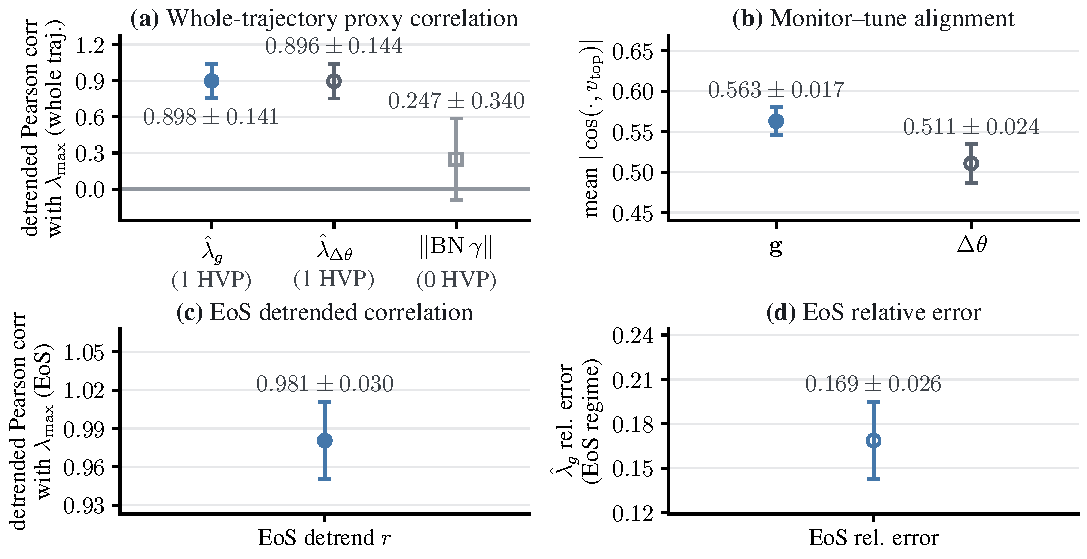
\includegraphics[width=0.9\linewidth]{fig1_rayleigh_monitor_ci.pdf}
\caption{论文图 1（$n=5$ 种子）：$\lhatg$ 是稳健的 $\lmax$ 监测器；Tier-0 的 $\gamma$ 代理种子不稳定（CI 跨零）；原始梯度 $\mathbf{g}$ 与 $\vtope$ 的对齐优于动量更新 $\Delta\theta$。}
\label{fig:ch04-rayleigh}
\end{figure}

图~\ref{fig:ch04-rayleigh} 把本章三条主张压进一张带 CI 的图里，读图时建议按
误差棒而非按均值读：$\lhatg$ 相关系数的种子间散布窄（$\pm0.030$ 量级），与
BN-$\gamma$ 横跨正负的宽 CI 形成对照；对齐面板里 $\mathbf{g}$ 与 $\Delta\theta$
两组误差棒的\emph{不重叠}，正是上面这组对比能当结论而不仅是趋势的全部统计依据。

\subsection{与教程第 9 节的衔接：从入门代理到完整地图}
\label{sec:ch04-practice}

最后把本章放回教程的延长线上。教程第 9 节的结论是“$\lmax$
太贵，权重范数可以当代理”——一个在 tanh MLP
上完全成立的入门命题。论文这一节把它升级为三件事：\textbf{(a)} 代理不止一种，按
HVP 成本排成阶梯；\textbf{(b)} 每层的可靠性是归一化族与训练阶段的函数（plain
范数、BN-$\gamma$、LN 的 $\|\mathbf{g}\|$ 各管一段，且都不稳）；\textbf{(c)}
甜蜜点是单 HVP 的 $\lhatg$，其偏差结构（瑞利 slack）被显式刻画。

由此可以写出论文隐含的\textbf{实践决策表}：
\begin{itemize}
  \item \textbf{训练中后期、已进入 EoS 对齐区}（$|\cos(\mathbf{g},\vtope)|$
高，可由 $\lhatg/\lmax$ 的稳定性侧面印证）：直接信任 $\lhatg$——$+0.981\pm0.030$
的相关加上可预测的约 $17\%$ 瑞利折减，一次 HVP 换一个近乎精确的监测器。
  \item \textbf{训练早期或归一化主导区}（对齐尚未建立）：$\lhatg$
的下界性质会使它系统性偏低且无对齐先验可校准，此时用 $\|\mathbf{g}\|$
兜底（LN/Transformer 上 $+0.52$，且对所有归一化族都是免费量）。
  \item \textbf{BN 网络}：不要在单 seed 上对 $\|\gamma\|$
下任何结论（$+0.247\pm0.340$ 跨零）；宁可付一次 HVP。
  \item \textbf{任何比较代理的实验}：密集采样，勿在 16
点量级的稀疏序列上比相关（窗口摆动可达 $\pm0.25$）。
\end{itemize}

还应注意本章在全文论证中的位置：它建立的“预测端成功”越扎实，后面控制端的失败就越有分量——\textbf{正因为
$\lhatg$ 能以 $+0.981$ 的精度\emph{读出} $\lmax$，用它去\emph{改写} $\lmax$
的失败才不能归咎于“没测准”}。预测器与执行器的分界线，是在预测器最好的位置上画出来的。

\subsection*{本章要点}
\begin{itemize}
  \item 代理阶梯三层：0 HVP 范数 / $\gamma$ 代理（归一化族依赖：plain
$\to\|\mathbf{W}\|$、BN $\to\gamma$、ViT $\to\|\mathbf{g}\|$）$\to$ 1 HVP 的
$\lhatg$ $\to$ 约 5 HVP 的热启动精确测量；甜蜜点是 $\lhatg$。
  \item Tier-0 的三个裂缝：plain 上 last-hidden 最优（$10/14$）但只到
$0.65$--$0.71$；BN 下范数相关由正转负（$-0.8$）、$\gamma$ 接棒但多种子
$+0.247\pm0.340$ 跨零；LN 上所有零计算代理挤在 $0.44$--$0.52$，且 16
点去趋势相关可因窗口摆动 $\pm0.25$。
  \item $\lhatg$ 在二次型下代数等于 $\lambda_c$（Kalra 等 2026，非本文新颖），是
$\lmax$ 的瑞利下界；ResNet 上全程 $+0.898\pm0.141$、EoS
体制（$|\cos|>0.7$）$+0.981\pm0.030$。
  \item 约 $17\%$ 的相对差距 = 瑞利下界的预期 slack（对齐 $0.85$--$0.9
\Rightarrow \cos^{2}\!\approx\!0.8$），有方向、可校准，不是噪声。
  \item 监测探针用原始梯度而非动量更新：对齐与 EoS 误差的 CI 均不重叠（$0.563$
对 $0.511$；$0.169$ 对 $0.238$），全程相关打平（约 $0.90$）——与 CDAT / Kalra
的更新方向用法形成正交分工。
\end{itemize}

% !TEX encoding = UTF-8
% 第五章（解读）：控制端——预测器不是执行器（C1/C2/C3）
% 对应论文 §5 开场、§5.1（C1/C2 范数帽）、§5.2（C3 秩-1 plant）与 Algorithm 1。
% §5.3 见解读第六章（ch06）；§5.4--§5.6 见解读第七章（ch07）；§5.7 见解读第八章。

\section{控制端：预测器不是执行器（C1/C2/C3）}
\label{sec:ch05}

\begin{keybox}{本章速览}
\begin{itemize}
  \item 论文 §5 按\textbf{失败模式}而非按方法组织控制实验：由 proxy 驱动的帽
        （C1/C2）动不了 $\lmax$；秩-1 plant（C3）两种体制都不下逃逸；
        只有 SAM 的全局动作把均衡点压下去。
  \item C1 权重范数帽（norm cap，把权重范数投影回预算球的干预；plain 网）：约 $750/3000$ 步触发，
        $\lmax^{\mathrm{final}}=40.26\pm0.43=2/\eta$，无逃逸。
  \item C2 $\gamma$-帽（BN 网）：$\lmax^{\mathrm{final}}=81.6\pm19.2$
        vs 基线 $73.0\pm12.9$，无逃逸，精度还略差（$0.754$ vs $0.768$）。
  \item C3 秩-1 阻尼：滞后 $\hat v$ 钉在 $2/\eta$（体制 (i)，
        $40.12\pm0.12$）；精确 $\hat v$ 上逃逸到 $261.8\pm5.4$
        （体制 (ii)）——两个结局都背向控制目标。
  \item 只有 SAM 全局扰动下行：$21.35\pm0.04<40$。
\end{itemize}
\end{keybox}

\paragraph{本章在论文中的位置。}
论文的核心论点``sharpness proxy 是预测器、不是执行器''，其前半（预测端）已在
论文第 2--4 节站稳了脚跟；从 §5 开始转向控制端，问的是反过来的
问题：能否用这些便宜的 proxy（或它们指向的曲率信息）\emph{驱动}训练离开 EoS
均衡点（``点''是行文习惯——均衡实指那条 $\lmax\approx2/\eta$ 的
周期-2 振荡轨道，见第九章）？本章覆盖论文 §5 的开场、§5.1（C1/C2 两个范数帽控制）与 §5.2（C3
秩-1 plant——论文自称``最干净的实验''），并转述 Algorithm 1 的逻辑。§5.3
（SAM 逃逸与 X-SAM 消融）在解读第 \ref{sec:ch06} 章；§5.4--§5.6 的三个压力
测试（谱迁移反驳、正交阻尼与传感滞后、clamp-free 桥）在第 \ref{sec:ch07}
章；第四个压力测试——ResNet-18/CIFAR-100 规模复现（§5.7）——留给解读第八章。

\subsection{组织逻辑：按失败模式排列的控制实验}
\label{sec:ch05-organization}

回忆引言里把``用 sharpness proxy 造优化器''拆成的两问：\textbf{预测/监控}
（proxy 是否跟踪 $\lmax$——是）与\textbf{控制/驱动}（proxy 能否把训练推离
$2/\eta$ 均衡——否）。§5 的实验排布不是按``试了哪些方法''罗列，而是按
\emph{失败模式}分成三类，每一类排除一种候选执行器：

\begin{enumerate}
  \item \textbf{由 proxy 驱动的帽（C1、C2，§5.1）}：把 proxy 本身（plain 网
        的权重范数、BN 网的 $\gamma$）投影住，看 $\lmax$ 是否跟着走。
        结果：不动。
  \item \textbf{秩-1 plant（C3，§5.2）}：不再约束 proxy，而是直接改写梯度
        ——与 SAM 同类的 plant 干预（直接改写梯度的执行器干预）。结局由
        特征向量估计 $\hat v$ 的精度决定，两种体制都不下逃逸：不完美阻尼
        留下自稳定帽（钉在 $2/\eta$，体制 (i)）；精确阻尼移除帽
        （上逃逸，体制 (ii)）。
  \item \textbf{全局动作（SAM，§5.3）}：唯一把均衡点压到阈值以下的。
\end{enumerate}

这个排序要成立，必须扛过四个压力测试，分别堵住四种替代解释：
``锐度其实搬到了未阻尼的方向''（谱迁移，§5.4$\to$\ref{sec:ch07}）；
``你阻尼错了方向/传感器太旧''（正交阻尼与滞后，§5.5$\to$\ref{sec:ch07}）；
``执行器根本没开火，是钳位休眠''（clamp-free 桥，§5.6$\to$\ref{sec:ch07}）；
``小 MLP 怪癖''（规模复现，§5.7$\to$解读第八章）。

术语提醒（与论文术语表一致）：\textbf{下逃逸}（flat-escape）$=$ 把 $\lmax$
严格压到阈值以下——声明的控制目标；\textbf{上逃逸}（sharp-escape）$=$ 帽被
移除后冲过阈值向上；\textbf{自稳定帽} $=$ $2/\eta$ 这个由周期-2 EoS 振荡
维持的自稳定上限；\textbf{有动作仍被钉住}（pinned despite action）$=$ 执行
器全力开火（实测、非休眠）而 $\lmax$ 仍留在跨种子噪声包络内——这是规模实验
（§5.7）的现象，第八章展开。

\subsection{C1/C2：帽住 proxy 本身，$\lmax$ 不跟}
\label{sec:ch05-normcaps}

设计动机直白：论文前半篇证明了这些零计算量的 proxy 在监控意义上可用
（plain 网 $\to\|\mathbf{W}\|$、BN 网 $\to\gamma$）。最自然的``控制化''就是
把 proxy 本身帽住——如果 proxy 与 $\lmax$ 的耦合是双向的，帽住 proxy 应该
连带把 $\lmax$ 拉下来。两个控制分别在两种归一化家族里做。

\paragraph{C1（plain 网）：权重范数帽。}
对最后隐层权重 $\mathbf{W}_{\mathrm{lh}}$（教程与论文预测端中最好的单层
proxy）做投影：当 $\|\mathbf{W}_{\mathrm{lh}}\|$ 超出预算
$1.01\cdot\|\mathbf{W}_{\mathrm{lh}}\|_{\mathrm{init}}$ 时投影回球面。投影
不是摆设：约 $750/3000$ 步触发（逐 seed
$745/751/746/745/723$，$n{=}5$）——大约每四步就有一次实际动作。结局：
\[
  \lmax^{\mathrm{final}}=40.26\pm0.43=2/\eta ,
\]
无逃逸；峰值在种子噪声内没有降低。这是``有动作仍被钉住''的全批版本：执行
器在持续触发，$\lmax$ 对此没有响应。

\paragraph{C2（BN 网）：$\gamma$-帽。}
在 BatchNorm 网络上 $\|\mathbf{W}\|$ 失效（相关性翻负），正确的 proxy 家族
是 BN-$\gamma$（$\gamma$ 即 BN 层的逐通道仿射缩放参数，$\|\gamma\|$
为何能接棒权重范数的机制见第~\ref{sec:ch04}~章）。C2 把所有 BN-$\gamma$ 投影到
$1.02\cdot\|\gamma_{\mathrm{init}}\|$。结局：
$\lmax^{\mathrm{final}}=81.6\pm19.2$ vs 基线 $73.0\pm12.9$——点估计
不降反升、两臂 CI 重叠且干预臂更宽（按第~\ref{sec:ch03-stats}~节的
判读规则：检测不到任何下降，方向性证据也不支持下降），精度还略差
（$0.754$ vs $0.768$）。

\paragraph{两点教训。}
其一，换到``正确的 proxy 家族''也一样失败——失败不在选错 proxy，而在
\emph{proxy 造不出执行器}这一结构本身：帽住的是一个与 $\lmax$ 相关的量，
不是 $\lmax$ 的因果杠杆；权重范数被钉住的同时，网络仍把曲率维持到 $2/\eta$。
相关性撑得起预测器，撑不起执行器——这是``predictor $\ne$ actuator''最直接
的实验形式。其二，控制不是免费的：C1 每四步触发一次、C2 付了精度，都没有
换来 $\lmax$ 的移动。

\subsection{C3：秩-1 plant——最干净的实验}
\label{sec:ch05-rank1}

C1/C2 帽的是 proxy；C3 直接改写梯度——与 SAM 同类的 plant 干预（plant
是控制论里“受控对象/装置”的行话，本文转指“直接伸手改写梯度”的
干预，见第~\ref{sec:ch00-glossary}~节背景速查）。设计：取
top 特征向量估计 $\hat v$（单位长度），把梯度按 $\hat v$ 分解并阻尼平行
分量（之所以叫“秩-1”：梯度改写算子只含
$\hat v\hat v^{\!\top}$ 这一个方向的外积、矩阵秩为 1——类比 LoRA 的
低秩更新，但作用在梯度上且是削减；rank-$k$ 即同时缩放前 $k$ 个特征
方向、秩为 $k$）：
\begin{equation}
  \Delta\theta=-\eta\left(\mathbf{g}_{\perp}+\mathbf{g}_{\parallel}/d\right),
  \qquad
  d=\max\!\left(\hat\lambda/(2/\eta),\,1\right),
  \qquad
  \hat\lambda=\hat v^{\!\top}\!H\hat v,
  \label{eq:ch05-rank1}
\end{equation}
其中 $\alpha=\langle\mathbf{g},\hat v\rangle$、
$\mathbf{g}_{\parallel}=\alpha\hat v$、
$\mathbf{g}_{\perp}=\mathbf{g}-\alpha\hat v$；$\hat\lambda$ 只需一次
Hessian--向量积（HVP）。钳位门控 $d=\max(\cdot,1)$ 是自门控（clamp，
截断）：“门控”指只在条件满足时才放行干预——此处即只在感知到的锐度
超过目标 $2/\eta$ 时阻尼、低于目标时更新退化为原始 SGD；“自”指开门
条件由自己测得的量（$\hat\lambda$）决定。

\paragraph{Algorithm 1 的文字转述。}
论文的 Algorithm 1 给出 C3 与 clamp-free 桥变体的统一流程，逻辑如下：
\begin{itemize}
  \item \textbf{输入}：步长 $\eta$、梯度 $\mathbf{g}=\nabla L(\theta)$、
        单位向量 $\hat v$（来源三选一：free-lagged（零成本但滞后一步：
        直接拿上一步的更新方向当这一步的估计）、幂迭代或 ARPACK 传感）、
        目标 $\lambda_{\mathrm{targ}}=2/\eta$、变体标记
        $\in\{\text{clamped},\text{clamp-free}\}$。
  \item \textbf{分解}：$\alpha\gets\langle\mathbf{g},\hat v\rangle$，
        $\mathbf{g}_{\perp}\gets\mathbf{g}-\alpha\hat v$（把 $\mathbf{g}$
        按 $\hat v$ 切开）。
  \item \textbf{传感}：一次 HVP 得 $\hat\lambda\gets\hat v^{\!\top}H\hat v$。
  \item \textbf{定除数}：$d\gets\hat\lambda/\lambda_{\mathrm{targ}}$。
  \item \textbf{clamped 分支}（默认 C3）：$d\gets\max(d,\,1)$——只在超过
        目标时开火；编辑后梯度
        $\tilde{\mathbf{g}}\gets\mathbf{g}_{\perp}+\alpha\hat v/d$。
  \item \textbf{clamp-free 分支}：$f\gets\mathrm{clip}(1-1/d,\,-1,\,1)$
        ——阈值以下做\emph{有界的}符号翻转反向增强；编辑后梯度
        $\tilde{\mathbf{g}}\gets\mathbf{g}_{\perp}+(1-f)\,\alpha\hat v$
        （语义精读见第 \ref{sec:ch07} 章）。
  \item \textbf{步进}：$\theta\gets\theta-\eta\,\tilde{\mathbf{g}}$。
\end{itemize}
直觉：EoS 上 $\lmax\approx2/\eta$，理想传感下 $d\gtrsim1$，沿 top 方向的
有效步长被压回稳定边界——这是``用锐度信息操纵训练''的最小实现。但结局完全
取决于 $\hat v$ 的精度，而且\emph{两种结局都不是控制目标}。

\paragraph{体制 (i)：free-lagged $\hat v$——不完美阻尼，帽保持。}
取 $\hat v=\Delta\theta_{t-1}/\|\cdot\|$。理由是教程里见过的 Damian 等
(2023) 对齐签名（signature，某机制成立时应出现的特征性数值“指纹”）：EoS 处
$|\cos(\Delta\theta,\vtope)|\to0.998$，上一步的更新方向几乎是免费的
top 特征向量估计。结局：
$\lmax^{\mathrm{final}}=40.12\pm0.12=2/\eta$。滞后的 $\hat v$ 不能完全
抵消 $\mathbf{g}_{\parallel}$，周期-2 EoS 振荡得以存续，自稳定帽保持——
钉在均衡点。

\paragraph{诊断陷阱：$\hat\lambda$ 塌缩不是迁移签名。}
此变体的诊断量 $\hat\lambda=\hat v^{\!\top}H\hat v$ 塌缩到 $\sim10^{-4}$，
而真 $\lmax$ 留在 $40$。表面上这像``锐度从被感知的方向迁走了''（迁移签名
——若锐度真在搬家，应观测到的那种特征模式）；正确读法是 \textbf{$\hat v$-跟踪失败}：随着 plant 的活动窗口改变更新方向
，滞后的 $\hat v$ 转出 $u_{1}$，$\hat\lambda$ 读到的是次主导轴（第二大
特征值对应的方向）。研究日志
（发现 23）记载了这次纠错——早期的``迁移''解读正是在这里被推翻的；第
\ref{sec:ch07} 章会在专为此构造的景观上把迁移假说彻底关掉。

\begin{figure}[!ht]
\centering
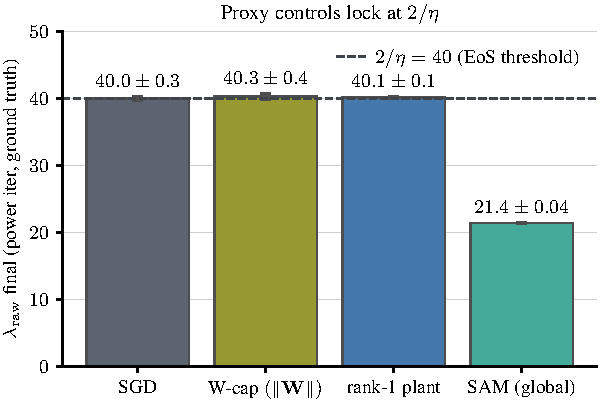
\includegraphics[width=0.62\linewidth]{26_multiseed_control_results.pdf}
\caption{多种子控制结果（论文图 26；误差棒为 $95\%$ CI，所有臂 $n{=}5$）：
W-帽（C1）与 free-lagged 秩-1 plant（体制 (i)）都锁在 $2/\eta$，只有全局
的 SAM 逃逸到下方。（精确 $\vtope$ 的秩-1 变体——体制 (ii)——反而上逃逸到
$2/\eta$ 之上，见图 \ref{fig:ch05-rankk}；$\gamma$-帽控制 C2 见正文。）}
\label{fig:ch05-control}
\end{figure}

\paragraph{体制 (ii)：accurate $\hat v$（精确估计）——精确抵消，帽被移除，上逃逸。}
把 $\hat v$ 换成热启动幂迭代的精确估计（即论文 rank-$k$ sweep（sweep，扫描）的 $k{=}1$
臂）：$\lmax^{\mathrm{final}}=261.8\pm5.4$。机制：抵消现在是精确的
（$\eta_{\mathrm{eff}}\lambda_{1}=2$；$\eta_{\mathrm{eff}}$ 为阻尼后
顶部方向的有效步长），周期-2 振荡被杀死，自稳定帽被移除
，渐进尖锐化无遮拦地把 $\lmax$ 推过 $2/\eta$——\textbf{上逃逸}，与控制
目标正好相反。

附带一个反直觉结果：上逃逸臂的 train loss 更低（$0.090$ vs $0.111$），
held-out 测试 MSE 也更低（$0.0932$ vs $0.1142$，$n{=}5$）——但最小值
\emph{更尖、不平坦}。锐度本身并没有换来泛化惩罚；论文讨论节的 Limitations
(vi) 对这一单任务反例做了 scope 限定。

\begin{figure}[!ht]
\centering
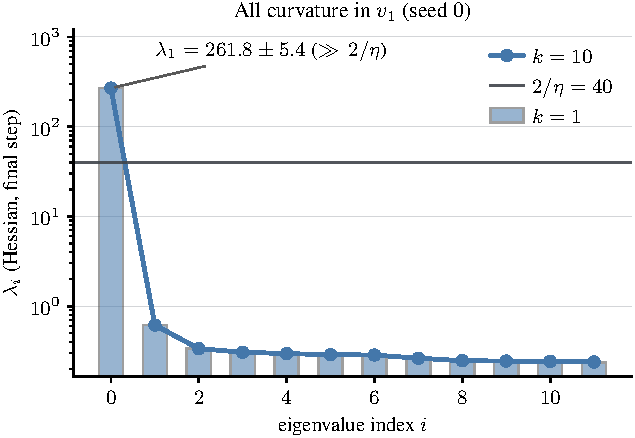
\includegraphics[width=0.62\linewidth]{27_rankk_sweep.pdf}
\caption{rank-$k$ sweep（sweep，扫描；论文图 27）：1-D sharp（一维
尖锐：谱里只有 $\lambda_1$ 一个尖方向）的 teacher--student 景观在
精确幂迭代 $\vtope$ 阻尼后的 top-12 海森谱（seed 0，$n{=}5$）。谱是
1-D sharp：$\lambda_{1}=261.8\pm5.4\gg2/\eta$ 而
$\lambda_{2}\approx0.6$——除 top 外无处可迁；$k{=}1,2,5,10$ 逐 bit 相同
，正是``帽移除''的预言（``迁移''则预言更多阻尼 $\Rightarrow$ 更低
$\lmax$，与观测相反）。}
\label{fig:ch05-rankk}
\end{figure}

图 \ref{fig:ch05-rankk} 同时为第 \ref{sec:ch07} 章埋下伏笔：迁移读法需要
第二个尖方向才有地方搬，而默认景观是 1-D sharp
（$\lambda_{1}=261.8\pm5.4\gg\lambda_{2}\approx0.6$）——所以论文干脆构造
一个两方向同钉 $2/\eta$ 的景观，在迁移唯一可能起作用的地方检验它。

\paragraph{``re-acquire $\vtope$''（重新获取/刷新特征向量）变体为何锁死在 $2/\eta$。}
该变体最终锁定 $40.019\pm0.002=2/\eta$，曾被读作``即使刷新特征向量也不逃
''的独立证据。真相是实现冗余：每步末刷新的 $\vtope$ 会在下一步被 free
$\Delta\theta$ 覆写（$\hat v\leftarrow\mathrm{unit}(\Delta\theta)$），于是
它除刷新后的单步外全程退化为 free-lagged 变体——体制 (i)，不是独立结局。
真正``每步精确 $\vtope$''的测试是带持久热启动的 rank-$k$ sweep（上一段）
，它落在体制 (ii)。研究日志（发现 23）把这次纠错列为必须主动承认的方法论
缺陷——论文以此为例展示了如何把一个看似支持自己的假证据识别并撤回。

\subsection{与教程的衔接：给自稳定振荡装上执行器的两种结局}
\label{sec:ch05-tutorial}

教程第 7 节展示了周期-2 振荡与自稳定化：$\lmax$ 爬到 $2/\eta$，Damian
三阶项把振荡振幅稳住，形成自稳定帽。本章做的事是\emph{用执行器干预它}，
并展示仅有的两种结局：阻尼不完美（体制 (i)）$\to$ 振荡留存 $\to$ 帽留存
$\to$ 钉在 $2/\eta$；阻尼精确（体制 (ii)）$\to$ 振荡被杀死 $\to$ 帽被移除
$\to$ 上逃逸过 $2/\eta$。唯独没有的结局是``压到 $2/\eta$ 以下''——单方向
阻尼做不到；只有 SAM 的全局扰动
（$\varepsilon=\rho\,\mathbf{g}/\|\mathbf{g}\|$，Foret 等 2021；SAM 的
两步算法与``全局''的数学含义见第~\ref{sec:ch01}~章的概念详解框）把均衡点
带到 $21.35\pm0.04<40$。为什么全局动作能而局部动作不能、这个排序如何扛过
四个压力测试，是第 \ref{sec:ch06}、\ref{sec:ch07} 章与解读第八章的主题。

\subsection*{本章要点}
\begin{itemize}
  \item \textbf{C1/C2：帽住 proxy 不动 $\lmax$。}权重范数帽频繁触发
        （$\sim750/3000$ 步）仍锁 $2/\eta$（$40.26\pm0.43$）；BN-$\gamma$
        帽不降反宽（$81.6\pm19.2$ vs $73.0\pm12.9$）且精度略差（$0.754$
        vs $0.768$）——相关性可作预测器、不可作执行器。
  \item \textbf{C3 体制 (i)：}free-lagged $\hat v$ 阻尼不完美，周期-2
        振荡与自稳定帽留存，$\lmax$ 钉在 $2/\eta$（$40.12\pm0.12$）；
        $\hat\lambda$ 塌缩到 $\sim10^{-4}$ 是 $\hat v$-跟踪失败，不是
        迁移签名。
  \item \textbf{C3 体制 (ii)：}精确 $\hat v$ 使
        $\eta_{\mathrm{eff}}\lambda_{1}=2$，振荡被杀死、帽被移除，上逃逸
        到 $261.8\pm5.4$——与控制目标相反；逃逸臂的 loss 与测试 MSE 反而
        更低（$0.090$/$0.0932$ vs $0.111$/$0.1142$），但最小值更尖。
  \item \textbf{``re-acquire'' 变体的 $40.019\pm0.002$}是覆写造成的退化
        （体制 (i)），不是独立证据——一个被主动撤回的假支持证据。
  \item \textbf{排序成立：}proxy 帽与单方向 plant 都不下逃逸，只有 SAM
        全局动作下行——该排序将经受四个压力测试
        （第 \ref{sec:ch07} 章与解读第八章）。
\end{itemize}

% !TEX encoding = UTF-8
% 第六章（解读）：X-SAM 消融——逃逸属于全局分量
% 对应论文 §5.3（Only SAM escapes; the X-SAM ablation）与图 28。

\section{X-SAM 消融：逃逸属于全局分量}
\label{sec:ch06}

\begin{keybox}{本章速览}
\begin{itemize}
  \item 问题：X-SAM（Duan 等，2026）在 SAM 上叠加秩-1 顶部特征向量修正，
        声称``显式约束 $\lmax$''；论文检验该修正是否有可检测的贡献。
  \item 四臂对比：CIFAR-10/ResNet-18、确定性 CUDA、$n{=}10$——
        SGD / SAM($\rho{=}0.05$) / faithful X-SAM（Duan Eq.~11：
        固定 $\alpha{=}0.2$、无钳位、符号门控、每步触发）/ clamped 变体
        （$d=\max(\hat\lambda/(2/\eta),1)$）。
  \item 晚期（步 $\geq3000$）真 $\lmax$：SGD $31.1\pm2.3$、SAM
        $23.3\pm1.6$、faithful $23.9\pm1.6$、clamped $23.4\pm1.6$
        ——三个 SAM 族 CI 重叠。
  \item 配对差（paired difference，同种子配对相减再统计：两臂共享同一
        种子的难度与数据噪声，相减后这些共同波动被约掉、只剩优化器本身
        的差异——同样的种子数能分辨更小的效应）$\Delta\lmax(\text{faithful}-\text{SAM})=+0.62\pm1.23$
        （晚期）、$+0.59\pm2.55$（中期），CI 均跨零；晚期效应量上界
        $+1.85$（效应量 = 真实差异的大小；上界即其 CI 上端——真实差异
        再大也大不过它），小于 SAM 晚期绝对 $\lmax$ 的 $\sim8\%$。
  \item 测量纪律：ARPACK 真 $\lmax$（确定性 512 样本批、$k{=}3$、
        $\mathrm{tol}{=}10^{-6}$）；小批幂迭代在该交叉熵海森上伪收敛
        （平均低估 $+45\%$，实测）。
\end{itemize}
\end{keybox}

\paragraph{本章在论文中的位置。}
本章对应论文 §5.3。第 \ref{sec:ch05} 章建立的机制排序——proxy 帽与单方向
plant 都不下逃逸、只有 SAM 全局动作下行——在这里变成对第三方方法的
\emph{可证伪检验}：如果排序正确，那么任何``SAM $+$ 单方向修正''的组合，其
逃逸都应来自 SAM 分量，修正本身不应有可检测的贡献。X-SAM（Duan 等，2026）
正是这样一个组合，且作者声称其修正``显式约束 $\lmax$''——这是一个直接
冲突，必须实测。本章的副产品——钳位门控可以制造休眠——直接催生第
\ref{sec:ch07} 章的 clamp-free 桥；本章确立的确定性噪声地板标准，后来也用来
重验规模实验的三向排序（解读第八章）。

\subsection{问题设定：把机制排序变成可证伪检验}
\label{sec:ch06-question}

X-SAM $=$ SAM 的全局扰动
（$\varepsilon=\rho\,\mathbf{g}/\|\mathbf{g}\|$，Foret 等 2021）
$+$ 沿 top 特征向量的秩-1 梯度修正——结构上正是``全局动作 $+$ 第
\ref{sec:ch05} 章的秩-1 plant''。Duan 等 (2026) 的框架是``显式约束
$\lmax$''。论文的机制猜想（第 \ref{sec:ch05} 章 C3 的两体制结论）预言：
骑在 SAM 上的秩-1 修正不应有超越 SAM 的可检测贡献；孤立的秩-1 修正（无
SAM 底座）在 MLP 测试床上不仅起不到约束作用，反而会按体制 (ii) 上逃逸。如果
faithful X-SAM 显著低于 SAM，机制排序就要修正——所以这是一个真正可证伪
的检验，而不是走过场的消融。

\subsection{四臂设计与测量纪律}
\label{sec:ch06-design}

\paragraph{四臂。}CIFAR-10/ResNet-18，\emph{确定性} CUDA 模式，$n{=}10$
种子：
\begin{itemize}
  \item \textbf{SGD}：基线；
  \item \textbf{SAM}（$\rho{=}0.05$）：全局扰动底座；
  \item \textbf{faithful X-SAM}：忠实实现 Duan 等 Eq.~11——固定
        $\alpha{=}0.2$（此 $\alpha$ 为 Duan 算法的固定修正幅度超参，
        与第五章的梯度分量 $\alpha=\langle\mathbf{g},\hat v\rangle$
        无关）、无钳位、符号门控（sign-gated，只取内积
        $\langle g,v\rangle$ 的正负号、不管其大小，来决定修正的方向）、无条件每步触发；
  \item \textbf{clamped 变体}：$d=\max(\hat\lambda/(2/\eta),1)$——即论文
        自家 C3 门控的保守消融臂。
\end{itemize}

\paragraph{测量纪律一：CUDA 非确定性。}
默认的 conv 反向传播是非确定的：两个完全相同的 SAM run 会发散到
$\sim10^{-1}$ 的终态参数差，产生 $\sim6$ 单位的伪 $\lmax$ 差距——若不
加控制，跨优化器的单种子 $\lmax$ 比较会被 CUDA 噪声主导。确定性模式消除
之。这是本章的第一条方法论教训：\emph{在比较 $\lmax$ 之前先证明两个相同
 run 逐位重合}。

\paragraph{测量纪律二：估计器伪收敛。}
小批幂迭代估计在该交叉熵海森上\emph{伪收敛}（false convergence）——平均
低估 $+45\%$（直接实测的数字）。因此论文报告 ARPACK 真 $\lmax$：确定性
512 样本批、$k{=}3$、$\mathrm{tol}{=}10^{-6}$。这与论文预测端的主题呼应：
便宜的锐度估计器有明确的失效区，用它测量之前必须先诊断——同一教训在规模
实验（解读第八章）里还会以更大的代价重演一次。

\subsection{结果：null——三个 SAM 族臂不可区分}
\label{sec:ch06-result}

\paragraph{真 $\lmax$。}
晚期（步 $\geq3000$）、$n{=}10$、mean$\pm95\%$ CI：
\begin{center}
\begin{tabular}{lc}
\toprule
优化器 & 晚期真 $\lmax$ \\
\midrule
SGD & $31.1\pm2.3$ \\
SAM & $23.3\pm1.6$ \\
faithful X-SAM & $23.9\pm1.6$ \\
clamped X-SAM & $23.4\pm1.6$ \\
\bottomrule
\end{tabular}
\end{center}
三个 SAM 族臂的 CI 重叠。配对差
$\Delta\lmax(\text{faithful}-\text{SAM})$ 为 $+0.62\pm1.23$（晚期）、
$+0.59\pm2.55$（中期）——两个 CI 都跨零。晚期效应量上界 $+1.85$（CI
上界）：\emph{在该功效（statistical power，检出给定大小效应的能力：
种子越少、噪声越大，功效越低、只能检出大效应——故``检测不到''不等于``效应为零''；本设计 $n{=}10$、配对差半宽 $\pm1.23$，等价于把大于
$+1.85$ 的效应排除在 95\% 置信之外——这就是``该功效''的定量内容）下，任何低于 SAM 的秩-1 降压都小于 SAM 晚期绝对
$\lmax$ 的 $\sim8\%$（$1.85/23.3\approx7.9\%$；区间 $[-0.61,+1.85]$
同时界住了\emph{有利}方向：任何降压效应至多 $0.61\approx$ SAM 水平
的 $2.6\%$）。}

\paragraph{精度。}
$n{=}10$ 终精度：SGD $0.802$、SAM $0.817$、faithful $0.814$、clamped
$0.815$（都在 $\pm0.02$ CI 内）。faithful X-SAM 不在 SAM 之上——反而低
$0.3$ 点。锐度上检测不到的贡献，也没有带来任何精度增益。

\paragraph{两个补充事实钉死``逃逸属于全局分量''。}
其一，SAM 在该 CIFAR-10 设置下比 SGD 低 $\sim8$ 单位（CIFAR-100 三向差
$\sim7$，见解读第八章），无论秩-1 修正是否骑在上面。其二，孤立的 rank-1
（无 SAM 底座）在第 \ref{sec:ch05} 章的 MLP 测试床上不是约束器而是帽移除
器——上逃逸到 $261.8\pm5.4$（体制 (ii)）。合起来：单独使用时它把帽向上
移除；骑在 SAM 上时贡献低于确定性噪声地板（论文用语，未单独给出数值
——定性指确定性协议下剩余的种子噪声尺度；与之相对，第~\ref{sec:ch03-determinism}~节的
非确定性 CUDA 伪差距约 $6$ 单位，配对差半宽为 $\pm1.23$）。逃逸\emph{压倒性地}是全局 SAM
分量。

\begin{figure}[!ht]
\centering
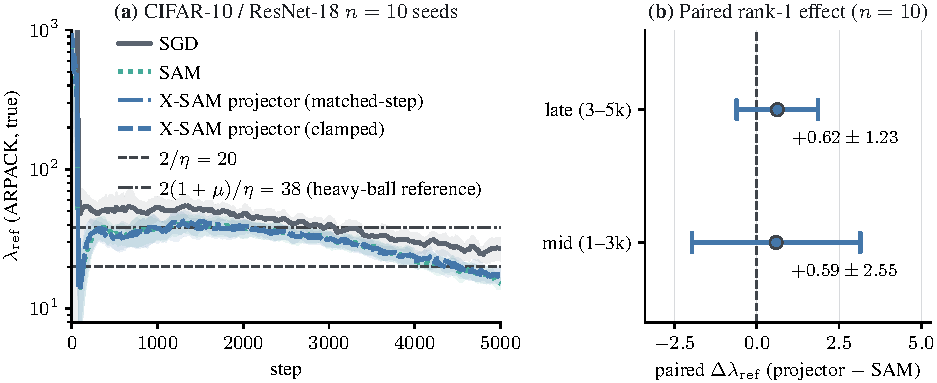
\includegraphics[width=0.95\linewidth]{28_xsam_ablation.pdf}
\caption{X-SAM 消融（论文图 28）：CIFAR-10/ResNet-18，$n{=}10$ 确定性种子，
ARPACK 真 $\lmax$。(a) $\lmax$ 轨迹（粗线为种子均值、阴影为 $95\%$ CI）：
SAM、faithful X-SAM、clamped X-SAM 都降到 SGD 之下，且
faithful$\approx$clamped$\approx$SAM。(b) 配对差
$\Delta\lmax(\text{faithful}-\text{SAM})$（中期与晚期）：CI 均跨零
（晚期 $+0.62\pm1.23$、上界 $+1.85$）——该功效下检测不到秩-1 修正对
$\lmax$ 的效应。孤立 rank-1 消融（无 SAM 底座；MLP 测试床）上逃逸到
$\lmax=261.8\pm5.4$（正文）。}
\label{fig:ch06-xsam}
\end{figure}

\subsection{对 Duan 协议的三点偏离（忠实性声明）}
\label{sec:ch06-fidelity}

论文明确：这是受控的 $\lmax$-\emph{动力学}比较，不是对方精度基准的复现。
Duan 等 (2026) 的设置：CIFAR-10/ResNet-18、SGD 底座、cosine lr $0.1$、
weight decay $5{\times}10^{-5}$、批 $256$、$200$ epochs、flip/pad/crop
增强、$\rho{=}0.05$、$\alpha{=}0.2$、$3$ runs；他们在该设置下报告 X-SAM
$94.71\pm0.20$ vs SAM $93.64\pm0.30$，以及跨 CIFAR-10 骨干 $+1.21\%$
平均 / $+2.08\%$ 最大。三点偏离：

\begin{enumerate}
  \item \textbf{梯度归一化}：他们的 Alg.~2 沿\emph{单位化的}修正梯度更新
        ——步长与损失尺度解耦，修正效应与每步学习率的变化混淆。本文的
        faithful 臂把符号门控投影
        $P_t=I-\alpha\,\mathrm{sign}(\langle g,v\rangle)\,vv^{\top}$
        （即其 Eq.~11 修正）施加于\emph{原始}对抗梯度，使有效步长 $\eta$
        在 SGD/SAM/X-SAM 之间匹配——否则比较的不是修正本身，而是一次隐蔽
        的调 lr。
  \item \textbf{日程}：$5000$ 步（$\approx13$ epochs）、恒定 lr $0.1$、
        批 $128$、weight decay $5{\times}10^{-4}$、无增强、确定性 CUDA
        ——为 $n{=}10$ 的种子级可复现而选，而非峰值精度；对方的精度数字
        出自 200 epoch 增强食谱，与本设置不可直接对比。
  \item \textbf{特征向量刷新}：热启动幂迭代、每步 5 次 HVP、HVP 期间冻结
        BN 统计——比对方的间歇估计更新鲜；若修正有效应，这里的版本只会
        \emph{更强}。
\end{enumerate}

\subsection{null 结果的含义与边界}
\label{sec:ch06-interpretation}

\paragraph{含义。}
在 matched-$\eta$ 动力学（matched-$\eta$ dynamics，各臂有效步长被对齐后的公平动力学比较）下，秩-1 修正对 $\lmax$ 与精度的贡献都检测不到
（晚期上界 $+1.85$，$<8\%$）；``显式约束 $\lmax$''的表述不被支持。第
\ref{sec:ch05} 章的机制排序由此从猜想升级为实测：逃逸属于全局分量。

\paragraph{边界（诚实清单）。}
其一，这个界只覆盖 matched-$\eta$ 动力学——对方 Alg.~2 的归一化更新未测
；其二，全协议复现（cosine 日程、增强、归一化更新、200 epochs）仍是
gap；其三，null 是``在此功效下检测不到''，不是``效应为零''——效应量上界
$+1.85$ 就是这句话的定量形式。

\paragraph{副产品 $\to$ 第 \ref{sec:ch07} 章。}
消融暴露了一个尴尬的自家问题：clamped 臂的秩-1 修正 $0\%$ 步触发，而
faithful $100\%$——$\max(\cdot,1)$ 钳位可以\emph{制造休眠}（dormant）。
而论文的 at-scale 秩-1 plant 用的是同一个钳位，其``惰性''判定——触发比例（fired fraction，执行器实际发挥作用的步数占比）
$\le4\%$、$\approx$SGD——部分是基于这个观察作出的——它也因此沾上了同样
的嫌疑：也许真正中和它的是钳位、不是景观。这个怀疑必须正面处理，就是第
\ref{sec:ch07} 章的
clamp-free 桥。

\subsection*{本章要点}
\begin{itemize}
  \item \textbf{null 结果}（null result，在给定统计功效下检测不到差异的阴性结果）：晚期真 $\lmax$ 三个 SAM 族臂 CI 重叠
        （$23.3\pm1.6$ / $23.9\pm1.6$ / $23.4\pm1.6$）；配对差
        $+0.62\pm1.23$（晚期）、$+0.59\pm2.55$（中期）均跨零；效应量上界
        $+1.85<\text{SAM 晚期绝对 }\lmax$ 的 $8\%$。
  \item \textbf{精度同样不分}：$0.802$/$0.817$/$0.814$/$0.815$
        （$\pm0.02$ CI 内），faithful 比 SAM 低 $0.3$ 点。
  \item \textbf{逃逸属于全局分量}：SAM 比 SGD 低 $\sim8$ 单位与秩-1
        修正无关；孤立 rank-1 在 MLP 上反而上逃逸到 $261.8\pm5.4$。
  \item \textbf{测量纪律}：CUDA 非确定性可制造 $\sim6$ 单位伪差距（须确定性
        模式）；小批幂迭代在该海森上伪收敛、平均低估 $+45\%$（须 ARPACK）。
  \item \textbf{边界}：界只覆盖 matched-$\eta$ 动力学；全协议复现仍是
        gap；副产品——钳位可制造休眠——催生第 \ref{sec:ch07} 章的
        clamp-free 桥。
\end{itemize}

% !TEX encoding = UTF-8
% 第七章（解读）：机制排除——谱迁移、正交阻尼、滞后、clamp-free 桥
% 对应论文 §5.4（Refuting spectral migration）、§5.5（orthogonal damping
% and sensing lag）、§5.6（clamp-free bridge）；图 29、31、32，表 3。

\section{机制排除：谱迁移、正交阻尼、滞后与 clamp-free 桥}
\label{sec:ch07}

\begin{keybox}{本章速览}
\begin{itemize}
  \item 谱迁移在它唯一可能起作用的景观里也被反驳：两个方向同钉 $2/\eta$
        （$\lambda_{1}=40.1$、$\lambda_{2}=40.0$），只阻尼 $u_{1}$ $\to$
        $u_{1}$ 上逃逸（$40.1\to65.2$，seed 0）而 $\lambda_{2}$ 留在
        $39.6$——无流动；$k{=}1{:}\,64.0<k{=}2{:}\,75.2\approx
        k{=}5{:}\,77.4$——自稳定帽的逐方向结构。
  \item C4 正交阻尼：$d\in\{1,1.5,2,4,8\}$ 全部钉在 $2/\eta\approx40$
        （$0/5$ 发散）；代价是收敛变慢（loss $0.11\to0.59$）、沿 $u_{1}$
        振荡缩小（$|x_{t}|$ $0.18\to0.03$）；$d\geq4$ 时 CI 骤宽
        （$\pm9$ vs $\pm0.3$/$\pm1.7$）——G4（理论缺口之四，见
        第九章）的实测。
  \item 滞后无害、方向不准才致命：滞后但精确的 $\hat u(t-k)$
        （$k{=}1,2,3$）与 $k{=}0$ 数值相同地上逃逸到 $261.8\pm5.4$；滞后
        的更新方向传感器 $\Delta\theta_{t-k}\propto-\mathbf{g}$ 钉在
        $2/\eta$（$40.10\pm0.13$/$40.03\pm0.02$/$40.03\pm0.03$）——
        自致传感失败。
  \item clamp-free 桥：去掉 $\max(\cdot,1)$ 钳位、$100\%$ 触发仍不逃逸
        （$\lhatg=17.14\pm1.21$ vs SGD $18.73\pm1.29$，$\Delta=-1.59$
        在 CI 内；SAM $12.91\pm0.59$，差 $-5.8$）——惰性不是钳位假象。
  \item 研究日志亮点：发现 24 的``0/3000 触发''后来被发现 27 证明是自家
        钳位假象——论文把自家 bug 转化成稳健性检验的实例。
\end{itemize}
\end{keybox}

\paragraph{本章在论文中的位置。}
本章对应论文 §5.4--§5.6，兑现第 \ref{sec:ch05} 章预告的四个压力测试中的
三个（§5.5 一个小节管两个：正交阻尼与传感滞后）。每一个都堵住对秩-1 失败
的一种替代解读：``锐度搬走了''（谱迁移，§\ref{sec:ch07-migration}）；
``阻尼错了方向/传感器太旧''（正交阻尼与滞后，
§\ref{sec:ch07-orth}--\ref{sec:ch07-lag}）；``执行器根本没开火''
（clamp-free 桥，§\ref{sec:ch07-bridge}）。第四个压力测试（规模复现）
在解读第八章。合围之后，``只有全局动作能下行''的排序才算扛住了证伪。

\subsection{谱迁移反驳：在它唯一可能起作用的地方检验}
\label{sec:ch07-migration}

\paragraph{逻辑。}
帽移除说预言：特征向量之间\emph{没有流动}——阻尼 $u_{1}$ 只会让 $u_{1}$
自己失去帽而上逃逸，别的方向不受影响。替代的``谱迁移''
（spectral migration）读法把锐度当作某种守恒预算：阻尼一个方向，锐度应
\emph{搬}到未阻尼的方向。这个读法要成立，前提是存在第二个尖方向可搬。第
\ref{sec:ch05} 章的默认景观是 1-D sharp
（$\lambda_{1}=261.8\pm5.4\gg\lambda_{2}\approx0.6$，图
\ref{fig:ch05-rankk}）——迁移在那里无处着力。所以论文构造了一个迁移
\emph{唯一可能起作用}的景观：多输出各向同性 teacher--student（``各向同性''
即各方向性质相同、无偏好方向——构造出的合成教师在多个方向有对称的
尖锐度，好比人为造出两条等深峡谷，用来测试锐度会不会搬家），其 EoS 谱把
两个方向同时钉在 $2/\eta$：$\lambda_{1}=40.1$、$\lambda_{2}=40.0$。

\paragraph{检验与观测。}
只阻尼 $u_{1}$（秩-1、精确特征向量）。迁移读法的预言：$\lambda_{2}$ 应
升过 $2/\eta$，吸收``守恒的锐度预算''。实际观测（论文图 29）：$u_{1}$
上逃逸（$40.1\to65.2$，seed 0 轨迹示例）而 $\lambda_{2}$ \emph{留在 $39.6$}——
没有流动，且 $\lmax>2/\eta$。迁移被反驳。

\begin{figure}[!ht]
\centering
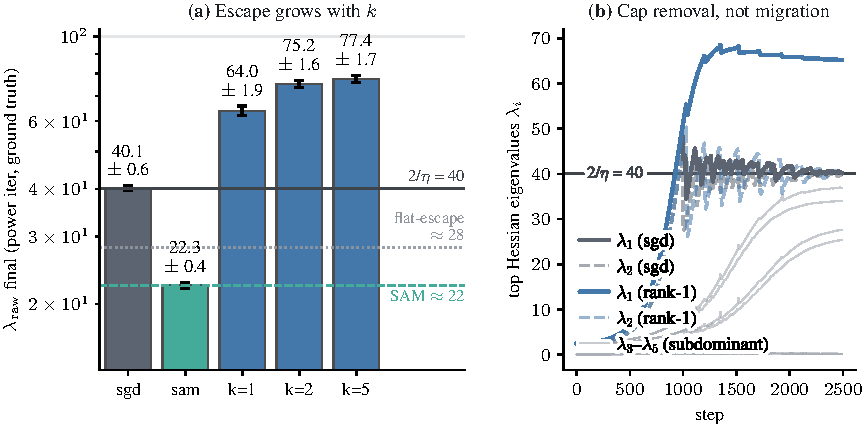
\includegraphics[width=0.95\linewidth]{29_multisharp_migration.pdf}
\caption{多尖锐景观测试（论文图 29；$n{=}5$ 种子）。构造的多输出各向同性
teacher--student 把\emph{两个}方向钉在 $2/\eta$（$\lambda_{1}=40.1$、
$\lambda_{2}=40.0$）。左：只阻尼 $u_{1}$（秩-1）让 $u_{1}$ 上逃逸而
$\lambda_{2}$ 保持钉住——无流动，在迁移貌似可行的地方反驳迁移。右：
$k>1$ 此时起作用，揭示自稳定帽的逐方向结构（数值见正文）。}
\label{fig:ch07-multisharp}
\end{figure}

\paragraph{$k$ 在这里起作用——帽的逐方向结构。}
与 1-D 情形的 $k$-不变（$k{=}1,2,5,10$ 逐 bit 相同）不同，多尖锐景观中
$k$ 有意义：$k{=}1{:}\,64.0<k{=}2{:}\,75.2\approx k{=}5{:}\,77.4$。机制
：每阻尼一个坐在 EoS 帽上的方向 $=$ 移除一个帽 $=$ 该方向独立上逃逸——
$k$ 越大，逃逸的方向越多，$\lmax$ 越高。这反过来确认了帽是\emph{逐方向}（per-direction）
的自治结构：$u_{1}$ 的帽被移除并不连带解除 $u_{2}$ 的帽。顺带一提，多尖锐
景观的上逃逸（$64.0$--$77.4$）远低于 1-D 景观的 $261.8\pm5.4$——每个
方向的曲率质量有限，逃逸有界。

\paragraph{研究日志中的演进。}
日志里这是``option B''：发现 23 在 1-D 景观推翻迁移后，遗留问题是
``$\lambda_{1}\approx\lambda_{2}$ 时迁移是否显形''；发现 25 构造了多尖锐
景观并给出否定答案，论文的理论节（自稳定帽机制）就此定案。数字以论文为
准。

\subsection{C4 正交阻尼：对称控制以对称的方式失败}
\label{sec:ch07-orth}

\paragraph{设计。}
秩-1 plant 阻尼 top 方向；C4（正交阻尼，orthogonal damping，阻尼顶部
方向之外的\emph{全部}正交补——与顶部特征向量垂直的所有参数方向构成
的空间）是对称控制——阻尼\emph{其余一切}：
\begin{equation}
  \Delta\theta=-\eta\left(\mathbf{g}_{\parallel}+\mathbf{g}_{\perp}/d\right),
  \label{eq:ch07-orth}
\end{equation}
保持 top 方向梯度 $\mathbf{g}_{\parallel}$ 原封不动。论文理论节的推论给
出干净预言（$x$-递推指位移变量 $x$ 的迭代式、$y^{*}$ 指均衡时
尖锐度超出阈值 $2/\eta$ 的量——二维状态变量的定义见第九章）：
$\mathbf{g}_{\parallel}$ 保持 $\Rightarrow$ $x$-递推就是无
阻尼的 Damian 映射 $\Rightarrow$ $y^{*}=0$——top 方向的自稳定不受触碰
。

\paragraph{结果：全 $d$ 钉住。}
扫 $d\in\{1,1.5,2,4,8\}$（$n{=}5$，MLP 全批）：$\lmax$ 全部钉在
$2/\eta\approx40$——$40.2,\,40.3,\,38.9,\,43.4,\,40.1$；每个 $d$ 下
$0/5$ 种子发散。

\paragraph{代价与次级现象。}
其一，收敛变慢：最终 loss 从 $0.11$ 升到 $0.59$（$d\to8$）。其二，沿
$u_{1}$ 的振荡缩小：$|x_{t}|$ 从 $0.18$ 降到 $0.03$——补集被冻结后振荡
幅度反而更小，但帽不降。其三，$d\geq4$ 时逐种子散布骤宽：CI $\pm9$
（$d{=}4$）vs $\pm0.3$（$d\leq1.5$）、$\pm1.7$（$d{=}2$）。原因：冻结
补集移走了帮助界定 $u_{1}$ 振荡的方向，常数-$\alpha$ 的 2-D 约简（假设渐进尖锐化系数 $\alpha$ 在窗口内恒定的二维约化，见第九章）失去精度
——这是论文理论 gap \textbf{G4}（缺口之四：二维约化缺少四次及更高阶
景观项、无法给振荡幅度 $|x|$ 定界，见第九章）的实测实例，不是逃逸
（每个 $d$ 下 $0/5$
发散）。

\paragraph{与秩-1 的对照：反向夹逼。}
两个单方向控制以\emph{相反}的机制失败：top 阻尼把帽向上移除（上逃逸过
$2/\eta$，体制 (ii)）；补集阻尼把帽原地留下（钉在 $2/\eta$）。一个向上
、一个不动，都不下逃逸——两个方向一夹，帽的不可下行性得到确认。

\subsection{滞后 vs 方向不准：把混杂变量拆开}
\label{sec:ch07-lag}

\paragraph{混杂。}
第 \ref{sec:ch05} 章体制 (i) 用的延迟更新传感器
$\hat v_{k}=\Delta\theta_{t-k}/\|\cdot\|$ 把两件事混在一起：
\emph{滞后}（信息旧 $k$ 步）与\emph{用错方向}（用更新/梯度方向而非特征
向量）。拆开检验（$n{=}5$，MLP）：

\paragraph{臂 1：滞后但精确——滞后无害。}
传感器 $\hat v_{k}=\hat u(t-k)$（$k{=}1,2,3$；$\hat u$ 为精确的幂迭代
估计，只是旧 $k$ 步）。结果：与 $k{=}0$ \emph{数值相同}地上逃逸到
$261.8\pm5.4$。原因：$u_{1}$ 在慢的 $O(1/\eta)$ 时间尺度上旋转
（即要约 $1/\eta$ 步才明显变化），
$\hat u(t-k)\approx u_{1}(t)$——帽仍被移除。滞后本身无害。

\paragraph{臂 2：滞后且用更新方向——自致传感失败。}
传感器 $\hat v_{k}=\Delta\theta_{t-k}\propto-\mathbf{g}$
（$k{=}1,2,3$）。结果：钉在 $2/\eta$——$40.10\pm0.13$、
$40.03\pm0.02$、$40.03\pm0.03$。起作用的原因不是陈旧而是
\textbf{自致传感失败}（self-induced sensing failure，执行器自己的动作把传感器转离目标方向）：plant 自己的阻尼把更新方向转离 $u_{1}$，执行器随之
脱开。体制 (i) 的根源是\emph{方向不准}，不是滞后。

\paragraph{病理对照：无钳位的执行器病态。}
去掉钳位后，陈旧的瑞利商翻 $\gamma<0$（$\gamma=1-1/d$ 为阻尼强度，
见第九章）、变成反向阻尼（负阻尼——不压制
反而放大振荡）——$k{=}1$ 时在步
$\sim540$ 发散。注意这个发散正是 §\ref{sec:ch07-bridge} clamp-free 语义
精读的对照物：那里的符号翻转被截断、有界；这里的原始因子随陈旧瑞利商
塌缩 $\gamma\to-\infty$、无界。

\begin{figure}[!ht]
\centering
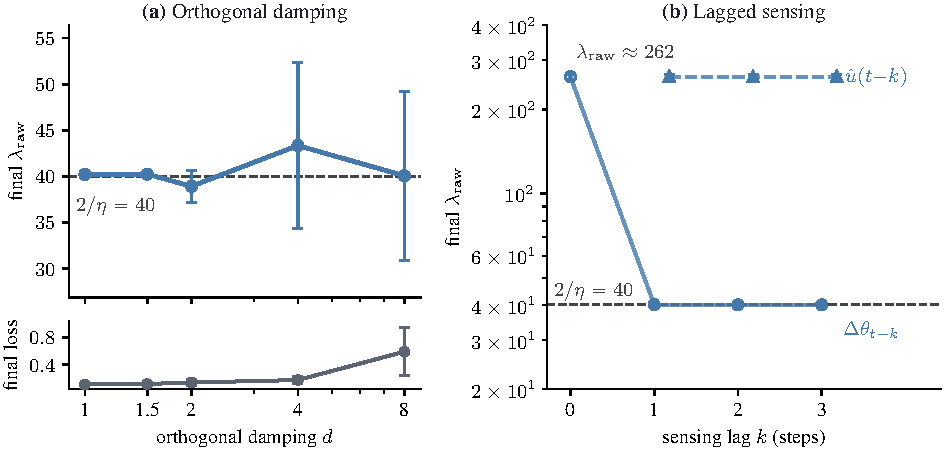
\includegraphics[width=0.95\linewidth]{31_c4_lagged_controls.pdf}
\caption{MLP 全批设置上的两个进一步控制（论文图 31；$n{=}5$ 种子）。
(a) 正交阻尼（C4）：每个 $d\in\{1,\dots,8\}$ 下 $\lmax$ 钉在
$2/\eta\approx40$（$0/5$ 发散；loss 从 $0.11$ 升到 $0.59$，右轴）——
阻尼补集碰不到 top 方向的帽。(b) 滞后 vs 不准：滞后但精确的传感器
$\hat u(t-k)$ 上逃逸到 $261.8\pm5.4$（$\triangle$），与 $k{=}0$ 相同；
滞后的更新方向传感器 $\Delta\theta_{t-k}$ 钉在 $2/\eta$（$\circ$）。
滞后无害；钉住的是梯度方向代理，不是陈旧。}
\label{fig:ch07-c4lag}
\end{figure}

\paragraph{小结。}
帽对传感\emph{滞后}稳健、对传感\emph{不准}不稳健——体制 (i) 的归因由
``旧''改为``偏''。

\subsection{clamp-free 桥：惰性不是钳位假象}
\label{sec:ch07-bridge}

\paragraph{动机：自家门控的嫌疑。}
第 \ref{sec:ch06} 章的 X-SAM 消融给论文自家门控出了一道难题：clamped
X-SAM 的秩-1 修正 $0\%$ 步触发，而 faithful 每步触发——$\max(\cdot,1)$
钳位可以制造休眠（dormant）。而 at-scale 秩-1 plant 用的是\emph{同一个}
钳位，其``惰性''判定（触发比例 $\le4\%$、$\approx$SGD）部分是基于这个
观察作出的——它也因此沾上了同样的嫌疑：也许真正中和它的是钳位、不是景观
。桥接臂正面回：同一 CIFAR-100/ResNet-18 设置、确定性 CUDA、$n{=}5$ 种子、
\texttt{-{}-no-clamp}——无 $\max(\cdot,1)$ 门、每个方向每步都触发
（触发比例 $100\%$）、原始除数 $d=\hat\lambda/\lambda_{\mathrm{targ}}$
允许低于 $1$。

\paragraph{clamp-free 语义精读：不是``总是阻尼''臂。}
编辑（对梯度的手工改写）为 $\mathbf{g}\mapsto\mathbf{g}-f\,\alpha\,\hat v$（其中
$\alpha=\langle\mathbf{g},\hat v\rangle$；$f$ 即编辑因子——对梯度沿
$\hat v$ 分量的改写强度系数），$f=1-1/d$ \emph{截断到}
$[-1,1)$：
\begin{itemize}
  \item $\hat\lambda>\lambda_{\mathrm{targ}}$（$d>1$）：$f\in(0,1)$，
        编辑是阻尼，$\hat v$ 分量留下 $\alpha/d$；
  \item $\hat\lambda<\lambda_{\mathrm{targ}}$（$d<1$）：$f<0$，符号
        翻转——编辑不反对反而\emph{增强} $\hat v$ 分量：有界的反向增强
        （bounded sign-flip anti-damping）；
  \item 截断保证编辑幅度 $\le|\alpha|$、编辑后的 $\hat v$ 分量
        $\le2|\alpha|$——反向增强有界、不会爆炸。
\end{itemize}
与 §\ref{sec:ch07-lag} 的无截断滞后 plant 对比：那里的原始因子随陈旧
瑞利商塌缩 $\gamma\to-\infty$，无界反向阻尼，$k{=}1$ 步 $\sim540$ 发散
；这里符号翻转被截断。\textbf{``是界而不是门''}（门 = 只在条件满足时
才让干预发生；界 = 干预每步都发生、但幅度被截断在固定区间内）把两个
clamp-free 陈述
分开——它们一致而不矛盾。

\paragraph{桥接结果（论文表 3）。}
晚期（步 $\geq2000$）单 HVP 梯度瑞利商 $\lhatg$，确定性 512 样本评估批
，$n{=}5$ 种子，mean$\pm95\%$ CI：

\begin{table}[!ht]
\centering\small
\caption{clamp-free 桥，CIFAR-100/ResNet-18、确定性 CUDA（$n{=}5$ 种子
）：晚期（步 $\geq2000$）$\lhatg$ mean$\pm95\%$ CI 与秩-1 修正的触发比例
（对应论文表 3）。\textbf{仅协议内比较}：$\lhatg$ 是固定评估批上的单 HVP
下界代理，其绝对尺度（13--18）与 at-scale 控制的 ARPACK $\lmax$ 尺度
（22--29）不可比。}
\label{tab:ch07-bridge}
\begin{tabular}{lcc}
\toprule
臂 & 晚期 $\lhatg$ & 触发比例 \\
\midrule
SGD & $18.73\pm1.29$ & --- \\
秩-1（clamped C3） & $18.13\pm1.47$ & $4\%$ \\
\textbf{秩-1（clamp-free C3）} & $\mathbf{17.14\pm1.21}$ & $100\%$ \\
SAM & $12.91\pm0.59$ & --- \\
\bottomrule
\end{tabular}
\end{table}

\paragraph{读数。}
其一，clamp-free 臂\emph{不上逃逸}：与 SGD 差 $\Delta=-1.59$、与
clamped 臂差 $-0.99$——差值量级与两臂 CI 半宽（$1.2$--$1.5$）相当、
区间互相重叠，按第~\ref{sec:ch03-stats}~节的判读规则读作``检测不到
差异''，远不到 MLP 精确
$\vtope$ plant 的上逃逸量级（第 \ref{sec:ch05} 章的 $261.8\pm5.4$）。
其二，clamp-free 比 SGD 低 $\sim1.6$——方向与 Duan 等 (2026) 的预测
一致，但量级远小于 SAM 的 $-5.8$ 且在 CI 内，``贡献可忽略''的裁决不变
。其三，同一驱动重验确定性三向：SAM（$12.91\pm0.59$）低于两个秩-1 臂
且 CI 不重叠——at-scale 排序在 X-SAM 消融引入的更严确定性标准下依然成立。

\paragraph{为何报 $\lhatg$ 而非 ARPACK $\lmax$（within-protocol（协议内——只在同一测量协议之内比较）警告）。}
做桥接实验时，幂迭代 $\lmax$ 估计尚不可信——伪收敛问题后来才在规模实验
（§5.7，解读第八章）中诊断。因此论文报告确定性的 per-model 代理
$\lhatg$（$\lmax$ 的下界代理），所有比较在协议内进行；$\lhatg$ 尺度
（13--18）与 ARPACK $\lmax$ 尺度（22--29）\emph{不可比}——跨协议读数是
本章最容易犯的错误。

\begin{figure}[!htbp]
\centering
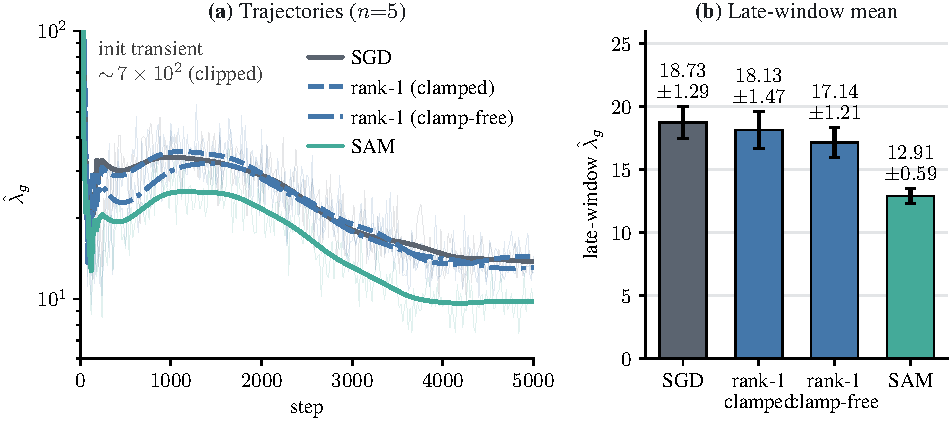
\includegraphics[width=0.92\linewidth]{32_bridge_clampfree_c3.pdf}
\caption{clamp-free 桥（论文图 32；确定性 CUDA，$n{=}5$ 种子）：SGD、
clamped 秩-1、clamp-free 秩-1 与 SAM 的晚期 $\lhatg$
（mean$\pm95\%$ CI；臂用线型与颜色区分，灰度打印下仍可分辨）。
(a) 为对数域高斯平滑后的轨迹（淡细线为未平滑均值，初始瞬态两采样保留未平滑）。
clamp-free 臂每步都触发，却仍在 SGD 与 clamped 臂的 CI 内——无上逃逸、
无钳位假象——而 SAM 以不重叠的 CI 坐在下方。}
\label{fig:ch07-bridge}
\end{figure}

\paragraph{结论：惰性稳健地独立成立。}
对 at-scale 秩-1 结果的两个残余可疑读数——钳位假象与休眠传感器——被
\emph{分别}排除：惰性在去掉钳位（$100\%$ 触发仍不逃逸，
图 \ref{fig:ch07-bridge}）后成立，也在修复传感器（true-$\lmax$ plant：
无钳位地板、ARPACK 传感、全力开火，仍与 sharpness 无关——``有动作仍被
钉住''，详见解读第八章）后成立。

\subsection{研究日志中的演进：一次自我纠错}
\label{sec:ch07-log}

日志里，发现 24（X-SAM 消融第一版）曾断言``rank-1 修正 $0/3000$ 步触发
、结构性死代码''。发现 27 在取得 Duan 等 (2026) 的精确算法（Eq.~11）后
发现：该断言是\emph{自家钳位}（$\max(\cdot,1)$ 自门控）制造的假象——
faithful 版每步触发（$100\%$）。论文吸收了这次纠错：§5.3 改为忠实四臂
对比（第 \ref{sec:ch06} 章），本节的 clamp-free 桥正是把自家的测量伪迹
转化为对 at-scale 判定的稳健性检验。方法论启示：可疑的阴性结果要先排除
``自家仪器造成的休眠''再下结论——而排除的办法，就是把怀疑对象本身变成实验
臂。

\subsection*{本章要点}
\begin{itemize}
  \item \textbf{谱迁移被反驳}：即使在两个方向同钉 $2/\eta$
        （$\lambda_{1}=40.1$、$\lambda_{2}=40.0$）的多尖锐景观，阻尼
        $u_{1}$ 只让 $u_{1}$ 上逃逸（$40.1\to65.2$）、$\lambda_{2}$ 原地
        不动（$39.6$）；$k$ 的作用
        （$k{=}1{:}\,64.0<k{=}2{:}\,75.2\approx k{=}5{:}\,77.4$）揭示帽的
        逐方向结构。
  \item \textbf{C4 正交阻尼}全 $d\in\{1,1.5,2,4,8\}$ 钉在 $2/\eta\approx
        40$（$0/5$ 发散），代价是收敛变慢（loss $0.11\to0.59$）、振荡
        缩小（$|x_{t}|$ $0.18\to0.03$）；$d\geq4$ 时 CI 骤宽（$\pm9$）
        是 G4 的实测——两个单方向控制反向夹逼，都不下逃逸。
  \item \textbf{滞后无害、方向不准致命}：$\hat u(t-k)$ 与 $k{}=0$ 同样
        上逃逸到 $261.8\pm5.4$（$u_{1}$ 在慢 $O(1/\eta)$ 尺度旋转）；
        $\Delta\theta_{t-k}\propto-\mathbf{g}$ 钉在 $2/\eta$
        （$40.10\pm0.13$/$40.03\pm0.02$/$40.03\pm0.03$）——体制 (i) 的
        根源是自致传感失败；无钳位时陈旧瑞利商翻 $\gamma<0$、$k{=}1$ 步
        $\sim540$ 发散。
  \item \textbf{clamp-free 桥}：$100\%$ 触发仍不逃逸
        （$\Delta=-1.59$ vs SGD，在 $\sim1.5$ 单位 CI 内；SAM 的 $-5.8$
        才是真实降幅）；``是界而不是门''把有界反向增强与无截断发散分开
        ；$\lhatg$ 尺度（13--18）与 ARPACK 尺度（22--29）不可比。
  \item \textbf{四个压力测试合围}：单方向控制的失败不是迁移、不是阻尼
        错边、不是传感器太旧、不是钳位休眠——``只有全局动作能下行''的
        排序依然成立；研究日志中``0/3000 触发 $\to$ 自家钳位假象''的纠错
        （发现 24 $\to$ 27）是论文自我纠错的方法论亮点。
\end{itemize}

% ============================================================
% ch08：规模复现：ResNet-18 / CIFAR-100（对应论文 §5.7 "At scale"）
% 读者已读 tutorial/（EoS 入门）；本章讲论文增量。
% ============================================================

\section{规模复现：ResNet-18/CIFAR-100}\label{sec:ch08}

\begin{keybox}{本章速览}
\begin{itemize}
  \item MLP 上的三向对比（SGD / 秩-1 plant / SAM）搬上标准 torchvision
        ResNet-18（11.2M 参数，约为 MLP 的 $160\times$）+ CIFAR-100，$n=5$
        种子、ARPACK + 确定性 CUDA 协议：晚期 $\lmax$ 为 SGD
        $29.21\pm1.90$、rank-1 plant $28.83\pm1.67$、SAM $22.63\pm1.73$。
  \item 诚实读法是\emph{双结局}：SAM 的上置信界（$24.36$）不与
        SGD/rank-1 的下置信界（$27.31/27.16$）重叠，但 SGD 与 rank-1
        之间统计不可分——是 $\{\text{SGD}\approx\text{rank-1}\}$ 与 SAM
        的两方分裂，不是三向分裂。
  \item 一次方法论弯路：原 plant 的幂迭代感知\emph{伪收敛}把真实
        $\lmax\approx36$ 读成 $\approx19$（$+45\%$ 低估），一度被误读为
        “批尖锐度在 $2/\eta$”——\emph{proxy 坏了，不是体制坏了}。
  \item 换上 ARPACK 感知的 true-$\lmax$ plant 后，执行器确以全力开火
        （除数中位 $1.86$、每步阻尼因子 $\approx0.44$），$\lmax$ 仍与
        SGD 重叠：规模版的\emph{有动作仍被钉住}。
  \item 12000 步 + 标准增强的长日程保序（SAM $18.1 <$ SGD $21.9\approx$
        rank-1 $22.8$），且 SAM 精度最好（$0.68$ vs $0.66$）；ResNet-18
        上的 rank-$k$ 是 null 结果，排序结论（任何 $k$ 无下逃逸、唯
        SAM）在真实 CNN 上成立。
\end{itemize}
\end{keybox}

\textbf{本章在论文中的位置。}论文的控制实验（秩-1 阻尼、rank-$k$
扫描、X-SAM 消融、多尖锐景观测试）都发生在全批 GD 的小 MLP 上——这是
EoS 现象最干净的体制，但也是审稿人最容易质疑的地方：\emph{“控制实验都
源自 MLP，结论会不会是 MLP 特异的？”}论文 \S5.7（"At scale"）就是对这个
关切的正面回应：把三向对比（SGD、秩-1 plant、SAM）原样搬到标准
torchvision ResNet-18（11.2M 参数，约为 MLP 的 $160\times$）上，在
CIFAR-100 训练，$n=5$ 种子，并把测量协议升级为确定性 CUDA + ARPACK 直测。
本章按论文顺序讲四件事：三向对比的诚实读法（\S\ref{sec:ch08-threeway}）、
感知伪收敛的方法论插曲与 true-$\lmax$ plant 的“有动作仍被钉住”
（\S\ref{sec:ch08-falseconv}--\S\ref{sec:ch08-pinned}）、更长日程的外部效度
（external validity，结论超出当前实验设置仍然成立的能力；\S\ref{sec:ch08-long}）、以及 rank-$k$ 与“为何 SAM 能而 rank-1
不能”（\S\ref{sec:ch08-rankk}--\S\ref{sec:ch08-why}）。理论一侧的对应
形式化在第~\ref{sec:ch09}~章。

\subsection{先校准阈值：动量下边界是 $2(1+\mu)/\eta=38$，不是 $2/\eta=20$}\label{sec:ch08-threeway}

读者从本解读第 3 章已经知道：$2/\eta$ 定律是\emph{全批 GD} 的极限；在重球
动量（heavy-ball）下，线性稳定性边界移到 $2(1+\mu)/\eta$。ResNet-18 实验
用 $\mu=0.9$（由两边界 $38$ 与 $20$ 可读出 $\eta=0.1$），所以起作用的
边界是 $2(1+\mu)/\eta=38$，而 GD 边界 $2/\eta=20$ 只是参照线。这一步校准
很重要：如果把 20 当作期望钉住值，会误读所有绝对数字。

\textbf{判读口径提醒。}下文``逐种子排序不一致''指同一种子下两臂谁高
谁低在不同种子间来回翻转、无稳定次序——它是``统计不可分''的直观旁证
（判读规则见第~\ref{sec:ch03-stats}~节）。另注意：SGD 与 rank-1 的
判定用的是两臂 CI 重叠加逐种子排序，\emph{未}报告同种子配对差——
配对差能约掉种子间共同波动、分辨力更高（第~\ref{sec:ch06}~章的
X-SAM 消融用的就是它）；若做了配对差，``两臂合并''的读法有可能被
推翻，此处结论以上述较粗的判据为限。

在此校准下，晚期训练（步 $\ge2000$）的 $\lmax$ 均值 $\pm95\%$ 置信区间
（ARPACK、确定性 512 样本评估批、确定性 CUDA、$n=5$ 种子）为：

\begin{table}[!ht]
\centering
\begin{tabular}{lccc}
\toprule
臂 & 晚期 $\lmax$（步 $\ge2000$） & 95\% CI & frac${}<38$ \\
\midrule
SGD & $29.21$ & $\pm1.90$（下界 $27.31$） & $81\%$ \\
rank-1 plant & $28.83$ & $\pm1.67$（下界 $27.16$） & $82\%$ \\
SAM & $22.63$ & $\pm1.73$（上界 $24.36$） & $94\%$ \\
\bottomrule
\end{tabular}
\caption{ResNet-18/CIFAR-100 三向对比（$n=5$，确定性 CUDA + ARPACK）。
SAM 的上置信界不与 SGD/rank-1 的下置信界重叠；SGD 与 rank-1 统计不可分。
frac${}<38$ = 晚期步中 $\lmax$ 低于重球边界 $38$ 的占比。}
\label{tab:ch08-threeway}
\end{table}

\textbf{诚实读法：双结局（two-outcome result，两臂合并为一组、与第三臂分离的结果模式），不是三向分裂。}SAM 的上置信界（$24.36$）不与
SGD/rank-1 的下置信界（$27.31/27.16$）重叠，所以排序
$\text{SAM}<\{\text{SGD},\text{rank-1}\}$ 在规模上复现。但 SGD 与 rank-1
\emph{本身}统计不可分（CI 重叠、逐种子排序不一致）——诚实的读法是一个
\emph{双结局}结果：$\{\text{SGD}\approx\text{rank-1}\}$ 为一方、SAM 在其
下方，而不是干净的三向分离。MLP 上那种“rank-1 显著区别于 SGD（上逃逸到
$261.8\pm5.4$）”的图像在这里\emph{没有}出现——机制依体制而变，这正是论文
反复强调的主题（见第~\ref{sec:ch09}~章与第~\ref{sec:ch10}~章）。

三臂的大多数晚期步都低于重球边界 38（frac${}<38$：SGD $81\%$、rank-1
$82\%$、SAM $94\%$），与随机 EoS（stochastic EoS，mini-batch 体制下的 EoS 理论，饱和量为批尖锐度）一致：在随机 EoS 下，小批 SGD 把
\emph{全批} $\lmax$ 压到\emph{批尖锐度}（batch sharpness）阈值之下
（Andreyev 等人，2024）；SAM 压得更低。

\begin{figure}[!ht]
\centering
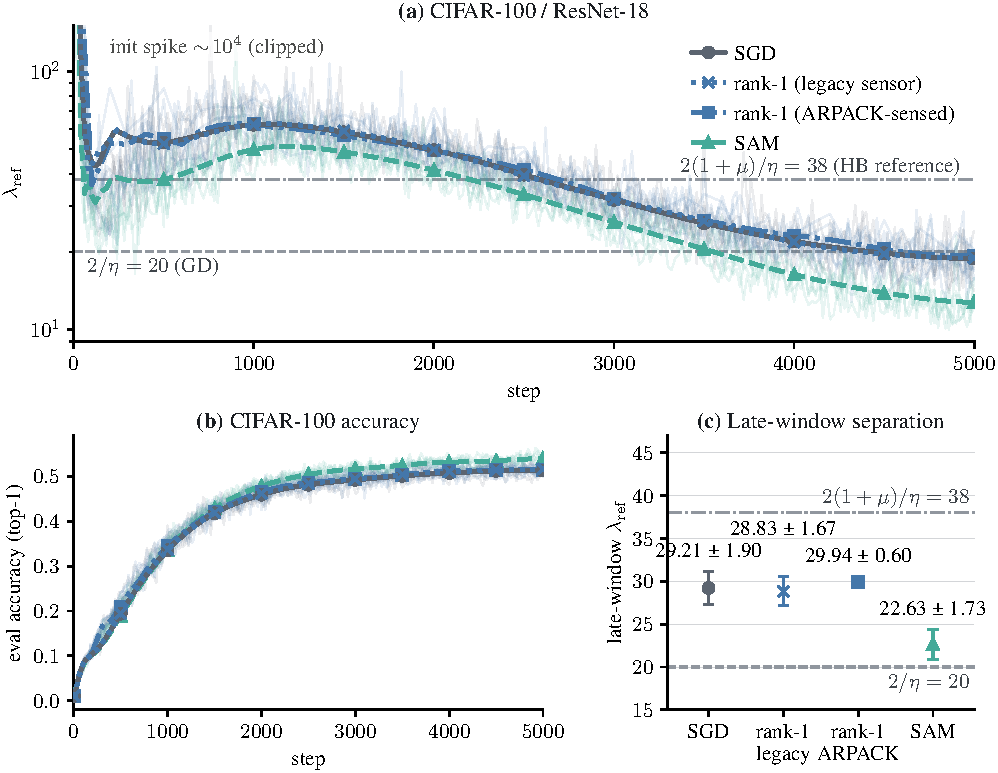
\includegraphics[width=0.95\linewidth]{30_cifar100_r18_control.pdf}
\caption{规模复现：ResNet-18（11.2M）/CIFAR-100，确定性 CUDA，ARPACK 在
确定性 512 样本评估批上测 $\lmax$（$n=5$ 种子）。\textbf{(a)} $\lmax$
轨迹（细线为各 seed、粗线为均值；y 轴截断在 $150$——初始化瞬态
（transient，系统进入稳定模式前的短暂过渡阶段；训练开始时 $\lmax$
冲到 ${\sim}10^{4}$ 的尖峰即瞬态，不代表长期行为）尖到
${\sim}10^{4}$），同时画出 GD 边界 $2/\eta=20$ 与起作用的重球边界
$2(1+\mu)/\eta=38$。\textbf{(b)} 评估精度。\textbf{(c)} 晚窗口（步
$\ge2000$）$\lmax$ 均值 $\pm95\%$ CI：$\{\text{SGD}\approx\text{rank-1}\}$、
SAM 在其下方、CI 不重叠。图中 rank-1 plant 是被钳位的 C3 变体：其自门控
钳位使它在此休眠（触发比例 $\le4\%$，源于下述感知伪收敛，并非体制属性）；
修正后的 ARPACK 感知 plant 以全力开火却仍对尖锐度无影响（有动作仍被钉住，
$n=5$，见 \S\ref{sec:ch08-pinned}）。}
\label{fig:ch08-r18}
\end{figure}

\subsection{方法论插曲：幂迭代伪收敛——proxy 坏了，不是体制坏了}\label{sec:ch08-falseconv}

这一小节是全章最重要的方法论叙事，值得慢慢读。

\textbf{发生了什么。}原版 rank-1 plant 用小批幂迭代估计顶部特征向量，并把
阻尼门控在 $\hat\lambda>2/\eta$ 上。在 ResNet-18 上它读到
$\hat\lambda\approx19<2/\eta=20$，于是只在 $\le4\%$ 的步上触发
（$\approx$SGD）。最初的解读是：“批尖锐度就坐在 $2/\eta$ 上”。

\textbf{ARPACK 直测推翻了这个解读。}在确定性 512 样本批上，顶部特征值其实
是 $\lmax\approx36$（中位 $35.7$、训练全程均值 $40.5$、$88\%$ 的步高于
$2/\eta=20$）。那个 $\approx19$ 是\emph{幂迭代伪收敛}（false
convergence）：两次 HVP 后的早停落在了\emph{次主导瑞利商}上，平均低估
$+45\%$。一句话：\emph{proxy 坏了，不是体制坏了}——随机 EoS 体制本来
好好的，坏的是那个廉价传感器。

这里有一个普适教训，与第~\ref{sec:ch10}~章的“监测器”建议相接：近简并的
重尾谱（近简并 = 前几个特征值几乎相等、“谁是最尖方向”难分伯仲——
此时幂迭代分不清该收敛给谁；重尾 = 除少数极大特征值外、大量方向仍有
可观的曲率；这是 ResNet-18 海森的典型谱形）正是 warm-start 幂迭代最脆弱的环境；当你的
廉价 proxy 读出一个“恰好支持你假设”的数字（“批尖锐度在 $2/\eta$”）时，
这个巧合本身就是值得怀疑的理由。论文的处置是换成确定性批 + ARPACK 直测，
并把测量协议写进结论。

\subsection{true-$\lmax$ plant：执行器真打了，尖锐度不动}\label{sec:ch08-pinned}

\textbf{修好感知。}论文把传感换成 warm-start ARPACK（$k=2$、
$\mathrm{tol}=10^{-2}$），每 $N=20$ 步在同一个确定性批上执行，并去掉原
plant 除数里的 $\max(\cdot,1)$ 下限。于是阻尼除数为
$\lmax/(2/\eta)\approx1.8$，秩-1 阻尼因子每步 $\approx0.44$（即除数蕴含
的瞬时每步因子 $1-1/d$；后文的 $0.46$、$0.39$ 与此同为 $1-1/d$ 的
不同口径——分别由中位除数 $1.86$ 与窗口均值得出，因 $d$ 逐步波动
而略有出入）。

\textbf{预注册（pre-registered，实验前公开承诺合格判据——防止看完
结果再临时改标准、把噪声解读成胜利）合格判据。}主除数判据（中位 $1.86$，门槛 $\ge1.5$）与阻尼
均值判据（每步阻尼的窗口均值实现值 $+0.39$，门槛 $>0.3$）在全部 $n=5$ 个
确定性种子上达标，Ritz 有效力率 $100\%$（以 Ritz 残差判定“传感读数
仍新鲜有效”的步数占比——残差合格说明执行器动用特征向量估计时该估计
未过期，无陈旧性混淆）。辅助的触发率
判据被透明报告：它\emph{没有}在全程 5000 步窗口达标（$83\%$，低于预注册
的 $95\%$），但在实质训练窗口（步 1--4000）内达标（$98.5\%$）。注意
判据的分级：除数与阻尼两条是预注册的\emph{主}判据（成功标准）且已
全部达标；触发率只是``动作在场''的辅助监测而非成功标准，其晚期下滑
有机制解释并被如实披露——不是事后改标准。晚期下探
是``动作起效''而非``动作缺席''：执行器在晚期把 $\lmax$ 拉向目标
$\lambda_{\mathrm{targ}}$，除数\emph{按设计}跌破触发阈值——动作成功的
副作用，不是动作缺席。

\textbf{结局：有动作仍被钉住。}执行器确实在打（除数 $\approx1.8$、每步
阻尼因子 $\approx0.44$），可尖锐度轨迹几乎不动：$\lmax$ 稳态中位数
$[37.2,36.9,39.7,35.6,36.3]$（五个种子）与 vanilla SGD（$33.8\pm3.7$
——此基线为 true-$\lmax$ plant 实验族的伴随 SGD 臂，口径是稳态中位
数的跨种子统计，与表~\ref{tab:ch08-threeway} 的晚期均值口径不同，
故数值有差）重叠。以真实力阻尼\emph{一个}方向钉不住高秩谱：尖锐度在秩-$(n{-}1)$
正交补上重新分布，并且无论阻尼与否都绕当下体制的实际阈值（重球边界
$38$）自稳定。这就是
预测器$\ne$执行器二分的规模版——\emph{有动作仍被钉住}（pinned
despite action）：执行器可验证地全力开火，$\lmax$ 却不出跨种子噪声包络。
它与全批 MLP 体制恰好相反：在那里，同样精确的执行器会上逃逸到
$261.8\pm5.4$（第~\ref{sec:ch09}~章给出两种体制的统一理论视角）。只有
全局动作能降到阈值以下——SAM 同时作用于每个方向。

\subsection{更长日程的外部效度：12000 步 + 标准增强}\label{sec:ch08-long}

5000 步、恒定学习率、无增强是一个欠拟合体制（underfitting regime，模型尚未学满、离峰值精度还远；第~\ref{sec:ch10}~章的局限
(vii)）。为探测排序的外部效度，论文在 12000 步（${\approx}31$ epochs）+
标准 pad/crop + 水平翻转增强下重跑三向（$n=2$ 种子/臂，同一确定性 +
ARPACK 协议）。晚窗口（步 $\ge8000$）$\lmax$：SGD $21.9$、rank-1
$22.8$、SAM $18.1$。三个观察：

\begin{itemize}
  \item SAM 甚至低于 \emph{GD} 边界 $2/\eta=20$；
  \item rank-1 plant 与 SGD 差 ${\sim}1$ 单位（有动作仍被钉住）；
  \item 排序 $\text{SAM}<\{\text{SGD}\approx\text{rank-1}\}$ 不变（逐种子
        差距符号一致，SAM-vs-SGD 为 $-3.4/-4.2$）。
\end{itemize}

SAM 同时拿到最好精度（$0.68$ vs $0.66$）；增强把每一臂都抬高了——作为
参照，5000 步无增强的 CIFAR-100 精度只有 ${\sim}52\%$。

\subsection{ResNet-18 上的 rank-$k$：null 结果，不是第二次机制反驳}\label{sec:ch08-rankk}

rank-$k$ 扫描（$k=1,2,5$，原幂迭代感知 plant）在 ResNet-18 上是平的：
$k=1$：$30.29\pm1.45$、$k=2$：$32.25\pm5.72$、$k=5$：$34.06\pm4.52$
（各 $n=5$）——在该协议下都 $\approx$SGD（ARPACK 测的 $k=1$，即
$28.83\pm1.67$，就是上面三向中的 rank-1；换用 ARPACK 后绝对值有偏移，
$k$-不变结论不变）。此处要分清\emph{两把尺子}：前述``$+45\%$ 低估''
指 plant \emph{内部传感}的两次-HVP 早停止读数（$\hat\lambda\approx19$
vs ARPACK 真值 $\approx36$）；而扫表报告的 $\lmax$ 轨迹来自另一套
结局测量协议——两者不是同一把尺子，故表中幂迭代读数与 ARPACK 只差
约 $1.5$ 单位。

关键在于如何\emph{归因}这个 null：那个 plant 恰恰因 \S\ref{sec:ch08-falseconv}
记录的感知伪收敛而休眠；修正的 true-$\lmax$ $k=1$ plant \emph{确实}开火，
却仍与尖锐度无关（有动作仍被钉住），所以 null 只会\emph{更}成立：任何
$k$ 都没有下逃逸。但论文明确说：这是\emph{控制性}结果，\emph{不是}对“谱
迁移”备择的第二次独立反驳——那次反驳要靠 MLP 多尖锐景观测试（在那里执行
器确实触发、$k$ 确实要紧，见第~\ref{sec:ch09}~章的逐方向结构）。这里只主张
rank-$k$ 的\emph{排序}结论——无 $k$ 下逃逸、唯 SAM——在真实 CNN 上成立。
（``控制性结果''指该实验的作用只是排除“plant 休眠所以测不出”这一干扰
解释、从而加固已有结论，并不提供一条新的独立证据线；独立反驳需要专门
设计的新实验，如 MLP 多尖锐景观测试。）

\subsection{为何 SAM 能而秩-1 不能（实证侧）}\label{sec:ch08-why}

论文 \S5.7 末段给了一个统一的透视：两者的对比不是“局部 vs 全局几何”，而是
\emph{方向性动作 vs 曲率感知动作}作用于同一景观。

SAM 的扰动先把梯度查询点移到
$\theta+\rho\nabla L/\|\nabla L\|$ 再求梯度；一阶展开（Andriushchenko 等人，2022）
显示这给更新加上 $(\rho/\|\nabla L\|)\,H\nabla L$，于是顶部方向被一个
\emph{曲率相关}因子 $1+\rho\lambda_{1}/\|\nabla L\|>1$ 放大——尖锐轴上的
有效步长\emph{变大}，SAM 所追踪的稳定性边界相应\emph{下移}到 $2/\eta$ 之下
（Long 等人，2024）。秩-1 阻尼做的是相反的事：顶部方向被缩到 $1/d<1$，
有效步长变小、边界\emph{上移}到 $y^{*}>0$（形式化见第~\ref{sec:ch09}~章
的命题 1 与两条推论）。两个执行器朝相反方向移动 EoS 阈值；只有曲率放大
型（全方向）的那个到达下逃逸区。

最后校准期望：SAM-vs-其余的分离幅度在 CIFAR-100 三向里 ${\sim}7$ 单位、
在 CIFAR-10 的 X-SAM 设定里 ${\sim}8$、在 MLP 头条里 ${\sim}19$。小批噪声
与动量模糊了分离——所以规模上的复现是\emph{定性}的（排序 + CI 分离），
不是 GD 体制那种精确的 $2/\eta$ 钉住。

\subsection*{本章要点}
\begin{itemize}
  \item 三向对比在 ResNet-18/CIFAR-100（$n=5$、确定性 CUDA + ARPACK）复现
        为\emph{双结局}：$\{\text{SGD}\approx\text{rank-1}\}$ vs SAM
        （$22.63\pm1.73$，CI 不重叠），且多数晚期步低于重球边界 38
        （frac${}<38$：$81\%/82\%/94\%$），与随机 EoS 一致。
  \item 原 plant 的“$\hat\lambda\approx19$、$\le4\%$ 触发”是幂迭代伪
        收敛：ARPACK 直测 $\lmax\approx36$（中位 $35.7$、均值 $40.5$、
        $88\%$ 步 $>20$），$\approx19$ 是落在次主导瑞利商上的 $+45\%$
        低估——proxy 坏了，不是体制坏了。
  \item true-$\lmax$ plant（ARPACK，$k=2$、tol $10^{-2}$、每 $20$ 步、无
        钳位下限）全力开火（除数中位 $1.86$、每步阻尼 $\approx0.44$、
        Ritz 有效力率 $100\%$），$\lmax$ 稳态仍与 SGD 重叠——规模版的
        \emph{有动作仍被钉住}。
  \item 12000 步增强日程保序（SAM $18.1<$ SGD $21.9\approx$ rank-1
        $22.8$；SAM 精度最好 $0.68$ vs $0.66$）；ResNet-18 rank-$k$ 是
        null 而非第二次机制反驳（机制反驳靠 MLP 多尖锐测试）。
  \item SAM 与秩-1 阻尼朝相反方向移动 EoS 阈值：曲率放大因子
        $1+\rho\lambda_1/\|\nabla L\|>1$ 下移边界，$1/d<1$ 上移边界——
        形式化在第~\ref{sec:ch09}~章。
\end{itemize}

% ============================================================
% ch09：理论解读：自稳定帽（对应论文理论附录 self_stabilization_cap.tex）
% 读者已读 tutorial/（含 Damian 定性图像）；本章升级为 2-D 递推定量图像。
% ============================================================

\section{理论解读：自稳定帽}\label{sec:ch09}

\begin{keybox}{本章速览}
\begin{itemize}
  \item Damian 二维递推的周期-2 不动点 $|x|{\to}\delta=\sqrt{2\alpha/\beta}$
        把 $S=\lmax$ 钉在 $2/\eta$：\emph{帽就是振荡本身}——教程第 7 节
        定性故事的定量骨架。
  \item 秩-1 阻尼后的均衡超出量 $y^{*}=2\gamma/((1-\gamma)\eta)>0$ 且随
        $\gamma$ 单调升：阻尼搬走的是帽的高度（向上），不是振荡的振幅
        $|x^{*}|=\sqrt{2\alpha/\beta}$。
  \item 命题（转述自论文 Proposition 1）：翻号周期-2 轨道\emph{没有}
        $y^{*}\le0$ 的；条件 $y$-收缩乘子 $\mu_y=1-\kappa$
        （$\kappa=2(1-\gamma)\eta^2\alpha$），$|\mu_y|<1\iff
        (1-\gamma)\eta^2\alpha<1$。
  \item 两条推论划边界：SAM 的曲率放大型全局动作把边界压到
        $\lambda^{*}_{\mathrm{SAM}}<2/\eta$（下逃逸）；缩放型单方向动作
        只能上移边界（上逃逸）或留帽。缺口 G1--G5 在案：这是二维约化
        定理，不是轨迹定理。
\end{itemize}
\end{keybox}

\begin{notebox}[title={动力系统小词典：本章的专用词汇（第 0 章背景速查 D 组的精简版）}]
\begin{itemize}
  \item \textbf{不动点}：迭代一步后原地不动的状态（类比 loss 收敛到的
        驻点）。\textbf{周期-2 轨道}：两个点轮流切换、每两步一循环的
        迭代序列——学习率偏大时 loss 在两个值之间来回跳即此物。记号
        $F^{2}$ 表示把更新规则 $F$ \emph{复合执行两步}（不是平方），
        于是“周期-2 轨道”就是 $F^{2}$ 的不动点；
  \item \textbf{均衡 / 稳态}：训练动力学的长期驻留模式。本章的均衡
        \emph{不是静止点}，而正是那条周期-2 振荡轨道；“$\lmax$ 钉在
        $2/\eta$”即曲线长期停在阈值附近来回振荡；
  \item \textbf{翻号}：迭代每步改变符号（$x\to-x$）；\textbf{ansatz /
        试解}：先猜解的形状（如“每步变号、幅度不变”）代回方程验证；
  \item \textbf{线性稳定性分析 / Jacobian}：在均衡附近把更新规则做
        一阶泰勒展开，得一阶导数矩阵（Jacobian，小扰动每步被如何
        放大/旋转的局部线性近似）；其特征值的模 $>1$ 表示扰动被放大
        （不稳定）、$<1$ 表示被吸住（收缩）；
  \item \textbf{乘子}：给周期轨道一个小扰动，绕轨道一整圈后扰动被乘
        的系数；$|\mu|<1$ 即该方向扰动每圈缩小。\textbf{排斥子}：附近
        轨道被推离的状态（吸引子的反面）——轨道“是排斥子”不妨碍
        实验观察到它：真实轨迹可在排斥轨道\emph{附近}贴着走；
  \item \textbf{慢--快结构}：系统里同时有每步剧变的快变量与每步只挪
        一点的慢变量；奇异摄动即“近似认为快变量瞬时到达均衡、把耦合
        问题拆成两个一维问题”的标准方法。\textbf{快流形}：慢变量
        冻结时快变量走出的轨道；\textbf{役使}：快变量被慢变量锁死、
        只能瞬时跟随；\textbf{不变图}：迭代进入后不再离开的点集
        （这里是 $x\in\{\pm x^{*}\}$ 两点循环）。
\end{itemize}
\end{notebox}

\textbf{本章在论文中的位置。}论文把控制端的负结果陈述为“机制猜想”
（Claim 1，非正式），完整理论化在附录 \texttt{self\_stabilization\_cap.tex}：
启发式（阻尼后的二维递推）、形式化命题（带稳定性分析）、两条推论、一个
观察与缺口清单 G1--G5。本章按同样顺序转述，重心放在\emph{每个公式的
直觉}：这个阻尼的\emph{定量}形式是什么？用执行器去碰它会发生什么？
这个理论\emph{不}主张什么？

\subsection{从定性故事到定量骨架：Damian 二维递推}\label{sec:ch09-damian}

教程第 7 节讲过：$\lmax$ 越过 $2/\eta$ 后，GD 沿顶部特征向量（教程记
$\vtope$，本章按论文记 $u_1$）做周期-2 振荡，三阶泰勒项的阻尼
把 $\lmax$ 拉回来。Damian 等人 (2023) 把它写成二维递推，支点是恒等式
\begin{equation}
  \nabla S \;=\; \nabla^{3}L(u_1,u_1),
  \label{eq:ch09-identity}
\end{equation}
其中 $S(\theta)=\lmax(H)$：\emph{尖锐度的梯度就是三阶张量在顶部方向上取
两次的收缩}。直觉：沿 $u_1$ 移动 $x$，曲率以
$\nabla^{3}L(u_1,u_1)\cdot x$ 的速率变化——振荡不仅“移动参数”，还直接
“改写谱”。状态变量：$x_t$ 是迭代点沿 $u_1$ 的位移；$y_t=S-2/\eta$ 是
相对阈值的\emph{超出量}；$\alpha=-\nabla L\cdot\nabla S>0$ 是\emph{渐进
尖锐化系数}（每单位移动供给多少尖锐度）；$\beta=\|\nabla S\|^2$。于是
\begin{equation}
  x_{t+1}=-(1+\eta y_t)\,x_t,
  \qquad
  y_{t+1}=y_t+\eta\!\left(\alpha-\tfrac{\beta}{2}x_t^{2}\right).
  \label{eq:ch09-damian}
\end{equation}
\textbf{逐项直觉。}$x$-方程是沿顶部方向的线性化 GD：系数 $-(1+\eta y)$
在 $y>0$（不稳定区）模大于 $1$，每步\emph{翻号并放大}（sign-flip，每步改变符号的振荡）——周期-2 振荡的
生成器。$y$-方程是慢漂移：每步加 $\eta\alpha$ 的尖锐化供给，减去
$\tfrac{\beta}{2}x^2$ 的\emph{三次恢复力}——“三次”指它源自泰勒展开的
三阶项（曲率对位置的变化率，由恒等式
\eqref{eq:ch09-identity} 给出），对 $y$ 的增量恰是位移的\emph{二次}式：
大幅振荡直接改变曲率，振幅越大、恢复力越强。
令放大停止（$y\to0$）且 $y$-增量归零，得周期-2 不动点：
\begin{equation}
  |x|\;\to\;\delta=\sqrt{2\alpha/\beta},
  \qquad
  y\to0\;(S\approx2/\eta).
  \label{eq:ch09-fixedpoint}
\end{equation}
直觉读法：$\alpha$ 是“每步打进来的尖锐度预算”，$\tfrac{\beta}{2}x^2$
是“振荡用振幅换来的曲率回撤”，预算平衡决定振幅。$2/\eta$ 不是外部强加
的约束，而是这个自洽解（自洽 = 解的取值反过来支撑解自身成立）的值——
\emph{帽（cap）就是振荡本身}。这也是后文“均衡”一词的确切所指：不是
静止点，而是这条振幅 $\delta$、尖锐度 $\approx2/\eta$ 的周期-2 驻留
轨道。伏笔由此埋
下：想移除帽就必须移除振荡；想保留振荡，帽就在。

\subsection{论断（转述自论文 Claim 1）：秩-1 阻尼的两种命运}\label{sec:ch09-claim}

\begin{claim}[秩-1 阻尼无法下逃逸；非正式，转述自论文 Claim 1]
秩-1 执行器干预（plant action，直接改写梯度）把梯度沿 $u_1$ 的估计
$\hat v$ 方向的分量阻尼掉。它有两种命运，都不下逃逸：
\begin{itemize}
  \item \emph{不完美阻尼}（$\hat v$ 滞后于 $u_1$，如自由的
        $\hat v=\Delta\theta_{t-1}/\|\cdot\|$）：平行梯度分量的抵消不
        完全，周期-2 振荡持续，自稳定帽保持，$\lmax$ 钉在 $2/\eta$。
  \item \emph{精确阻尼}（$\hat v\approx u_1$，如幂迭代）：抵消趋于精确
        （$\eta_{\mathrm{eff}}\lambda_1\to2$），周期-2 振荡被
        \emph{解除武装}，帽被移除，渐进尖锐化无阻进行——$\lmax$ 长过
        $2/\eta$（上逃逸），而不是低于它。
\end{itemize}
只有\emph{全局}执行器干预（SAM，其扰动作用于每个方向）能下逃逸。
\end{claim}

实证锚点（论文控制实验，实证侧见第~\ref{sec:ch08}~章）：自由 $\hat v$
锁定 $40.12\pm0.12=2/\eta$；精确 $\hat v$（$k=1$）上逃逸到
$261.8\pm5.4$ 且 $k=1,2,5,10$ 逐位相同（一维尖锐谱
$\lambda_2\approx0.6$）；多尖锐景观上每方向独立上逃逸（${\sim}65$）；
SAM 逃到 $21.35\pm0.04<2/\eta=40$，而忠实 X-SAM 消融（$n=10$）里其
秩-1 修正每步开火、晚期效应量上界仅 $+1.85$。

\subsection{阻尼后的 $x$-递推：帽被搬到哪里？}\label{sec:ch09-damped}

执行器把梯度改写为
\begin{equation}
  g' = g-\gamma\,(g^{\!\top}\hat v)\,\hat v,
  \qquad
  \gamma=1-\tfrac{1}{d}\in(0,1),
  \qquad
  d=\max\!\bigl(\hat\lambda/(2/\eta),\,1\bigr),
  \label{eq:ch09-edit}
\end{equation}
即把 $\hat v$ 方向的梯度分量乘以 $1/d$（除数由感知尖锐度的超阈值倍数
自门控）。取 $\hat v\approx u_1$、窗口内 $d$ 固定，位移递推变为
\begin{equation}
  x_{t+1}=\bigl(1-(1-\gamma)\eta\lambda_1\bigr)x_t
         =\bigl(-1+2\gamma-(1-\gamma)\eta y_t\bigr)x_t,
  \label{eq:ch09-damped-x}
\end{equation}
$y$-递推保持 \eqref{eq:ch09-damian} 的形式（第二个等号用了
$\eta\lambda_1=2+\eta y$：$\gamma=0$ 时回到 Damian 映射——单参数形变，
即同一递推拧“阻尼强度 $\gamma$”一个旋钮得到的连续变形版本）。
代入周期-2 试解（$x_{t+1}=-x_t$，翻号 ansatz）：
\begin{equation}
  y^{*}=\frac{2\gamma}{(1-\gamma)\eta}\;>\;0,
  \qquad
  |x_*|=\sqrt{2\alpha/\beta},
  \label{eq:ch09-ystar}
\end{equation}
后者由 $y$-方程在轨道上增量为零给出。三条读法：\textbf{符号}，
$y^{*}>0$——精确阻尼把均衡移到阈值\emph{上方}，与控制目标相反。直觉：
阻尼调低翻号放大器的增益（gain，放大倍数——即每步把信号乘多大的那个
系数），而 $y=0$ 处增益恰为 $-1$（等幅翻号）；要恢复
等幅翻号，必须让 $y$ 升高、用更大的“本征不稳定”补回被除掉的放大。
\textbf{单调性}，$\partial y^{*}/\partial\gamma=2/((1-\gamma)^2\eta)>0$
——阻尼越强，均衡尖锐度越高。\textbf{振幅不变}，$|x_*|=\sqrt{2\alpha/\beta}$
与无阻尼时逐字相同——$y$-方程的预算平衡不含 $\gamma$；阻尼改变“帽的
高度”，不改“振荡的幅度”，帽被搬走了，但搬\emph{向上}。

\subsection{启发式预测什么、不预测什么}\label{sec:ch09-heuristic}

论文对 \eqref{eq:ch09-ystar} 的定位非常克制。\textbf{它预测的：}符号
（向上）与参数依赖——均衡 $S^{*}=2/\eta+y^{*}=2d/\eta$；已被精确
$\vtope$ 实验确认（一维尖锐景观上逃逸 $261.8\pm5.4$，多尖锐
景观 ${\sim}65$）。\textbf{它不预测的：}逃逸\emph{量级}——自门控
$d=\hat\lambda/(2/\eta)$、$\gamma=1-1/d$ 下，把 $d$ 代回
\eqref{eq:ch09-ystar}，条件化为恒等式 $y^{*}=y$，\emph{任何}
$\lambda_1>2/\eta$ 都满足不动点条件；至于上方多远，由无阻碍渐进尖锐化
在哪里平衡决定（四次及更高阶景观项的事）——$261.8$ 不是理论预测值，
是景观的属性。\textbf{它不涵盖的：}自由滞后 $\hat v$ 根本\emph{不进入}
该推导——$\hat v\not\approx u_1$ 时 $\hat\lambda$ 读次主导轴、自门控
$d$ 被错误曲率设定，而 \eqref{eq:ch09-damped-x} 瞄准的 $u_1$-振荡基本
未被触碰，帽保持。Claim 1 的两种体制由此统一为“推导前提是否成立”：
精确 $\hat v$ 进入 $y^{*}>0$ 体制；滞后 $\hat v$ 从未真正作用到 $u_1$
轴上。

\subsection{命题（转述自论文 Proposition 1）：翻号周期-2 轨道不低于阈值}\label{sec:ch09-prop}

设 $F$ 为 \eqref{eq:ch09-damped-x} 与 \eqref{eq:ch09-damian} 之 $y$-方程
定义的二维映射。三个假设：

\begin{assumption}[A1：非退化顶部对，转述]
$(\lambda_1,u_1)$ 沿轨迹简单且孤立（“简单”即该特征值没有并列——只
对应一个特征方向；“孤立”即与第二名拉开 $\lambda_1-\lambda_2\ge\Delta>0$
的距离，否则“谁是最尖方向”不唯一），$\lambda_1-\lambda_2\ge\Delta>0$，
故 $\nabla S$ 良定义（良定义 = 无歧义地存在：$\lmax$ 无并列时 $S$
才是参数的光滑函数、梯度才存在，Damian 等人 2023 的引理 2 需要 $\lmax$ 简单）。
\end{assumption}

\begin{assumption}[A2：窗口固定阻尼，转述]
$\gamma\in(0,1)$ 在分析窗口内常数（它在 $O(1/\eta)$ 步上演化；
$x$-动力学是 $O(1)$ 的——慢-快尺度分离）。
\end{assumption}

\begin{assumption}[A3：精确感知，转述]
$\hat v=u_1$（理想化；任何感知误差只会减弱阻尼）。
\end{assumption}

\begin{proposition}[秩-1 阻尼无法下逃逸；转述自论文 Proposition 1]
在 A1--A3 下，对 $\alpha,\beta,\eta>0$、$\gamma\in(0,1)$：
\begin{itemize}
  \item[(a)] \emph{代数部分。}$F$ 的每个\emph{翻号}周期-2 不动点——
        $F(x_*,y_*)=(-x_*,y_*)$、$|x_*|>0$，即每步把位移翻号、走两步
        恰好回到原处的两步循环——都满足
        $y^{*}=2\gamma/((1-\gamma)\eta)>0$ 且
        $|x_*|=\sqrt{2\alpha/\beta}$；\emph{不存在} $y^{*}\le0$ 的翻号
        周期-2 轨道。（$F^2$（复合执行两步的映射）在 $\kappa>4$ 时还容许\emph{非翻号}周期-2
        轨道，$y$ 在两个负值间交替，但要求 $y<-2/\eta$ 即 $S=\lmax<0$，
        与 A1 矛盾——以\emph{物理性}（数学解必须满足的现实约束，此处即
        “最大特征值非负”）而非稳定性排除，因为命题分析的翻号
        轨道本身就是全映射排斥子（附近轨道被推离的状态），稳定性不能作为区分两族轨道的判据。）
  \item[(b)] \emph{条件 $y$-收缩（conditional $y$-contraction，仅在
        “$x$ 保持在周期-2 轨道上”这一前提下成立的自发收缩：$y$ 的扰动
        两步后乘以 $\mu_y$ 变小；它不等于轨道稳定——整体上轨道仍被
        排斥，见 \S\ref{sec:ch09-remarks}）。}令
        $\kappa:=2(1-\gamma)\eta^2\alpha>0$，则\emph{在 $x$ 保持周期-2
        轨道这一条件下}的两步 $y$-方向乘子（multiplier，绕周期轨道一
        圈后小扰动被乘的系数，$|\mu|<1$ 即扰动每圈缩小）为 $\mu_y=1-\kappa$，满足
        $|\mu_y|<1$ 当且仅当 $(1-\gamma)\eta^2\alpha<1$。这是不变图（invariant graph，迭代映射进入后不再离开的点集——这里即
        $x\in\{\pm x_*\}$ 两个点来回跳的集合；“图”是动力系统对“由
        状态参数化的集合”的称呼，与神经网络计算图无关）
        $x\in\{\pm x_*\}$ 上慢方向的收缩（收缩此处=缩小；与张量的
        ``收缩/缩并''重名不同义），\emph{不是}轨道稳定性结果
        （全二维映射正常排斥——完整二维映射在所有方向把附近轨道推开，
        见 \S\ref{sec:ch09-remarks}；轨道稳定性
        还需 G4 的高阶 $|x|$-界）。
\end{itemize}
\end{proposition}

\textbf{证明思路（直觉版）。}(a) 是纯代数：翻号试解代入
\eqref{eq:ch09-damped-x}、消去 $x_*$ 即得 \eqref{eq:ch09-ystar}；$y$-方程
两步增量为零给出振幅。(b) 用慢-快/奇异摄动（slow--fast analysis / singular perturbation，系统里同时有每步剧变的快变量与每步只挪一点的慢变量时的标准分析方法：近似认为快变量瞬时到达均衡、把耦合问题拆成两个一维问题——类比把“每个 step 的高频震荡”与“几千步的缓慢漂移”分成两层）分析：$y$ 慢（每步漂移
$O(\eta)$，即与学习率同量级的小幅度）、$x$ 快（每步翻号）。记 $m(y)=-1+2\gamma-(1-\gamma)\eta y$
（故 $m(y^*)=-1$），扰动 $y\to y^{*}+\varepsilon$ 且 $x$ 留在快流形（快变量在慢变量暂时冻结时走出的那条轨道）：
第一步给 $x_1=(-1-(1-\gamma)\eta\varepsilon)x_*$、$y_1=y^*+\varepsilon$
（$y$-增量因 $|x_*|=\sqrt{2\alpha/\beta}$ 消失）；第二步用
$x_1^2=(1+2(1-\gamma)\eta\varepsilon)x_*^2+O(\varepsilon^2)$ 与
$\beta x_*^2=2\alpha$，得
\begin{equation}
  y_2 = y^{*}+\varepsilon-\underbrace{2(1-\gamma)\eta^2\alpha}_{=\,\kappa}\,\varepsilon
  +O(\varepsilon^2)
  = y^{*}+(1-\kappa)\,\varepsilon+O(\varepsilon^2).
  \label{eq:ch09-contraction}
\end{equation}
\textbf{直觉读法}：$\kappa$ 是“恢复力对超出量的回拉增益”。$y$ 超调
$\varepsilon$ 后，$x$-放大器先放大一点（第一步），更大的振幅产生更强的
三次恢复力（第二步），把 $y$ 往回拉 $\kappa\varepsilon$；回拉不失控
（$\kappa<2$，即 $|\mu_y|<1$ 的等价形式）即慢方向收缩——$\kappa<1$
时单调回拉，$1\le\kappa<2$ 时回拉过零翻号但每圈仍在缩小。$(1-\gamma)\eta^2\alpha<1$（即 $\kappa<2$）是“阻尼不太强、
学习率不太大、渐进尖锐化不太猛”的组合——典型 EoS 体制都安稳处于其中。

\subsection{三个注记：命题\emph{不}主张什么}\label{sec:ch09-remarks}

\begin{remark}[退化与不稳定不动点在范围外，转述自论文 Remark]
$F$ 还有退化周期-1 不动点（周期-1 = 走一步即回到原处，就是不动点本身；
``退化''指其振幅为零的平凡临界情形——与特征值的``简并''重名不同义）
$y=-2/\eta$（$S=0$），在 EoS 体制之外。更
值得留意的是 $(1-\gamma)\eta^2\alpha\ge1$（即 $\kappa\ge2$）时
$|\mu_y|\ge1$，均衡连\emph{条件}稳定也失去——可能是“强阻尼 + 强渐进
尖锐化”下最剧烈上逃逸的路径；论文实验（$\eta=0.05$、中等 $\alpha$）
安稳处于 $\kappa<1$。
\end{remark}

\begin{remark}[体制（i）在命题前提之外，转述自论文 Remark]
A3 把命题放进体制（ii）（精确感知）。体制（i）（滞后/自由 $\hat v$）下
感知方向漂离 $u_1$，有效阻尼变为
$\gamma_{\mathrm{eff}}=\gamma\cos^2\varphi$（缺口 G5）；极限
$\hat v\perp u_1$ 时 $u_1$-振荡完全未被触碰、帽保持 $2/\eta$。体制
（i）\emph{不是}命题的反例，而是其前提\emph{从未生效}的体制——迭代点
默认坐在无阻尼均衡 $y^{*}=0$ 上。
\end{remark}

\begin{remark}[全二维 Jacobian：命题只主张条件 $y$-收缩，转述自论文 Remark]
$DF^2$（映射 $F$ 复合两步后的一阶导数矩阵，即 Jacobian——小扰动每步
被如何放大/旋转的局部线性近似；特征值的模 $>1$ 表示扰动被放大）在 $(x_*,y_*)$ 处特征值为 $(1-\kappa)\pm2i\sqrt{\kappa}$（一对共轭
复特征值——小扰动可以``边转边缩''，旋转分量在数学上记成虚部 $i$；
``模'' = $\sqrt{\text{实部}^2+\text{虚部}^2}$，即总的放大倍数）、模
$1+\kappa>1$：全二维映射\emph{正常排斥}（在所有方向上把附近轨道推开
——但真实轨迹仍可在排斥轨道\emph{附近}贴着走，所以理论不稳定不等于
实验上看不见）。命题 (b) 只主张\emph{条件}
$y$-方向乘数（不变图 $x\in\{\pm x_*\}$ 上、$x$ 被役使——役使即快变量
被慢变量锁死、只能瞬时跟随而无独立动力学），不主张渐近
稳定性（渐近稳定 = 从附近出发的轨迹最终都收敛到该状态）。标准 EoS 直觉——快方向 $x$ 的放大充当“幅度伺服”（amplitude servo，伺服即
“持续把某个量拉回目标值”的闭环（闭环 = 边测边调、测量结果反馈进
下一步决策的回路）装置，恒温器是最常见的例子；此处指
振荡幅度自动充当恒温器：$y$ 超调
$\to|x|$ 增长 $\to$ 恢复力 $\beta x^2/2$ 压过渐进尖锐化 $\alpha$ $\to$
$y$ 被压回）——是缺口 G4 的\emph{猜想式}闭合：给 $|x_\infty|$ 定界需要
二维约化丢掉的四次及更高阶项。关键：负主张 (a) \emph{完全不依赖}这套
稳定性叙事，它是试解上的纯代数。
\end{remark}

\subsection{推论（转述）：向上逃逸只定方向；与 bulk 投影的会合}\label{sec:ch09-upward}

\begin{corollary}[向上逃逸，仅方向；转述自论文 Corollary]
均衡 $S^{*}=2/\eta+y^{*}=2d/\eta$（$d=1/(1-\gamma)$）；$\gamma\uparrow1$
驱动 $S^{*}\to\infty$。命题钉住\emph{方向}（$y^{*}>0$，向上）与参数
依赖（$S^{*}=2d/\eta$），但不钉住 $S$ 收敛到的有限值——那由无阻碍
渐进尖锐化在哪里平衡决定，超出二维约化的视野。
\end{corollary}

这使论文与 Song 等人 (2025) 接上头：他们把 SGD 更新投影到谱“bulk”
（去掉 top-$k$ 特征向量分量），报告尖锐度无约束增长而 loss 与精度保持。
在本文的视角下这正是 $\gamma\to1$（$d\to\infty$）极限：均衡 $S^{*}=2d/\eta$
随 $d\to\infty$ 发散，他们的“无约束增长”就是\emph{均衡本身的发散}。
“伪对齐”与“帽移除”两种解读描述的是同一条轨迹；只有后者定量预测 $\gamma$
依赖的发散。部分阻尼（$\gamma<1$）实验在有限 $S^{*}$ 处诊断帽；全投影
（$\gamma=1$）把它整个移除。

\begin{remark}[可分离多特征值扩展，转述自论文 Remark]
若 $H$ 可分离（$H=\sum_i\lambda_iu_iu_i^{\!\top}$、无非对角耦合——注意
谱分解这一步任何对称矩阵都有（海森天然对称：混合二阶偏导相等
$\partial^2L/\partial\theta_i\partial\theta_j=
\partial^2L/\partial\theta_j\partial\theta_i$），所以对海森永远合法；
``可分''额外限制的是\emph{高阶}交叉项为零：
动一个特征方向不会改变另一个方向的曲率，各方向动力学因此独立），
Damian 递推解耦为独立 $(x_i,y_i)$ 对，命题\emph{逐方向}成立：每个未
阻尼方向的帽留在 $y_i^{*}=0$、每个被阻尼方向移到 $y_i^{*}>0$。论文的
多尖锐景观测试在\emph{不可分}景观上实证确认了这种逐方向独立性——
Damian 等人 (2023) 留开放的情形——部分闭合缺口 G1。（按轨迹 PCA，第一
主成分解释 MLP/ResNet/ViT/ConvNeXt 轨迹方差的 84--99\%：一维尖锐几何
才是 EoS 的典型体制，多尖锐构造是诊断工具而非默认情形。）
\end{remark}

\subsection{推论（转述）：SAM 如何到达下逃逸区}\label{sec:ch09-sam}

\begin{corollary}[SAM 经曲率放大动作到达 $y<0$；转述自论文 Corollary]
SAM 的更新
$\theta_{t+1}=\theta_t-\eta\nabla L(\theta_t+\rho\nabla L/\|\nabla L\|)$
\emph{不进入}秩-1 递推 \eqref{eq:ch09-damped-x}：展开到 $O(\rho)$
（Andriushchenko 等人，2022），有效梯度
$\nabla L^{\mathrm{SAM}}\approx(I+\tfrac{\rho}{\|g\|}H)g$，把顶部方向
重缩放为 $1+\rho\lambda_1/\|g\|>1$（曲率\emph{放大}），从而把 SAM
追踪的稳定性边界降到
\begin{equation}
  \lambda^{*}_{\mathrm{SAM}}
  =\frac{\|g\|}{2\rho}\!\left(\sqrt{1+\tfrac{8\rho}{\eta\|g\|}}-1\right)
  <\frac{2}{\eta},
  \label{eq:ch09-sam-boundary}
\end{equation}
即 $y^{*}_{\mathrm{SAM}}<0$（Long 等人，2024）。秩-1 阻尼把顶部方向缩为
$1/d<1$（曲率\emph{衰减}），把边界抬到 $y^{*}>0$。这就是“全局动作
必要”的形式内容：只有曲率放大型（全方向）扰动到达下逃逸区；任何固定
预测方向上的秩-1 执行器都不能。
\end{corollary}

直觉：SAM 的扰动 $\rho g/\|g\|$ 一阶贡献 $(\rho/\|g\|)Hg$——沿 $g$
已有的分量按曲率加权加回去，顶部方向（曲率最大、且 EoS 对齐区里 $g$
本就偏向 $u_1$）被放得最猛：尖锐轴上有效步长变大，等价于 SAM 的稳定
运行点落在更低的尖锐度处。秩-1 阻尼是照镜子：同样的代数、符号相反
（第~\ref{sec:ch08}~章的 SAM $22.63\pm1.73$ vs rank-1 $28.83\pm1.67$
是规模版回声）。

\subsection{推论与观察（转述）：正交阻尼留帽；滞后无害}\label{sec:ch09-orth-lag}

\begin{corollary}[正交阻尼留帽；转述自论文 Corollary]
C4 执行器 $\Delta\theta=-\eta(g_{\parallel}+g_{\perp}/d)$（
$g_{\parallel}=(g^{\!\top}u_1)u_1$）\emph{保留}沿 $u_1$ 的梯度分量，其
$x$-递推因此就是无阻尼 Damian 映射 $x_{t+1}=-(1+\eta y_t)x_t$，周期-2
不动点 $y^{*}=0$：正交阻尼只重缩放补空间、不进入顶部方向动力学，对每个
$d$ 帽都保持 $2/\eta$。渐进尖锐化供给 $\alpha=-\nabla L\cdot\nabla S$
\emph{不}被重标（C4 保留 $g_{\parallel}$），误用
$y_{t+1}=y_t+\eta(\alpha/d-\beta x^2/2)$ 这类 ansatz 会把阻尼错误归因；
大 $d$ 时逐种子方差变宽是缺口 G4 的实测。
\end{corollary}

方法论教训：写错状态变量的 ansatz 也能解出“貌似合理”的均衡，把你引向
\emph{错误的机制归因}——推导必须逐项核对每个递推保留了一阶信息中的
哪些。

\begin{observation}[滞后无害；梯度方向探针钉住；转述自论文 Observation]
延迟更新传感器 $\hat v_k=\Delta\theta_{t-k}/\|\cdot\|$ 混淆两种缺陷——
\emph{滞后}，与使用更新（梯度）方向而非特征向量方向。分开后只有第二种
导致钉住：滞后\emph{但精确}的 $\hat v_k=\hat u(t-k)$ 留在体制（ii），
因为 $u_1$ 在慢的 $O(1/\eta)$ 时间尺度上旋转（Damian 等人，2023），
$\hat u(t-k)\approx u_1(t)$（只测短滞后 $k\le3$）。滞后的更新方向传感器
$\hat v_k=\Delta\theta_{t-k}\propto-g$ 则遭遇\emph{自致}感知失败：plant
自己的阻尼旋转更新方向 $\to$ 滞后 $\hat v$ 漂离 $u_1$ $\to$ 瑞利商崩塌
$\to$ 自门控钳位使 $\gamma=0$ $\to$ 退化为无阻尼 Damian GD、$y^{*}=0$。
起作用的是\emph{方向不精确}，不是\emph{数据陈旧}。
\end{observation}

帽对感知\emph{滞后}稳健、对感知\emph{不精确}不稳健：只有精确的顶部
方向感知才能实现帽移除（若无自门控钳位，陈旧瑞利商会翻转 $\gamma<0$、
反阻尼至发散——那是执行器病理，不是帽移除）。这把教程“必须用单步
$\Delta\theta$ 测对齐”的陷阱升级成执行器设计忠告：拿更新方向当传感器，
控制器会亲手毁掉自己的传感器。

\subsection{缺口清单 G1--G5：从二维定理到轨迹定理}\label{sec:ch09-gaps}

\begin{itemize}
  \item \textbf{G1（多特征值解耦）}。Damian 等人 (2023) 留给后续工作
        （其 \S8.2）的多特征值扩展仍开放；可分离情形已解
        （\S\ref{sec:ch09-upward} 注记），不可分情形有实证支持（多尖锐
        谱逐方向独立钉住）但无证明。
  \item \textbf{G2（旋转奇点）}。A1 在特征值交叉
        $\lambda_1\leftrightarrow\lambda_{j^*}$ 处失效（第二大特征值
        追平并反超最大值时，“哪个方向最尖”瞬间易主，尖锐度函数出现
        角点），$\nabla S$ 奇异（此处“奇异”指梯度无定义/爆炸，不是
        矩阵不可逆之义）；
        补丁开放（实证上轨迹以 $O(\eta^{-1})$ 步穿过交叉、定性结论
        保持）。
  \item \textbf{G3（时变 $\gamma$）}。扩展到分段常数 $\gamma_t$（刷新
        间隔 $N$）需扰动分析（perturbation analysis，把“每 $N$ 步才
        刷新一次”视为对理想连续情形的小偏差、用级数展开逐阶算出影响
        的数学方法，与 SAM 给参数加“扰动”无关）——这正是实际 plant 的运行方式（ResNet-18
        上每 $N=20$ 步刷新感知）。
  \item \textbf{G4（高阶 $|x|$-界）}。快方向放大需四次及更高阶景观项
        定界，二维约化没有它们；“幅度伺服”闭合仍是猜想。
  \item \textbf{G5（感知误差）}。$\hat v$ 与 $u_1$ 成角 $\varphi$ 时
        有效阻尼 $\gamma_{\mathrm{eff}}=\gamma\cos^2\varphi$，命题以
        $\gamma\to\gamma_{\mathrm{eff}}$ 保持。
\end{itemize}

清单之外，论文对框架隐喻也保持诚实：观测器-控制器分离原理
（observer--controller separation principle）在线性控制论里是精确的
定理，而这里的对象是非线性、非凸、（在规模实验里）随机且带动量的
动力学——连阈值本身都会移（全批 GD 的 $2/\eta$、重球的 $2(1+\mu)/\eta$、
随机 EoS 的批尖锐度阈值），所以控制端主张是\emph{机制猜想 + 二维约化
定理 + 三个控制实验}，不是轨迹定理。机制也依体制而变：全批 MLP 体制是
“帽移除”（上逃逸），规模体制是“重分布”（有动作仍被钉住，
第~\ref{sec:ch08}~章）——但判决共享：\emph{没有局部动作能把 $\lmax$ 压
到均衡之下}。

\subsection{与教程的衔接}\label{sec:ch09-tutorial}

教程第 7 节给了自稳定化的“定性故事”（三阶泰勒项阻尼、对齐签名
$|\cos(\Delta\theta,\vtope)|\to0.998$、单步 $\Delta\theta$ 的
测量陷阱）；本章给出它的“定量骨架”与执行器碰上骨架时的全部结局——
滞后感知留帽、精确阻尼搬帽向上、正交阻尼不碰帽、全局曲率放大把边界压
到 $2/\eta$ 之下。教程教你\emph{看懂} EoS；本章告诉你这个被看懂的机构
里，哪些零件动得、哪些动不得。

\subsection*{本章要点}
\begin{itemize}
  \item $2/\eta$ 是周期-2 振荡自洽维持的\emph{自稳定帽}：渐进尖锐化
        $\alpha$ 与三次恢复力 $\tfrac{\beta}{2}x^2$ 的预算平衡钉住
        $S\approx2/\eta$——帽就是振荡本身。
  \item 秩-1 阻尼的均衡超出量 $y^{*}=2\gamma/((1-\gamma)\eta)>0$ 且随
        $\gamma$ 单调升：阻尼搬走帽的高度（向上），不是振幅；自门控下
        不动点条件化为恒等式——理论只定方向，量级归景观。
  \item 命题（转述自论文 Proposition 1）：无翻号周期-2 轨道
        $y^{*}\le0$（纯代数）；条件 $y$-收缩 $\mu_y=1-\kappa$ 只在
        $(1-\gamma)\eta^2\alpha<1$ 下成立——全二维映射正常排斥，命题
        不主张轨道稳定性。
  \item 两条推论合拢“全局动作必要”：SAM 曲率放大把边界压到
        $\lambda^{*}_{\mathrm{SAM}}<2/\eta$；秩-1 曲率衰减只能抬边界；
        正交阻尼与滞后感知都留帽。G1--G5 在案：二维约化定理 + 机制
        猜想，不是轨迹定理——诚实盘点边界。
\end{itemize}

% ============================================================
% ch10：讨论与局限（对应论文 §7 Discussion and limitations）
% ============================================================

\section{讨论与局限}\label{sec:ch10}

\begin{keybox}{本章速览}
\begin{itemize}
  \item 可交付的监测器：$\lhatg=\mathbf{g}^{\!\top}H\mathbf{g}/
        \mathbf{g}^{\!\top}\mathbf{g}$（单次 HVP）在 EoS 对齐区
        （$|\cos(\mathbf{g},\vtope)|>0.7$）近似精确；绝对值带
        ${\sim}17\%$ 瑞利下界松弛（相对误差 $0.169\pm0.026$），更高精度
        用热启动幂迭代（${\sim}5$ HVPs）；低于对齐区用 $\|\mathbf{g}\|$
        兜底。
  \item 控制的负结果本身就是建议：别指望秩-1/proxy 驱动的曲率控制器把
        $\lmax$ 压到 EoS 均衡之下——predictor$\ne$actuator 是结构性的
        （Claim 1 / Proposition 1），不是调参失败；要压只有全局动作
        （SAM）。
  \item 失败是 sharpness 特异的、不是优化全面的：精确 $\vtope$
        的 rank-1/rank-$k$ 预条件器最终 loss 更低（$0.090$ vs
        $0.111$），但去的是更尖的最小值。
  \item 七条局限逐条在案，其中第 (vi) 条是反直觉亮点：上逃逸臂
        （$\lmax=261.8\pm5.4$）的 held-out 测试 MSE $0.0932$，竟优于
        钉住的 SGD（$0.1142$）与 SAM（$0.1296$）——最尖的臂泛化最好。
\end{itemize}
\end{keybox}

\textbf{本章在论文中的位置。}论文 \S7 是“讨论与局限”：先给实践建议
（监测器）、再划清“它不适合什么”、最后逐条列出七条局限 (i)--(vii)。这
个顺序本身就是论文的论点结构：\emph{能交付的先交付，交付不了的讲清楚为
什么交付不了，最后诚实地圈出适用域}。本章按同样顺序解读，并特别指出：
这份局限清单不是防守姿态，而是一份方法论示范——几乎每条局限都对应一个
已做的补救实验或一个明确的开放性声明。

\subsection{可交付的监测器：什么时候信 $\lhatg$、信到什么程度}\label{sec:ch10-monitor}

论文的实践建议浓缩为一句话：$\lhatg$ 是实用的 $\lmax$ 监测器，但要按区
域校准信任度。

\begin{itemize}
  \item \textbf{EoS 对齐区（核心使用场景）}：当
        $|\cos(\mathbf{g},\vtope)|>0.7$ 时，$\lhatg$ 与 $\lmax$
        的去趋势相关近乎精确；而渐进尖锐化本身会把对齐推到
        $0.85$--$0.9$——也就是说，\emph{你越是在 EoS 体制里，这个单 HVP
        监测器越准}。成本：每次测量一次 Hessian-向量积。
  \item \textbf{绝对值的精度}：作为沿梯度方向的瑞利商，$\lhatg$ 天然是
        $\lmax$ 的下界，带 ${\sim}17\%$ 的松弛（相对误差
        $0.169\pm0.026$）。要压到 $17\%$ 以内，用热启动幂迭代
        （${\sim}5$ HVPs；Ramasinghe 等人，2026）。
  \item \textbf{低于 EoS 对齐时（早训、归一化主导体制）}：$\lhatg$ 会
        低估，此时原始 $\|\mathbf{g}\|$ 是粗但架构无关的兜底指标。
\end{itemize}

\textbf{控制端的建议是否定式的}：不要期待秩-1 或 proxy 驱动的曲率控制
器把 $\lmax$ 压到 EoS 均衡之下——第~\ref{sec:ch09}~章的命题 1 说明这是
结构性的不可能（对缩放型单方向动作），不是调参问题。如果一定要压尖锐
度，只有全局动作（SAM 一族）可用。这些建议共同构成论文标题的落地形式：
“预测器，不是执行器”（predictor, not actuator）。

\subsection{它不适合什么：结构性失败与它的精确边界}\label{sec:ch10-notfor}

\textbf{predictor$\ne$actuator 之分是结构性的。}论文反复强调：这不是
“没调好”——Claim 1 与命题 1（第~\ref{sec:ch09}~章）说明，阻尼顶部方向
把帽向上移（上逃逸）、阻尼正交补把帽留在原地、梯度方向传感器因不精确
（而非滞后）钉在均衡上。三种单方向干预、三种失败方式，全部可由同一
二维递推预言。只有全局动作向下。

\textbf{失败是 sharpness 特异的，不是优化全面的。}这是一个容易漏读、但
对优化器研究者很关键的限定：精确 $\vtope$ 的 rank-1/rank-$k$
预条件器最终 loss \emph{更低}（$0.090$ vs SGD 的 $0.111$）——它是个不
坏的优化器！只是它抵达的是一个\emph{更尖}的最小值（上逃逸值
$261.8\pm5.4$），与“压尖锐度”的控制目标背道而驰。换言之：\emph{逃出
EoS 不是好优化的必要条件，只是尖锐度控制本身的必要条件}。把这两个目标
混为一谈，就会误把上逃逸臂读成“更差的优化器”。

\textbf{对优化器设计空间的净效应是“收窄”}：曲率控制路线在秩 1 处关闭
（单方向缩放型动作全部失败），剩余可行的是密集的步长调谐线——CDAT
（Roulet 等人，2024）、warmup 调度器（Kalra 等人，2024）——它们用更新
方向调步长，不做谱执行。结合第~\ref{sec:ch08}~章的实证（SAM 与 rank-1
朝相反方向移动阈值），“全局动作 vs 步长调谐”就是论文留给优化器设计
的两条活路。

\subsection{七条局限逐条解读}\label{sec:ch10-limits}

\begin{itemize}
  \item \textbf{(i) 规模与架构。}控制实验（C1、C3、rank-$k$、X-SAM、
        多尖锐）确实源自 MLP；但核心三向控制（SGD vs rank-1 plant vs
        SAM）与 rank-$k$ 扫描已在标准 ResNet-18（11.2M）/CIFAR-100 上
        复现：双结局分裂（第~\ref{sec:ch08}~章）；C2（更小 ResNet 上的
        $\gamma$-cap）是第二个非 MLP 控制。ImageNet/LLM 规模验证开放。
        特别值得学习的是论文对\emph{两个测量警告}的处理：其一，早期
        ResNet-18 跑用了默认（非确定性）CUDA，论文测得 seed 内非确定性
        会产生 ${\sim}6$ 单位的伪 $\lmax$ 差距（确定性模式消除之），
        因此头条三向改用确定性 CUDA + ARPACK（$n=5$）重报：SAM
        $22.63\pm1.73$ vs SGD/rank-1 ${\sim}29$、CI 不重叠；其二，原
        rank-1 plant 的惰性追溯到幂迭代感知伪收敛（对真实
        $\lmax\approx36$ 的 $+45\%$ 低估），不是体制属性，于是论文造了
        true-$\lmax$ plant（ARPACK 感知、无钳位下限）以真实力开火（除数
        中位 $1.86$）——尖锐度轨迹仍与 SGD 重叠（$n=5$，有动作仍被
        钉住）。两个警告都\emph{被正面化解}，而不是被埋进脚注。
  \item \textbf{(ii) 形式化程度。}核心代数主张形式化为命题 1：无翻号
        周期-2 轨道 $y^{*}\le0$、条件 $y$-收缩
        $|\mu_y|<1\iff(1-\gamma)\eta^2\alpha<1$。这是\emph{二维约化
        定理}，不是完整轨迹定理：多特征值解耦（G1）、旋转奇点（G2）、
        时变 $\gamma$（G3）开放；且控制论框架（观测器-控制器分离原理）
        是从线性控制借来的\emph{类比}，而这里的动力学是非线性、随机的。
  \item \textbf{(iii) 只测了 vanilla SAM。}ASAM、SAF 等变体共享全局
        动作结构，但本文的负结果（rank-1 无效）\emph{不外推}到它们——
        对它们的任何判断都需要单独实验。
  \item \textbf{(iv) rank-$k$ 的证据结构。}$k$-不变出现在一维尖锐默认
        几何与 ResNet-18（经钳位休眠）上；$k$-依赖出现在多尖锐构造上
        （每个被解除帽的方向独立上逃逸）；但\emph{任何}测试过的 $k$、
        在\emph{任何}景观上都没有下逃逸。密尖景观 + 足够大 $k$ 能否下
        逃逸，开放。
  \item \textbf{(v) 帽机制的体制适用域。}自稳定帽机制在全批 GD 体制
        精确；动量/小批的 ResNet-18 结果对照重球/随机 EoS 阈值
        （Andreyev 等人，2024）做\emph{定性}处理——排序与 CI 分离成立，
        精确钉住不主张（第~\ref{sec:ch08}~章的双结局读法）。
  \item \textbf{(vi) 上逃逸最小值不付测试代价（反直觉亮点）。}评估
        上逃逸臂（$k=1$，$\lmax^{\mathrm{final}}=261.8\pm5.4$）在同一
        teacher 的 held-out 数据上（$n_{\mathrm{test}}=8192$、$n=5$
        种子、贝叶斯最优地板 $0.09$——训练数据生成时注入了 std $0.3$
        的标签噪声，其方差 $0.3^{2}=0.09$ 是任何模型都不可能突破的
        测试 MSE 下限：“贝叶斯最优”指即使完全知道数据生成真相的最优
        预测者也只能达到这个水平）：测试 MSE $0.0932$，vs 钉在
        $2/\eta=40$ 的 SGD 的 $0.1142$、vs SAM（$\lmax\approx21$）的
        $0.1296$——\emph{最尖的臂泛化最好}，方向在所有 seed 上一致
        （这三个 MSE 论文未附 CI，但``5 个种子全部同向''本身已是较强
        旁证：若两臂真无差异，全部同向的概率约
        $2\times(1/2)^{5}=1/16\approx6\%$），
        逆着朴素的平坦度-泛化预测（Keskar 等人，2017）。且逃逸臂的
        训练 MSE（$0.090$）已坐在噪声地板上，所以优势来自更深的信号
        拟合、不是测试侧过拟合——地板 $0.09$ 是纯噪声方差：训练 MSE
        若\emph{低于} $0.09$ 才说明模型在死记噪声，恰好停在 $0.09$
        即信号全拟合、噪声零拟合。论文明确把这一发现的适用域限定在合成
        teacher--student 任务——它不推翻平坦度-泛化叙事，但提醒：
        “更尖”不自动等于“更差”。
  \item \textbf{(vii) 训练预算与外部效度。}规模实验用 5000 步
        （${\approx}13$ epochs）、恒定 lr、无增强——一个欠拟合体制
        （CIFAR-10 ${\sim}80\%$、CIFAR-100 ${\sim}52\%$，远低于标准
        200-epoch 增强配方的峰值）。这是\emph{有意取舍}：确定性 CUDA、
        密集 $\lmax$ 测量、$n\ge5$（X-SAM $n=10$）种子，买种子级可复现
        与测量密度，付峰值精度。所以机制主张是“\emph{同预算下优化器间
        的排序}”，不是精度主张。首个更长日程复现——12000 步
        （${\approx}31$ epochs）+ pad/crop + 翻转、$n=2$ 种子/臂——
        保序：SAM 晚期 $\lmax$ $18.1$ vs SGD $21.9$ / rank-1 $22.8$，
        SAM 精度 $0.68$ vs $0.66$（第~\ref{sec:ch08}~章）；完整
        200-epoch 配方未测。所有对比报告 95\% CI，但无正式功效分析（power analysis，事先计算检出效应所需样本量的统计设计）；
        功效不足的配置（$n\le3$）被标记为仅作支持性观察。
\end{itemize}

\subsection{解读：这份局限清单本身是方法论示范}\label{sec:ch10-reading}

把七条放在一起看，会发现它们不是同质的“免责声明”，而分三类：

\begin{itemize}
  \item \textbf{已被补救的}：(i) 的两个测量警告各自催生了一个更强的
        复现（确定性协议、true-$\lmax$ plant），(vii) 的欠拟合质疑催生
        了 12000 步增强复现——\emph{质疑进来，实验顶上}。
  \item \textbf{已划适用域的}：(iii)(v)(vi) 不辩护、只圈地——负结果
        不外推到未测变体；机制只在 GD 体制精确；上逃逸泛化优势只在
        合成任务上主张。
  \item \textbf{明确开放的}：(ii)(iv) 与 G1--G5——理论缺口与实验缺口
        都点名，成为后续工作的问题清单。
\end{itemize}

对一个以负结果为主线的论文来说，这个结构是可信度的来源：读者可以逐条
检查“这条局限有没有对应的动作”，而论文对每条都有交代。这与
第~\ref{sec:ch08}~章的伪收敛自纠、第~\ref{sec:ch09}~章的“命题不主张
什么”注记，共同构成这篇论文的方法论签名。

\subsection*{本章要点}
\begin{itemize}
  \item 监测器是可交付的：$\lhatg$ 单 HVP、EoS 对齐区
        （$|\cos|>0.7$，实际达 $0.85$--$0.9$）近似精确、绝对值
        ${\sim}17\%$ 松弛（$0.169\pm0.026$）；更高精度 ${\sim}5$ HVPs
        热启动幂迭代；对齐区之外用 $\|\mathbf{g}\|$ 兜底。
  \item 控制建议是否定式且结构性的：单方向缩放型动作（秩-1/正交/滞后
        传感器）全部失败并可由二维递推预言；要压 $\lmax$ 只有全局动作
        （SAM）；剩余可行路线是步长调谐（CDAT、warmup）。
  \item 失败是 sharpness 特异的：rank-1/rank-$k$ 预条件器最终 loss
        $0.090<0.111$（SGD）但更尖——“逃出 EoS”与“好优化”是两个
        独立目标。
  \item 局限 (vi) 是亮点：最尖的臂（$261.8\pm5.4$）测试 MSE 最好
        （$0.0932$ vs $0.1142$ vs $0.1296$，地板 $0.09$，方向跨 seed
        一致），限定于合成 teacher--student。
  \item 局限清单分三类（已补救/已圈地/明确开放），构成论文的方法论
        示范——每条局限都有对应的实验动作或开放性声明。
\end{itemize}

% ============================================================
% ch11：结语（对应论文 §8 Conclusion + 项目导航）
% ============================================================

\section{结语：这条研究路线的启示}\label{sec:ch11}

\begin{keybox}{本章速览}
\begin{itemize}
  \item 一句话总结：廉价尖锐度\emph{预测}成立（单 HVP 监测器 +
        梯度探针），廉价尖锐度\emph{控制}失败（帽的三种命运：原地、
        向上、有动作仍被钉住；唯全局动作下行）。
  \item 论文结尾金句：“The Edge of Stability supports a sharp
        diagnostic, but not a cheap steering wheel.”——EoS 支持一个
        锐利的诊断工具，但不支持一个廉价的方向盘。
  \item 三类读者各取所需：实践者用 $\lhatg$ 监测、优化器研究者避开
        曲率控制的单方向死路、理论工作者接手 G1--G5。
  \item 项目导航：FINDINGS\_zh.md（34 条发现的演化日志，含被自我推翻
        的中间结论）$\to$ tutorial/（入门）$\to$ paper/（本文）。
\end{itemize}
\end{keybox}

\textbf{一段式回顾。}这条研究路线从两边同时逼近同一个问题。预测端
（第~\ref{sec:ch08}~章之前的论文部分）：在 plain、BatchNorm、LayerNorm
架构上，廉价的尖锐度 proxy 可靠追踪 $\lmax$，其顶点是单 HVP 的梯度瑞利
商 $\lhatg$——在 EoS 对齐区近乎精确，且正确的探针是原始梯度
$\mathbf{g}$ 而非动量平滑的更新方向。控制端（第~\ref{sec:ch08}~
与~\ref{sec:ch09}~章）：自稳定帽给了 EoS 均衡一个明确的机构——周期-2
振荡本身——于是每种执行器干预的结局都可以\emph{预先}枚举：阻尼顶部
方向，帽向上移（上逃逸到 $261.8\pm5.4$，测试损失反而最好）；阻尼正交
补或用滞后的梯度方向传感器，帽原地不动（钉在 $2/\eta$）；在规模上
（ResNet-18/CIFAR-100），修正感知后的 rank-1 plant 全力开火却仍被钉住
——\emph{有动作仍被钉住}。三种命运，没有一种向下；向下只有一条路——
SAM 的全局曲率放大动作（三向对比 $22.63\pm1.73$ vs
$29.21\pm1.90/28.83\pm1.67$，CI 不重叠），而忠实的 X-SAM 消融
（$n=10$）把 SAM 的效力归到全局成分：其 rank-1 修正每步开火、效应量
上界 $+1.85$ 低于噪声地板、无精度增益。理论把这幅图像钉在 Damian 二维
递推上（Claim 1 + 命题 1：无翻号周期-2 轨道 $y^{*}\le0$），并以
G1--G5 诚实标出从二维约化定理到轨迹定理的距离。

\textbf{金句解读。}论文的最后一句话是：“The Edge of Stability supports
a sharp diagnostic, but not a cheap steering wheel.”——EoS 支持一个
锐利的诊断工具，但不支持一个廉价的方向盘。这句话的两个形容词都经过
校准：“锐利”，因为单次 HVP 就能在 EoS 体制里近乎精确地读出 $\lmax$
（去趋势相关 $>0.98$、对齐 $0.85$--$0.9$）；“廉价”不成立，因为把
$\lmax$ 挪出均衡的动作（SAM 一族）必须同时在\emph{每个}方向上施力，
其成本结构正是“不廉价”的。诊断与方向盘的落差不是工程欠账，而是
结构事实——观测器-控制器分离原理的类比之所以贴切，正在于“系统可以
容许便宜的观测器、却不容许同价位的控制器”。理解了帽的机构
（第~\ref{sec:ch09}~章），这句话就从警句变成了定理的推论。

\textbf{对不同读者的行动建议。}
\begin{itemize}
  \item \emph{实践者}：把 $\lhatg$（1 HVP）当作部署级的 $\lmax$
        监测器；在 EoS 对齐区（$|\cos(\mathbf{g},\vtope)|>0.7$，
        渐进尖锐化会自动把你带进去）信任它的相对走势，绝对值记得
        ${\sim}17\%$ 的下界松弛；对齐区之外用 $\|\mathbf{g}\|$ 兜底。
        不要部署任何“读个 proxy、阻尼一个方向”的曲率控制器。
  \item \emph{优化器研究者}：曲率感知的单方向干预这条路在秩 1 处关闭，
        且失败可由理论预言；剩下的路有两条——全局动作（SAM/ASAM/SAF 族）或
        步长调谐（CDAT、warmup 调度器）。同时记住局限 (vi) 的提醒：
        “更尖”未必“更差”，尖锐度与泛化的耦合是任务依赖的。
  \item \emph{理论工作者}：G1--G5（多特征值解耦、旋转奇点、时变
        $\gamma$、高阶 $|x|$-界、感知误差）是从二维约化定理到轨迹定理
        的现成问题清单；多尖锐景观上的逐方向独立是可形式化的实证
        起点；随机/动量体制下“阈值会移”的 EoS 理论同样有待建立。
\end{itemize}

\textbf{与教程收官的呼应。}教程的收官是“看懂 EoS”：$\lmax$ 爬向
$2/\eta$、周期-2 振荡、自稳定化的定性图像、对齐签名、轨迹 PCA、proxy
与普适性（universality，同一套定量规律在 MLP/CNN/Transformer 等不同
架构上反复出现的现象级一致性）。本文的收官是在同一片地基上竖起一块工程界碑：EoS \emph{能用
来看}，\emph{不能用来开}。从教程的现象观察到本文的工程边界，构成一条
完整的闭环——而这条闭环的特别之处在于，它是用一系列设计良好、诚实
报告的\emph{负结果}闭合的。

\textbf{项目导航。}若你想继续深入这个项目：\texttt{FINDINGS\_zh.md} 是
全部 34 条发现的带日期演化日志，包括那些\emph{被后续发现自我推翻}的
中间结论——X-SAM “0\% 触发”的假象、ResNet-18 幂迭代伪收敛造成的
“批尖锐度在 $2/\eta$”误读——它们是理解“负结果如何被正确地做出来”的
最佳教材；\texttt{tutorial/} 是 EoS 入门（本解读假设你已读完）；
\texttt{paper/} 是论文本身。三份材料对应同一条证据链的三个高度：
现象、方法、边界。


\end{document}
